\documentclass[a4paper,12pt,twoside]{memoir}

% Castellano
\usepackage[spanish,es-tabla]{babel}
\selectlanguage{spanish}
\usepackage[utf8]{inputenc}
\usepackage[T1]{fontenc}
\usepackage{lmodern} % scalable font
\usepackage{microtype}
\usepackage{placeins}
\usepackage{longtable}

\RequirePackage{booktabs}
\RequirePackage[table]{xcolor}
\RequirePackage{xtab}
\RequirePackage{multirow}


% Links
\PassOptionsToPackage{hyphens}{url}\usepackage[colorlinks]{hyperref}
\hypersetup{
	allcolors = {red}
}

% Ecuaciones
\usepackage{amsmath}

% Rutas de fichero / paquete
\newcommand{\ruta}[1]{{\sffamily #1}}

% Párrafos
\nonzeroparskip

% Huérfanas y viudas
\widowpenalty100000
\clubpenalty100000

% Evitar solapes en el header
\nouppercaseheads

% Imagenes
\usepackage{graphicx}
\newcommand{\imagen}[2]{
	\begin{figure}[!h]
		\centering
		\includegraphics[width=0.9\textwidth]{#1}
		\caption{#2}\label{fig:#1}
	\end{figure}
	\FloatBarrier
}

\newcommand{\imagenflotante}[2]{
	\begin{figure}%[!h]
		\centering
		\includegraphics[width=0.9\textwidth]{#1}
		\caption{#2}\label{fig:#1}
	\end{figure}
}



% El comando \figura nos permite insertar figuras comodamente, y utilizando
% siempre el mismo formato. Los parametros son:
% 1 -> Porcentaje del ancho de página que ocupará la figura (de 0 a 1)
% 2 --> Fichero de la imagen
% 3 --> Texto a pie de imagen
% 4 --> Etiqueta (label) para referencias
% 5 --> Opciones que queramos pasarle al \includegraphics
% 6 --> Opciones de posicionamiento a pasarle a \begin{figure}
\newcommand{\figuraConPosicion}[6]{%
  \setlength{\anchoFloat}{#1\textwidth}%
  \addtolength{\anchoFloat}{-4\fboxsep}%
  \setlength{\anchoFigura}{\anchoFloat}%
  \begin{figure}[#6]
    \begin{center}%
      \Ovalbox{%
        \begin{minipage}{\anchoFloat}%
          \begin{center}%
            \includegraphics[width=\anchoFigura,#5]{#2}%
            \caption{#3}%
            \label{#4}%
          \end{center}%
        \end{minipage}
      }%
    \end{center}%
  \end{figure}%
}

%
% Comando para incluir imágenes en formato apaisado (sin marco).
\newcommand{\figuraApaisadaSinMarco}[5]{%
  \begin{figure}%
    \begin{center}%
    \includegraphics[angle=90,height=#1\textheight,#5]{#2}%
    \caption{#3}%
    \label{#4}%
    \end{center}%
  \end{figure}%
}
% Para las tablas
\newcommand{\otoprule}{\midrule [\heavyrulewidth]}
%
% Nuevo comando para tablas pequeñas (menos de una página).
\newcommand{\tablaSmall}[5]{%
 \begin{table}
  \begin{center}
   \rowcolors {2}{gray!35}{}
   \begin{tabular}{#2}
    \toprule
    #4
    \otoprule
    #5
    \bottomrule
   \end{tabular}
   \caption{#1}
   \label{tabla:#3}
  \end{center}
 \end{table}
}

%
%Para el float H de tablaSmallSinColores
\usepackage{float}

%
% Nuevo comando para tablas pequeñas (menos de una página).
\newcommand{\tablaSmallSinColores}[5]{%
 \begin{table}[H]
  \begin{center}
   \begin{tabular}{#2}
    \toprule
    #4
    \otoprule
    #5
    \bottomrule
   \end{tabular}
   \caption{#1}
   \label{tabla:#3}
  \end{center}
 \end{table}
}

\newcommand{\tablaApaisadaSmall}[5]{%
\begin{landscape}
  \begin{table}
   \begin{center}
    \rowcolors {2}{gray!35}{}
    \begin{tabular}{#2}
     \toprule
     #4
     \otoprule
     #5
     \bottomrule
    \end{tabular}
    \caption{#1}
    \label{tabla:#3}
   \end{center}
  \end{table}
\end{landscape}
}

%
% Nuevo comando para tablas grandes con cabecera y filas alternas coloreadas en gris.
\newcommand{\tabla}[6]{%
  \begin{center}
    \tablefirsthead{
      \toprule
      #5
      \otoprule
    }
    \tablehead{
      \multicolumn{#3}{l}{\small\sl continúa desde la página anterior}\\
      \toprule
      #5
      \otoprule
    }
    \tabletail{
      \hline
      \multicolumn{#3}{r}{\small\sl continúa en la página siguiente}\\
    }
    \tablelasttail{
      \hline
    }
    \bottomcaption{#1}
    \rowcolors {2}{gray!35}{}
    \begin{xtabular}{#2}
      #6
      \bottomrule
    \end{xtabular}
    \label{tabla:#4}
  \end{center}
}

%
% Nuevo comando para tablas grandes con cabecera.
\newcommand{\tablaSinColores}[6]{%
  \begin{center}
    \tablefirsthead{
      \toprule
      #5
      \otoprule
    }
    \tablehead{
      \multicolumn{#3}{l}{\small\sl continúa desde la página anterior}\\
      \toprule
      #5
      \otoprule
    }
    \tabletail{
      \hline
      \multicolumn{#3}{r}{\small\sl continúa en la página siguiente}\\
    }
    \tablelasttail{
      \hline
    }
    \bottomcaption{#1}
    \begin{xtabular}{#2}
      #6
      \bottomrule
    \end{xtabular}
    \label{tabla:#4}
  \end{center}
}

%
% Nuevo comando para tablas grandes sin cabecera.
\newcommand{\tablaSinCabecera}[5]{%
  \begin{center}
    \tablefirsthead{
      \toprule
    }
    \tablehead{
      \multicolumn{#3}{l}{\small\sl continúa desde la página anterior}\\
      \hline
    }
    \tabletail{
      \hline
      \multicolumn{#3}{r}{\small\sl continúa en la página siguiente}\\
    }
    \tablelasttail{
      \hline
    }
    \bottomcaption{#1}
  \begin{xtabular}{#2}
    #5
   \bottomrule
  \end{xtabular}
  \label{tabla:#4}
  \end{center}
}



\definecolor{cgoLight}{HTML}{EEEEEE}
\definecolor{cgoExtralight}{HTML}{FFFFFF}

%
% Nuevo comando para tablas grandes sin cabecera.
\newcommand{\tablaSinCabeceraConBandas}[5]{%
  \begin{center}
    \tablefirsthead{
      \toprule
    }
    \tablehead{
      \multicolumn{#3}{l}{\small\sl continúa desde la página anterior}\\
      \hline
    }
    \tabletail{
      \hline
      \multicolumn{#3}{r}{\small\sl continúa en la página siguiente}\\
    }
    \tablelasttail{
      \hline
    }
    \bottomcaption{#1}
    \rowcolors[]{1}{cgoExtralight}{cgoLight}

  \begin{xtabular}{#2}
    #5
   \bottomrule
  \end{xtabular}
  \label{tabla:#4}
  \end{center}
}




\graphicspath{ {./img/} }

% Capítulos
\chapterstyle{bianchi}
\newcommand{\capitulo}[2]{
	\setcounter{chapter}{#1}
	\setcounter{section}{0}
	\setcounter{figure}{0}
	\setcounter{table}{0}
	\chapter*{#2}
	\addcontentsline{toc}{chapter}{#2}
	\markboth{#2}{#2}
}

% Apéndices
\renewcommand{\appendixname}{Apéndice}
\renewcommand*\cftappendixname{\appendixname}

\newcommand{\apendice}[1]{
	%\renewcommand{\thechapter}{A}
	\chapter{#1}
}

\renewcommand*\cftappendixname{\appendixname\ }

% Formato de portada
\makeatletter
\usepackage{xcolor}
\newcommand{\tutor}[1]{\def\@tutor{#1}}
\newcommand{\course}[1]{\def\@course{#1}}
\definecolor{cpardoBox}{HTML}{E6E6FF}
\def\maketitle{
  \null
  \thispagestyle{empty}
  % Cabecera ----------------
\noindent
\includegraphics[width=\textwidth]{cabecera}\vspace{1cm}%
  \vfill
  % Título proyecto y escudo informática ----------------
  \colorbox{cpardoBox}{%
    \begin{minipage}{.8\textwidth}
      \vspace{.5cm}\Large
      \begin{center}
      \textbf{TFG del Grado en Ingeniería Informática}\vspace{.6cm}\\
      \textbf{\LARGE\@title{}}
      \end{center}
      \vspace{.2cm}
    \end{minipage}

  }%
  \hfill\begin{minipage}{.20\textwidth}
    
\includegraphics[width=\textwidth]{escudoInfor}
  \end{minipage}
  \vfill
  % Datos de alumno, curso y tutores ------------------
  \begin{center}%
  {%
    \noindent\LARGE
    Presentado por \@author{}\\ 
    en Universidad de Burgos \\ \@date{}\\
    Tutor: \@tutor{}\\
  }%
  \end{center}%
  \null
  \cleardoublepage
  }
\makeatother


% Datos de portada
\title{Documentación Técnica \\  Backend como microservicio para aplicación móvil de  Esclerosis Múltiple }
\author {Roberto Fabián Delgado Pense}
\tutor {Pedro Renedo Fernández}
\date{\today}

\begin{document}

\maketitle



\cleardoublepage



%%%%%%%%%%%%%%%%%%%%%%%%%%%%%%%%%%%%%%%%%%%%%%%%%%%%%%%%%%%%%%%%%%%%%%%%%%%%%%%%%%%%%%%%



\frontmatter


\clearpage

% Indices
\tableofcontents

\clearpage

\listoffigures

\clearpage

\listoftables

\clearpage

\mainmatter

\appendix

\apendice{Plan de Proyecto Software}

\section{Introducción}
Siendo el presente un proyecto destinado al desarrollo del backend para una aplicación móvil que pretende colaborar a la mejora de la calidad de vida de un colectivo, en este caso las personas con Esclerosis Múltiple (en adelante EM), es necesario incluir información relevante. La misma refereria a su planificación, viabilidad y costos, que permita tener una visión panorámica completa y exhaustiva de todas las implicaciones del proyecto, junto con su evolución y la forma en que se llevó a cabo; a saber:

\section{Planificación temporal}
Para el desarrollo del presente proyecto se aplicó la metodología \emph{Scrum}, que es un enfoque ágil para la gestión de proyectos que se utiliza comúnmente en el desarrollo de software y otros proyectos complejos. Se enfoca en equipos pequeños, autoorganizados y multifuncionales que trabajan juntos para lograr metas específicas en ciclos cortos llamados sprints, aplicando la estrategia de desarrollo incremental. \\
No obstante, es importante destacar el hecho de que, si bien en Scrum se trabaja en equipos de entre 4 a 8 personas, en este caso se trabajó de forma individual por tratarse de un proyecto educativo desarrollado por un único participante. En este sentido, se siguieron los siguientes pasos:\\

\begin{itemize}
\tightlist
\item
    Cada semana se realizaron sprints cuyo propósito fue avanzar en las unidades de trabajo del proyecto y las entregas incrementales.
\item
    Al comienzo de cada sprint, en la planificación, se definieron los objetivos y tareas específicas que se debían completar.
\item 
    Las tareas se estimaron y priorizaron en función del valor que cada una aportaba al cumplimiento de los objetivos definidos, y de su complejidad; esto en un tablero backlog. 
\item 
    Durante cada sprint se llevaron a cabo las tareas establecidas en la planificación, exceptuando los \emph{bugs}.
\item 
    En el caso de que al finalizar el sprint y se completara una funcionalidad se liberaba mediante un \emph{release}. 
\item 
    Se efectuó la revisión de cada sprint para analizar el trabajo completado y generar feedback para mejorar el proyecto.
\item
    El progreso del proyecto se monitorizó mediante gráficos de \emph{burndown}, \emph{velocity} y \emph{burnup}.
\item 
    Se implementó Kanban dividido en 3 columnas, \emph{To Do}, \emph{In Progress} y \emph{Done}, para la gestión del estado de las tarjetas durante el progreso del desarrollo.
\item 
    Para el seguimiento de las tareas se utilizó la herramienta \emph{JIRA}.
    
\end{itemize}
Es importante mencionar que la estimación de tiempo destinado para cada tarea se efectuó mediante \emph{story points} basados en la serie de fibonacci, que a su vez se basaron en el grado de complejidad de cada tarea y no el número de horas que tomaría cada una.

\subsection{Sprint 0 (12/01/23 - 19/01/23)}\label{sprint-0-120123---190123}
El sprint 0 fue el kick off inicial para establecer la primera reunión con el tutor y delinear los objetivos que tendríamos durante el desarrollo del TFG.
Durante esa semana se trabajó en analizar el proyecto y su viabilidad de llevarlo a cabo, debido a los acotados plazos con los que se contaba, y al ser un desarrollo del cual se debería indigar la forma en que se podrían realizar las pruebas al finalizar el desarrollo por parte del tribunal de la Universidad.

\subsection{Sprint 1 (19/01/23 - 26/01/23)}\label{sprint-0-190123---260123}
Se realizó una investigación de mercado para poder entender qué aplicaciones existían actualmente y qué necesidades cubrían para los personas afectadas con EM. En este análisis se consideraron las aplicaciones Cleo, ME, Control EM y Emylin, y en base a ello se elaboró una propuesta de cómo se representarían y manejarían los datos dentro de la aplicación y qué funcionalidades y operaciones podría tener la misma de cara a los usuarios.

\subsection{Sprint 2 (26/01/23 - 02/02/23)}\label{sprint-0-190123---020223}
Luego de llevado a cabo el análisis del sprint 1, se solicitó una reunión con la Asociación EMUR (única organización de la sociedad civil abocada a la EM), que se coordinó para la semana siguiente al presente sprint. Durante el transcurso de esta semana se trabajó en realizar la presentación en formato Power Point para mostrar a EMUR la estructura de datos realizada.

\subsection{Sprint 3 (09/02/23 - 16/02/23)}\label{sprint-0-090223---160223}
En este sprint se llevó a cabo la reunión con la Organización, donde se mostró la  \href{https://www.dropbox.com/scl/fi/w0ks6nw8b2dslr4br24gp/TFG-Presentacion-EMUR.pptx?dl=0&rlkey=p7cyihykf6o1vnc2bfdkuhael}{presentación confeccionada}, se explicitó cómo se estructurarían los datos para poder validar las funcionalidades pensadas durante la fase previa y cómo éstos serían guardados.
De esta reunión se desprendieron algunas modificaciones mínimas respecto a la estructura de datos, principalmente en cuanto a agregar un registro médico de la persona donde la Asociación pudiera conocer qué otras comorbilidades tiene cada paciente entre otras características.

\subsection{Sprint 4 (16/02/23 - 23/02/23)}\label{sprint-0-090223---23022023}
Se comienza a hacer el diagrama de la base de datos en la herramienta \href{https://drive.google.com/file/d/1h34iN2JwS4Tcr9MRbupvjsVVfN3LC1cf/view?usp=sharing}{draw.io} basado en la estructura de datos que se aprobó por parte de la comisión directiva de EMUR. Es de mencionar que el trabajo comenzó primero por crear la tabla referente a usuarios.

\subsection{Sprint 5 (16/02/23 - 23/02/23)}\label{sprint-0-090223---230223}
Durante este sprint se creó la estructura del proyecto y la organización de carpetas basándonos en que íbamos a trabajar con una arquitectura hexagonal; como parte del mismo proceso se creó el repositorio en Github.

\subsection{Sprint 6 (23/02/23 - 02/03/23)}\label{sprint-0-090223---02032023}
En el sprint 6 se comienza a trabajar en el proyecto utilizando las metodología ágil de \emph{Scrum} con la herramienta \emph{Jira}.
Durante esta fase se desarrolló las migraciones de la base de datos y se probó su ejecución, tal como se puede ver en el \href{https://bullquine.atlassian.net/jira/software/projects/EMUR/boards/1/reports/burndown?source=overview}{siguiente enlace.}\\
Favor apreciar el gráfico de burndown chart referente a ejecución de las tareas en este sprint, (ver figura~\ref{Img:Sprint+6}).


\begin{figure}[h]
    \centering
    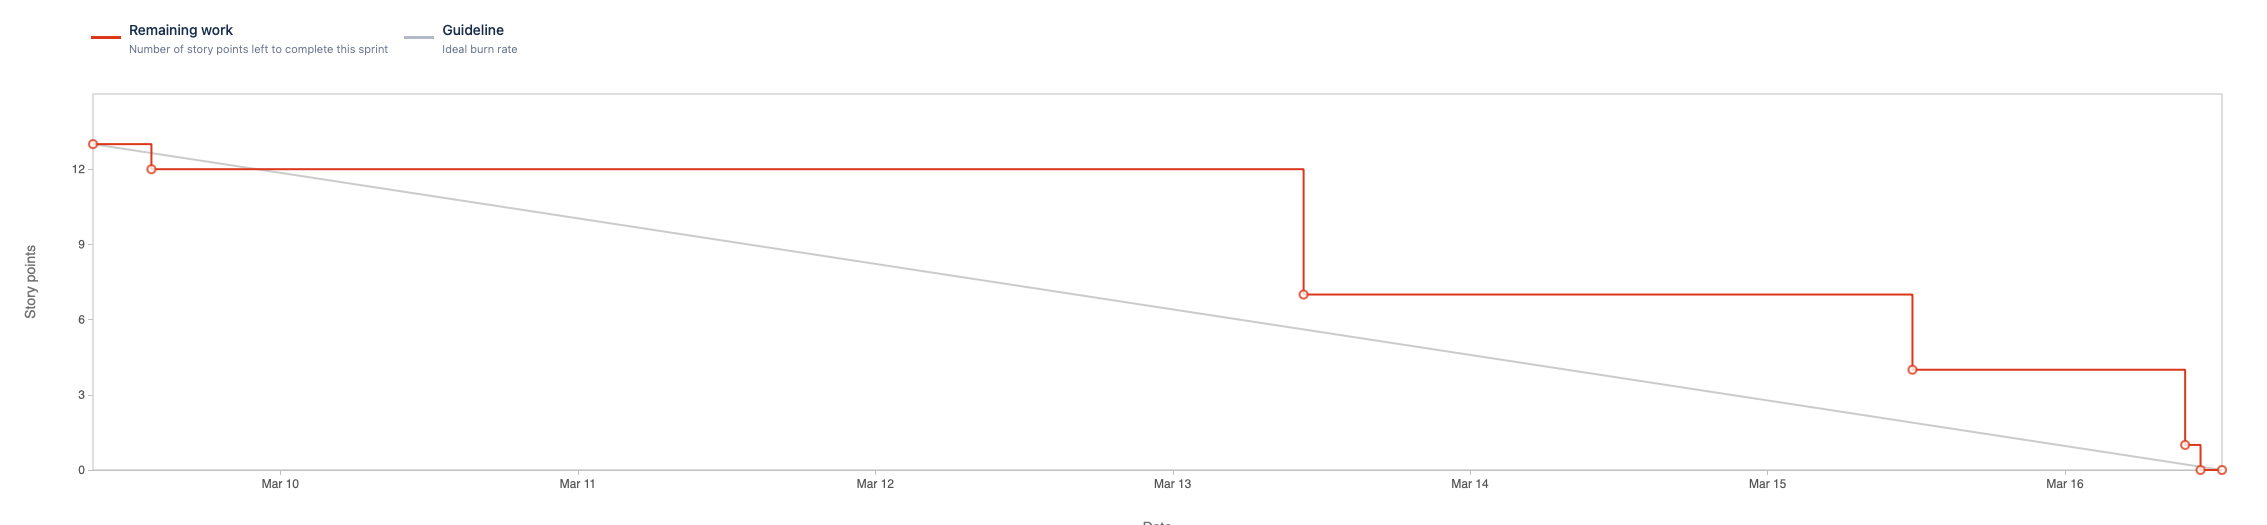
\includegraphics[width=1.0\textwidth]{img/sprint/sprint6.png}
    \caption{Sprint 6} \label{Img:Sprint+6}
\end{figure} 

\subsection{Sprint 7 (09/03/23 - 16/03/23)}\label{sprint-0-090223---160323}
Durante este sprint se comenzó a trabajar en el desarrollo de los endpoints para crear, editar, eliminar y actualizar los datos del usuario. Asimismo, se agregó el requisito de que los usuarios administradores puedan dar de baja un usuario o no permitir algún ingreso debido a actitud sospechosa.\\
Favor apreciar el gráfico de burndown chart referente a ejecución de las tareas en este sprint, (ver figura~\ref{Img:Sprint+7}).

\begin{figure}[h]
    \centering
    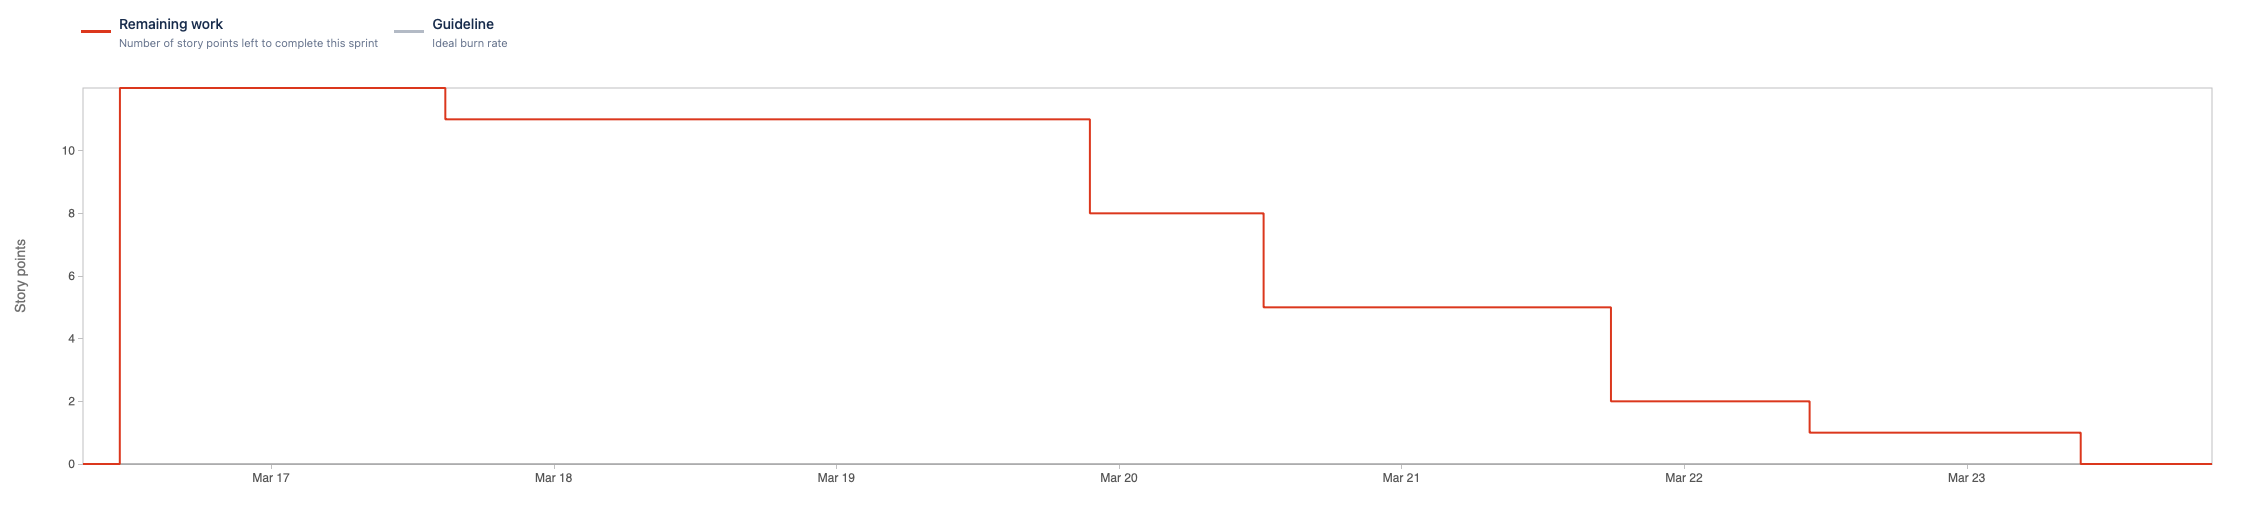
\includegraphics[width=1.0\textwidth]{img/sprint/sprint7.png}
    \caption{Sprint 7} \label{Img:Sprint+7}
\end{figure} 

\subsection{Sprint 8 (23/03/23 - 30/03/23)}\label{sprint-0-230323---300323}
En este sprint se trabajó para agregar la capa de seguridad a los endpoints, mediante el uso de JWT (JSON Web Token), así como también se crearon los test unitarios. El trabajo no fue completado en la fecha pactada debido a inconvenientes en cuanto a conocimiento sobre la validación del token JWT en el middleware de la API.\\
Favor apreciar el gráfico de burndown chart referente a ejecución de las tareas en este sprint, (ver figura~\ref{Img:Sprint+8}).

\begin{figure}[h]
    \centering
    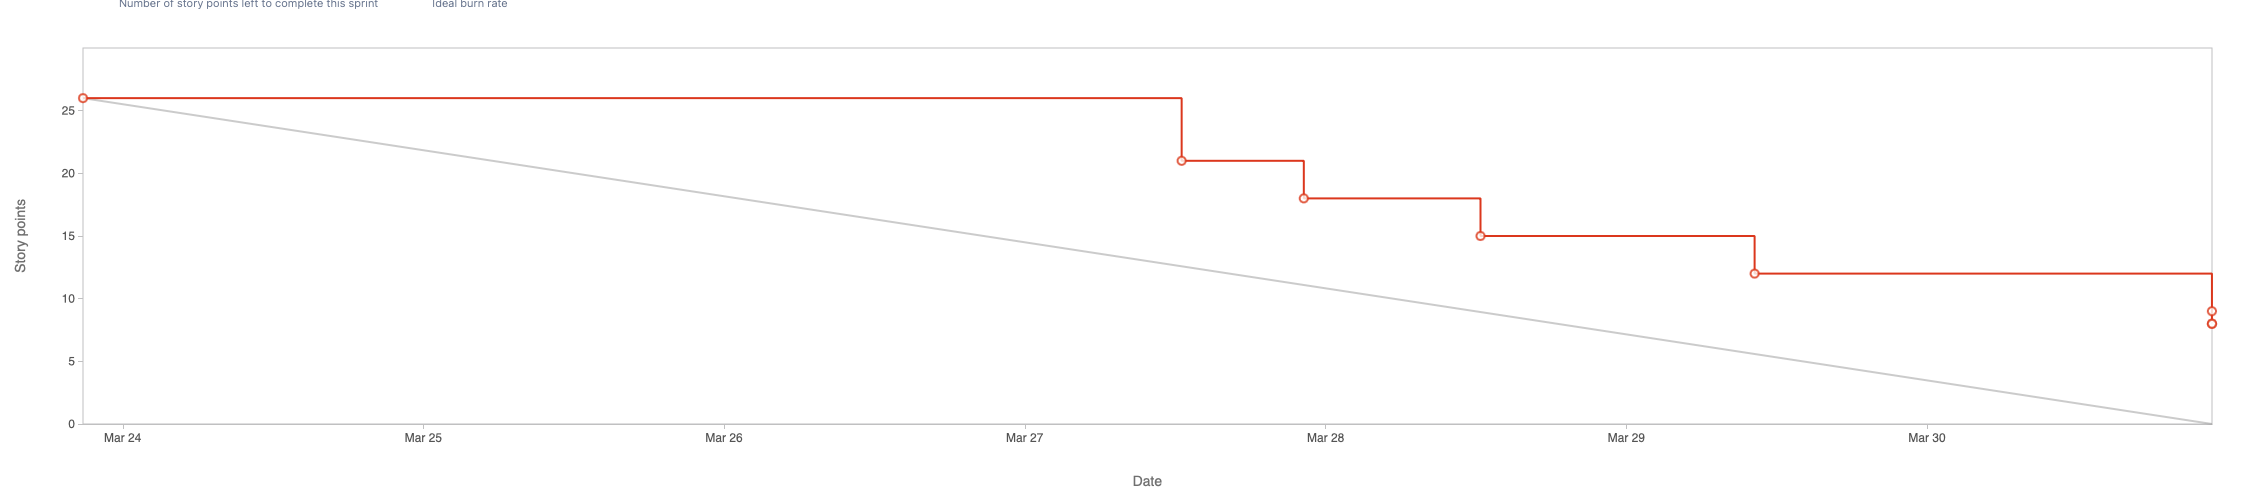
\includegraphics[width=1.0\textwidth]{img/sprint/sprint8.png}
    \caption{Sprint 8} \label{Img:Sprint+8}
\end{figure} 

\subsection{Sprint 9 (31/03/23 - 07/04/23)}\label{sprint-0-310323---070423}
Durante este sprint se pudo desbloquear el trabajo con JWT y se avanzó en la creación de los endpoints para los artículos. Asimismo, se modificó la forma de trabajar respecto a generar tipos de endpoints según características, como por ejemplo para deporte, ocio, recetas, etc, ello se resolvió utilizando el tipo artículos con un filtro por categorías.\\
Favor apreciar el gráfico de burndown chart referente a ejecución de las tareas en este sprint, (ver figura~\ref{Img:Sprint+9}).
\begin{figure}[h]
    \centering
    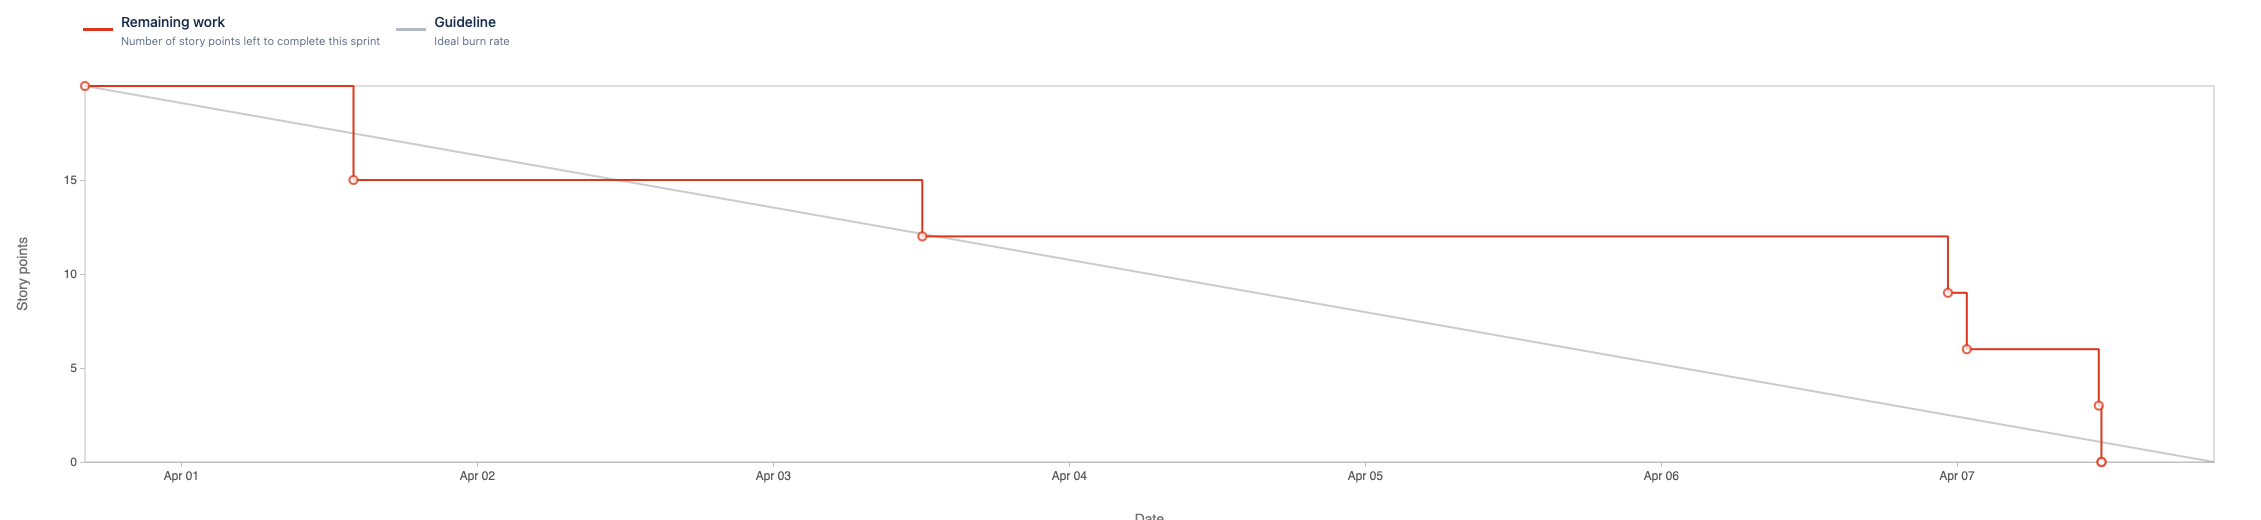
\includegraphics[width=1.0\textwidth]{img/sprint/sprint9.png}
    \caption{Sprint 9} \label{Img:Sprint+9}
\end{figure}

\subsection{Sprint 10 (09/04/23 - 23/04/23)}\label{sprint-0-090423---230422}
En este sprint se trabajó en el desarrollo de preguntas y respuestas, manejo de roles, perfil y actualización de usuario.\\
Favor apreciar el gráfico de burndown chart referente a ejecución de las tareas en este sprint, (ver figura~\ref{Img:Sprint+10}).
\begin{figure}[h]
    \centering
    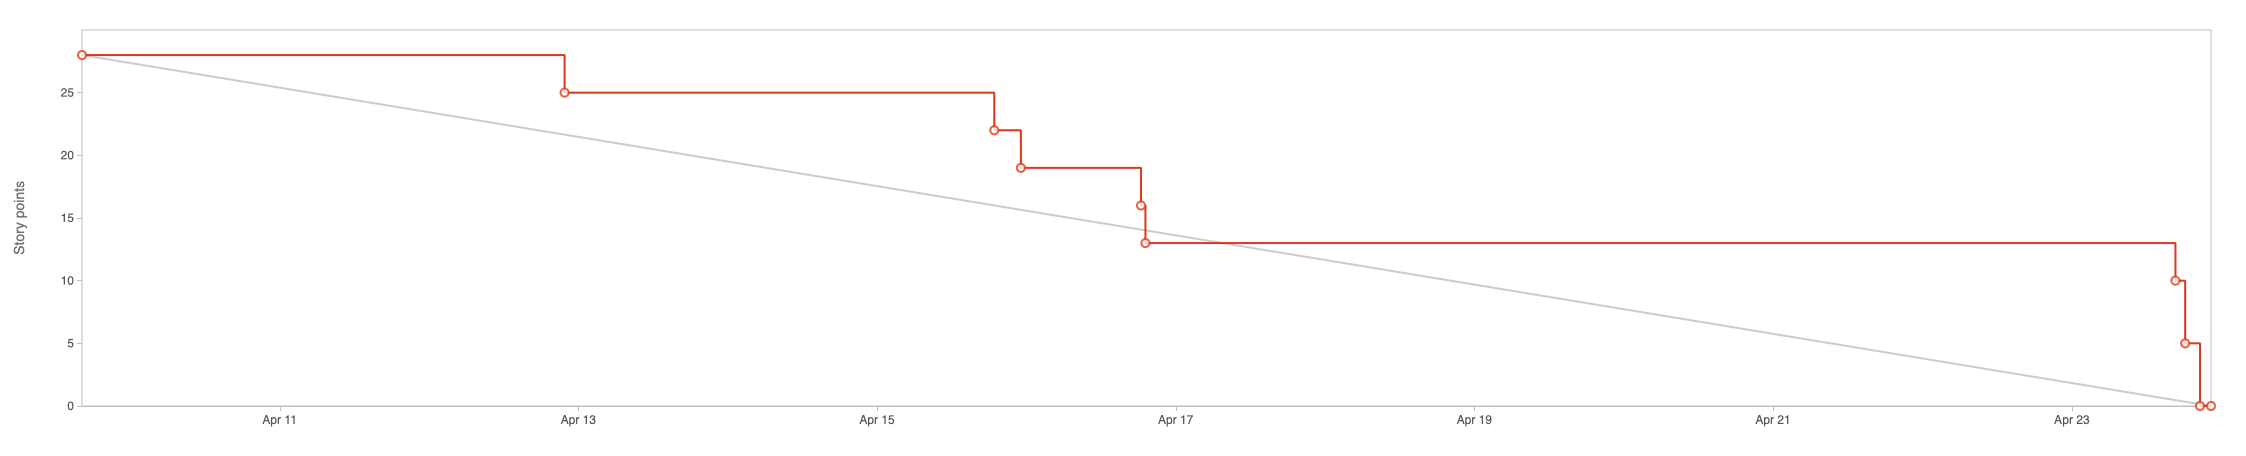
\includegraphics[width=1.0\textwidth]{img/sprint/sprint10.png}
    \caption{Sprint 10} \label{Img:Sprint+10}
\end{figure} 

\subsection{Sprint 11 (25/04/23 - 08/05/23)}\label{sprint-0-250423---080523}
En este sprint se trabajó con la eliminación de recetas y la actualización de las mismas, esto insumió trabajo debido a la eliminación de archivos adjuntos como por ejemplo imágenes.\\
Favor apreciar el gráfico de burndown chart referente a ejecución de las tareas en este sprint, (ver figura~\ref{Img:Sprint+11}).
\begin{figure}[h]
    \centering
    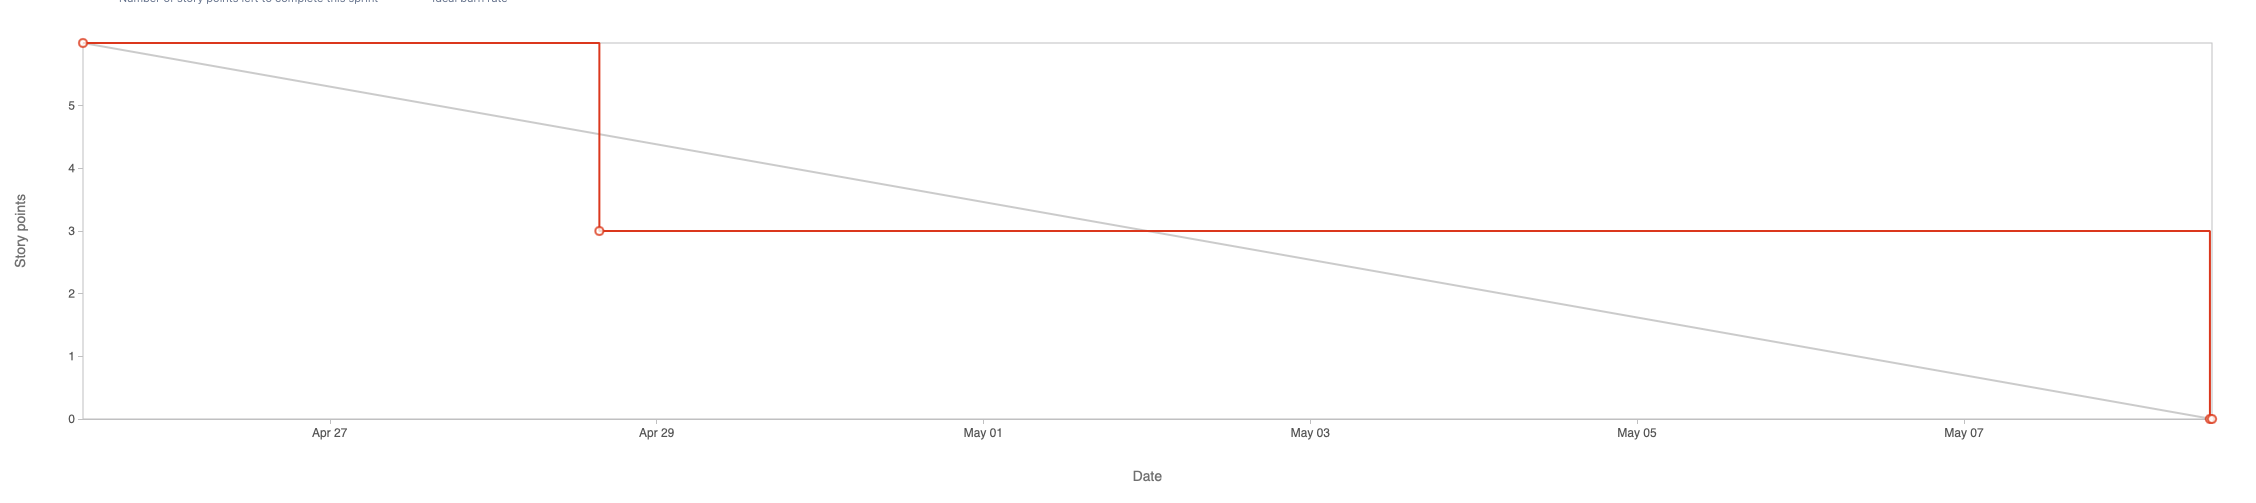
\includegraphics[width=1.0\textwidth]{img/sprint/sprint11.png}
    \caption{Sprint 11} \label{Img:Sprint+11}
\end{figure} 

\subsection{Sprint 12 (08/05/23 - 12/06/23)}\label{sprint-0-250423---080523}
En este sprint el alcance fue mayor, comprendiendo el desarrollo de muchas funcionalidades importantes, como la ficha de seguimiento del paciente, recordatorios, listado de médicos, mapas e interacción con la API externa para procesar datos del clima. \\
Favor apreciar el gráfico de burndown chart referente a ejecución de las tareas en este sprint, (ver figura~\ref{Img:Sprint+12}).
\begin{figure}[h]
    \centering
    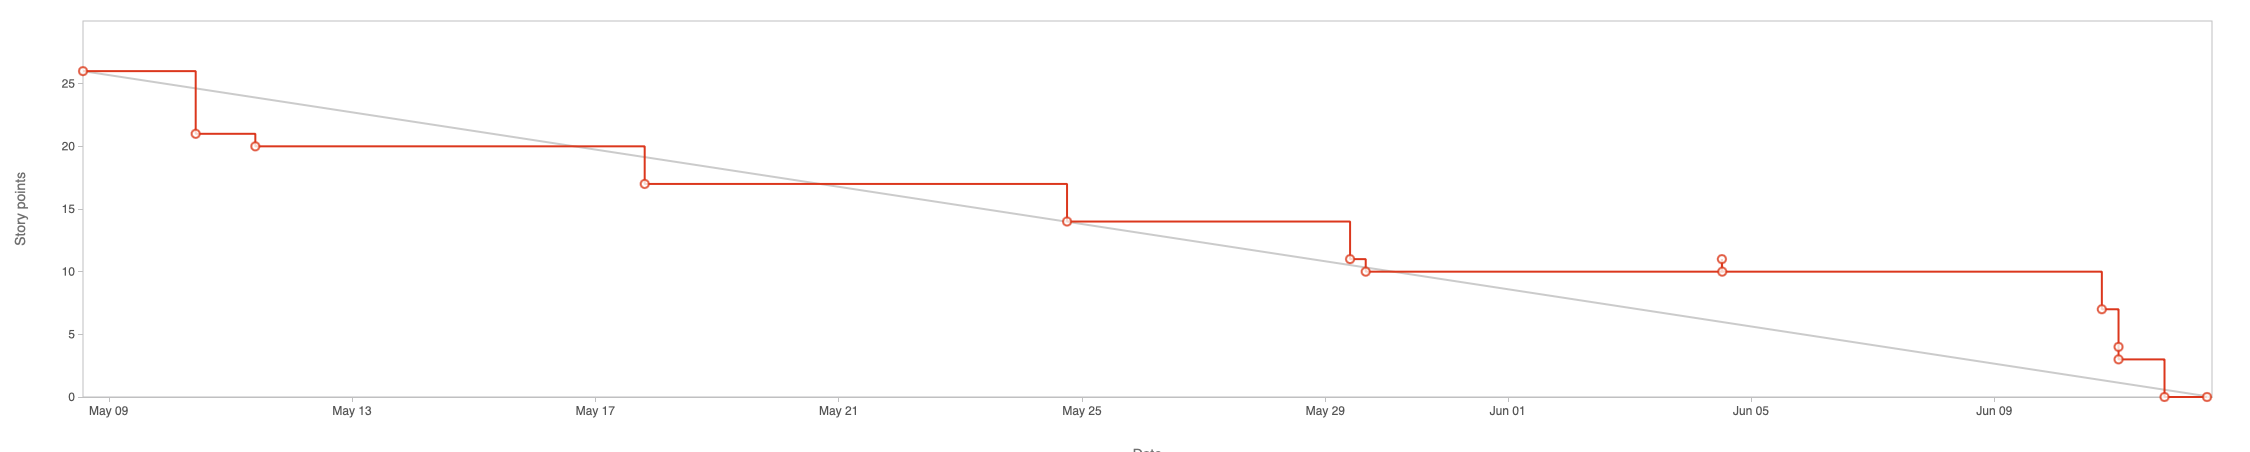
\includegraphics[width=1.0\textwidth]{img/sprint/sprint12.png}
    \caption{Sprint 12} \label{Img:Sprint+12}
\end{figure} 
\newpage
\subsection{Sprint 13 (12/06/23 - 18/06/23)}\label{sprint-0-120623---180623}
Durante este sprint se creó el chatbot que implicó un reto técnico así como en cuanto a conocimiento. Para ello, fue necesario crear el repositorio, el script para extraer información de una herramienta de EMUR (\href{https://brujulaem.uy/sitio/}{Brujula EM}), llevar a cabo la creación del motor de procesamiento, generar los vectores con FAISS para busqueda de cercanías y crear la API para el uso del chatbot.\\
Favor apreciar el gráfico de burndown chart referente a ejecución de las tareas en este sprint, (ver figura~\ref{Img:Sprint+13}).
\begin{figure}[h]
    \centering
    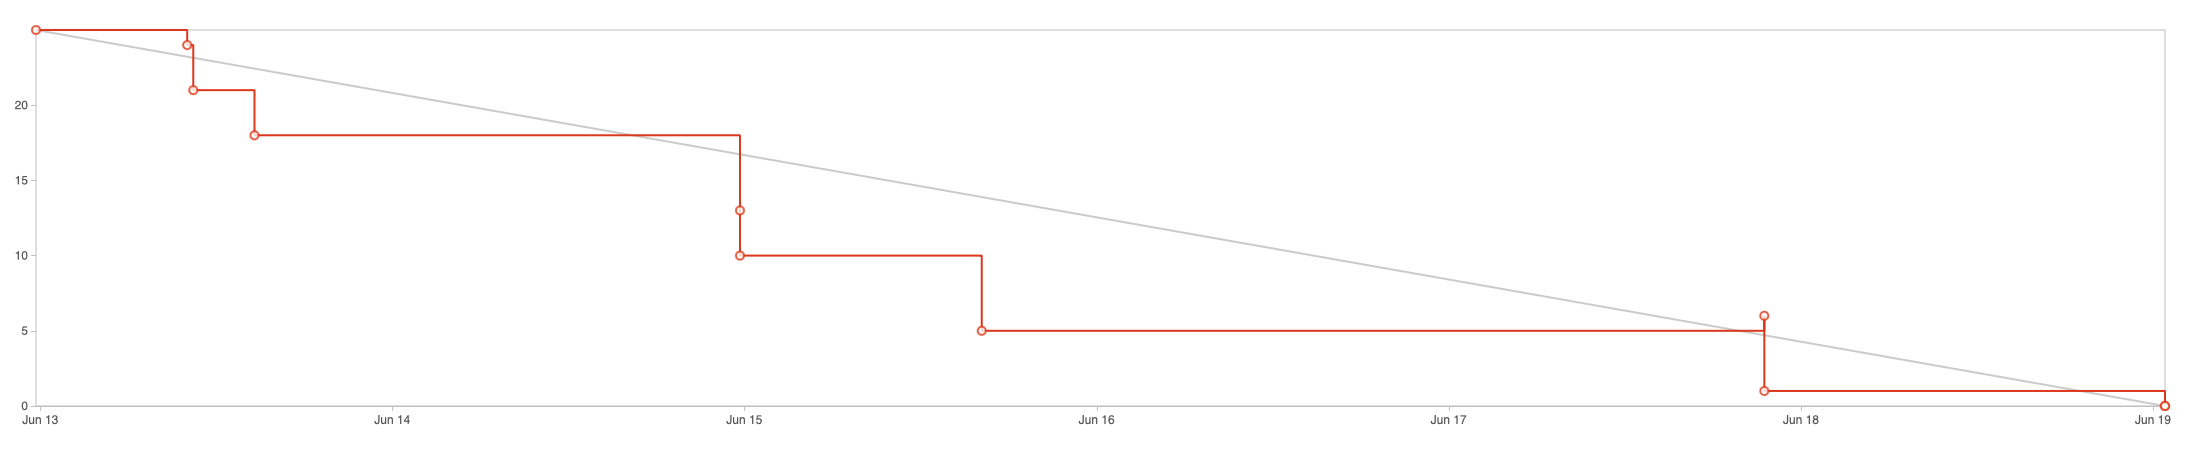
\includegraphics[width=1.0\textwidth]{img/sprint/sprint13.png}
    \caption{Sprint 13} \label{Img:Sprint+13}
\end{figure} 

\subsection{Sprint 14 (22/06/23 - 29/06/23)}\label{sprint-0-220623---290623}
Se generó todo los correspondiente a la documentación de los endpoints utilizando Swagger así como también se hizo el deploy a producción de los microservicios. Es de notar que en este sprint la ejecución fue más rápida debido a conocimientos previamente adquiridos a nivel laboral. \\
Favor apreciar el gráfico de burndown chart referente a ejecución de las tareas en este sprint, (ver figura~\ref{Img:Sprint+14}).
\begin{figure}[h]
    \centering
    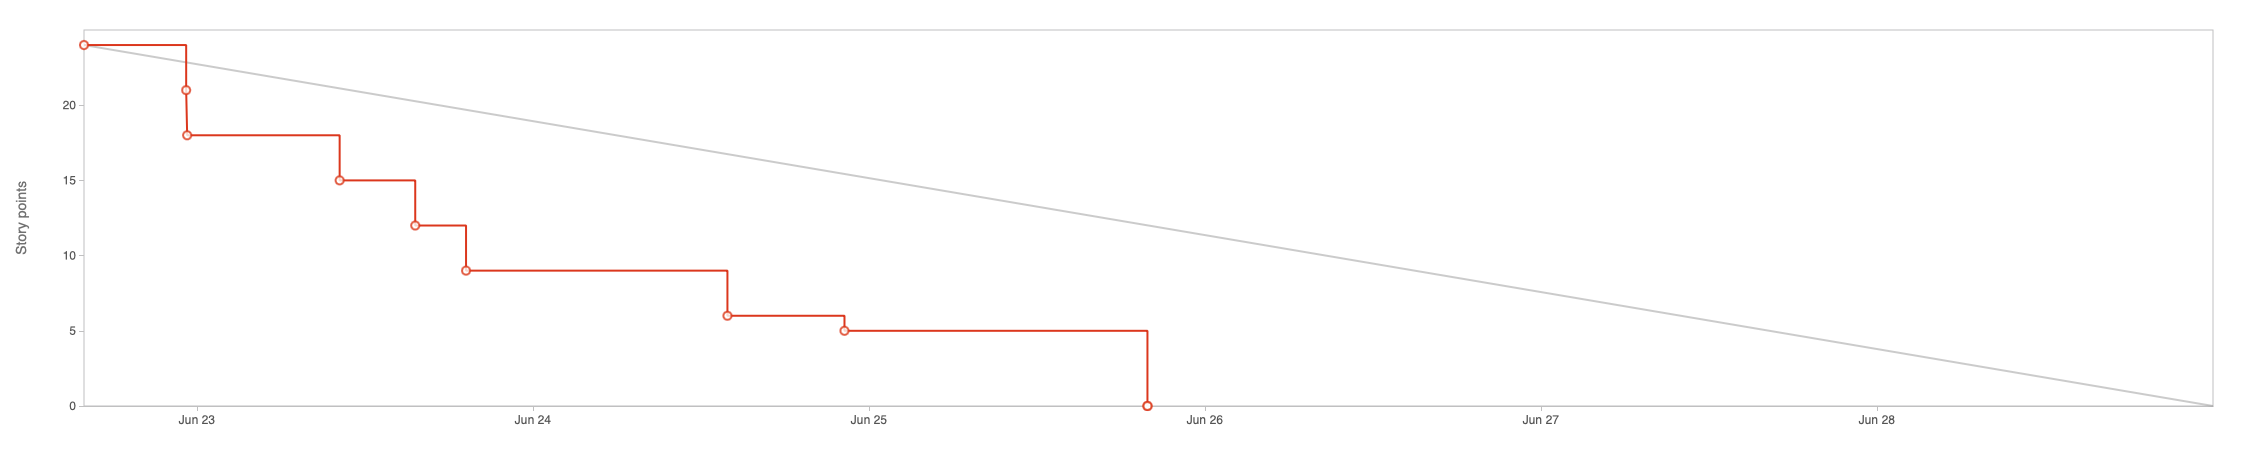
\includegraphics[width=1.0\textwidth]{img/sprint/sprint14.png}
    \caption{Sprint 14} \label{Img:Sprint+14}
\end{figure} 

\section{Estudio de viabilidad}
Un estudio de viabilidad es un análisis exhaustivo, desde diferentes perspectivas, que se realiza para determinar si un proyecto es factible y viable, o no. Este estudio facilita la toma de decisiones y permite identificar las fortalezas, debilidades, oportunidades y amenazas del proyecto.

\subsection{Viabilidad económica}
Un los aspectos clave dentro del estudio de viabilidad, es el económico, puesto que abarca el análisis de los costos en lo que se incurriría de implementarse el proyecto, en contraste con los posibles beneficios que se obtendrán tras su culminación. Así, a continuación, se muestran y analizan los costos y beneficios aproximados derivados del presente proyecto.

\subsubsection{Costes}
La estructura de costes del presente proyecto puede desglosarse en cuatro partidas: costes de personal, costes de hardware, costes de software y costes varios.
\subsubsection{Costes de personal:}
En este caso, el proyecto fue desarrollado por un único participante, en un período aproximado de 600 horas, durante 5 meses, a razón de 4 horas diarias, es decir, media jornada laboral, lo que equivaldría a 2 meses y medio, a razón de 8 horas diarias (jornada completa), que se redondearían a 3 meses de trabajo. Se ha estimado un salario neto de 715,55 USD en base a lo que suele cobrar un desarrollador en Uruguay. Esto se refleja en la tabla~\ref{tab:CostePersonal}.

\begin{longtable}[c]{@{}lr@{}}
\toprule
\multicolumn{1}{c}{\textbf{Concepto}} & \multicolumn{1}{c}{\textbf{Coste}} \\* \midrule
\endfirsthead
%
\endhead
%
\bottomrule
\endfoot
%
\endlastfoot
%
Salario mensual bruto & 890 USD \\
Seguridad Social & 174.45 USD (19,60\%) \\
Salario mensual neto & 715.55 USD \\
\hline
\textbf{Total 3 meses} & \textbf{2.146,65 USD} \\* \bottomrule \\
\caption{Coste mensual del personal}
\label{tab:CostePersonal}
\end{longtable}


Los datos necesarios para realizar estos cálculos fueron extraídos del simulador del Banco de Previsión Social \cite{web:bps}, en donde se debe especificar el salario mensual bruto del profesional, para que luego la plataforma haga las deducciones correspondientes al seguro social.

\subsubsection{Costes de hardware:}
Por ser un proyecto de desarrollo de software, el hardware se limitó al uso de una computadora personal amortizada a 5 años. Ver tabla~\ref{tab:CostesHardware}.

\begin{longtable}[c]{@{}lrr@{}}
\toprule
\multicolumn{1}{c}{\textbf{Concepto}} & \multicolumn{1}{c}{\textbf{Coste}} & \multicolumn{1}{c}{\textbf{Coste amortizado}} \\* \midrule
\endfirsthead
%
\endhead
%
\bottomrule
\endfoot
%
\endlastfoot
%
Ordenador portátil & 1.500 USD & 25 USD \\
Total & & 25 USD \\
Total 3 meses & & 75 USD \\ \hline
\caption{Costes de hardware}
\label{tab:CostesHardware}
\end{longtable}

\subsubsection{Costes de software:}

En este apartado se muestran los costos referentes al pago de licencias de software para el desarrollo del backend. Es importante considerar que, a fin de minimizar los costes, se trabajó en su mayoría con softwares gratuitos. Asimismo, al trabajar con un computador MAC no fue necesario pagar la licencia de uso del sistema operativo, como sí ocurre con Windows. Ver tabla~\ref{tab:CostesSoftware}.
\newpage
\begin{longtable}[c]{@{}lr@{}}
\toprule
\multicolumn{1}{c}{\textbf{Concepto}} & \multicolumn{1}{c}{\textbf{Coste Mensual}} \\* \midrule
\endfirsthead
%
\endhead
%
\bottomrule
\endfoot
%
\endlastfoot
%
SonarCloud & 10 USD \\
Digital Ocean & 24 USD \\
Base de datos Digital Ocean & 15 USD \\
Total & 49 USD \\
Total 3 meses & 147 USD \\ \hline
\caption{Costes de Software}
\label{tab:CostesSoftware}
\end{longtable}

\subsubsection{Costes varios:}
Por su parte, en este sección se detallan los costes del proyecto que no refieren ni al personal, ni al hardware o software, pero que aún así fueron necesarios para el desarrollo del backend en cuestión. Ver tabla~\ref{tab:CostesVarios}.

\begin{longtable}[c]{@{}lr@{}}
\toprule
\multicolumn{1}{c}{\textbf{Concepto}} & \multicolumn{1}{c}{\textbf{Coste}} \\* \midrule
\endfirsthead
%
\endhead
%
\bottomrule
\endfoot
%
\endlastfoot
%
Internet (3 meses) & 208,26 USD \\
Servicio eléctrico (3 meses) & 295,80 USD \\
Total & 504,06 USD \\ \hline
\caption{Costes varios}
\label{tab:CostesVarios}
\end{longtable}

\subsubsection{Coste Total:}
Por último, sólo resta sumar los resultados de las partidas anteriores para obtener el coste total del proyecto, lo cual arroja la cifra de 2.725,71 USD. El desglose de esta operación puede verse en la siguiente tabla. Ver tabla~\ref{tab:CostesTotal}

\begin{longtable}[c]{@{}lr@{}}
\toprule
\multicolumn{1}{c}{\textbf{Concepto}} & \multicolumn{1}{c}{\textbf{Coste}} \\* \midrule
\endfirsthead
%
\endhead
%
\bottomrule
\endfoot
%
\endlastfoot
%
Personal & 2.146,65 USD \\
Hardware & 75,00 USD \\
Software & 147 USD \\
Varios & 504,06 USD \\
Total & 2.872,71 USD \\ \hline
\caption{Costes totales}
\label{tab:CostesTotal}
\end{longtable}
\newpage
\subsection{Beneficios}
En vista de que el backend se desarrolló para una fundación sin ánimos de lucro enfocada en ayudar a personas afectadas con la EM, no se preve que la futura aplicación vaya a monetizarse de alguna forma para obtener algún beneficio económico siendo entonces de uso libre y gratuito.

\subsection{Viabilidad legal}
A continuación, se presentan las licencias requeridas para el desarrollo del presente proyecto, tanto del propio backend, como de su documentación, imágenes y vídeos. En este sentido, una licencia “es la facultad o permiso atribuido a una persona para ejercer una actividad, o gozar de ciertas libertades o concesiones fuera de las ordinarias, por situaciones particulares”.\cite{art:licencias}

Existe compatibilidad parcial entre las licencias de software de código abierto, siendo ésta mayor en unos casos que en otros. A continuación, se detallan las licencias de los módulos de terceros utilizados a lo largo de todo el desarrollo:

\begin{itemize}
\tightlist
\item
\textbf{Licencia MIT:} Licencia de software libre con gran flexibilidad que permite utilizar, modificar y distribuir software, al igual que la Apache 2.0 y la BSD-3. La licencia MIT es una de las más permisivas que hay, lo que implica que acepta un amplio uso del software, no tiene restricciones para uso comercial o privado, y no ofrece protección contra el uso de patentes.\\

\item
\textbf{Licencia Apache 2.0:} En comparación con la MIT, esta añade protección expresa contra las patentes, con su cláusula patentabilidad, permitiendo el uso comercial y privado.\\
\item
\textbf{Licencia BSD-3:} Por su parte, la BSD-3 posee políticas similares a la licencia MIT, permite el uso comercial y privado y no posee restricciones para uso comercial y privado. No obstante, viene con un cláusula de responsabilidad limitada.\\
\end{itemize}

Luego del análisis de los diferentes tipos de licencias de los módulos utilizados (ver tabla~\ref{tab:backend-modulo} y tabla~\ref{tab:chatbot-modulo}), se llegó a la conclusión de que la licencia más adecuada para este caso es la ofrecida por \emph{Apache 2.0}, a razón de las siguientes características:

\begin{itemize}
\tightlist
\item
Protección contra patentes: Lo que garantiza que cualquier usuario pueda hacer uso del software por la cláusula de concesión de patentes que proporciona derechos sobre cualquier patente del contribuidor, siempre que sea necesaria para el uso del programa.\\
\item
Permisividad: Los usuarios pueden modificar y distribuir el software sin necesidad de cumplir con otros requisitos especiales.\\
\item
Exención de responsabilidad y garantía: Lo que libera a los desarrolladores de responsabilidades legales si llegasen a producirse fallos de software.\\
\item 
Compatibilidad con otras licencias: Los usuarios podrán combinar el software con programas que estén bajo otras licencias.\\
\item 
 Notificación de cambios: Asegura que los usuarios sean informados de todo cambio o alteración en el código fuente.\\
 \item 
 Proyectos corporativos: Es ideal para este tipo de desarrollos por su flexibilidad y facilidad para inclusión en proyectos comerciales.\\
\end{itemize}

\begin{table}[H]
\centering
\begin{tabular}{llll}
\toprule
Módulo                     & Versión       & Descripción        & Licencia                    \\
\midrule
\texttt{Health Check}       & master & Middleware chequeo de status & MIT               \\
\texttt{AWS SDK }       & v1.44.237 & SDK para subir archivos & Apache 2.0               \\
\texttt{Imaging }       & v1.6.2 & Procesamiento de imágenes & MIT               \\
\texttt{GIN }       & v1.9.0 & Framework GO para APIs & MIT               \\
\texttt{JWT }       & v3.2.2 & Módulo para autenticación & MIT               \\
\texttt{Google UUID}       & v1.3.0 & Generación de UUID:  & BSD-3              \\
\texttt{Viper }       & v1.15.0 & Variables de entorno & MIT   \\     
\texttt{Testify}       & v1.8.2 & Librería para testing unitario & MIT   \\    
\texttt{Crypto}       & v0.10.0 & Biblioteca para criptografía   & BSD-3  \\    
\texttt{Text}       & v0.10.0 & Procesamiento de texto  & BSD-3  \\    
\texttt{Postgres}       & v1.5.0 & Librería para base de datos  & MIT  \\  
\texttt{Gorm}       & v1.24.7 & ORM para Golang  & MIT  \\  
\bottomrule
\end{tabular}
\caption{Licencias de módulos utilizados en el backend}
\label{tab:backend-modulo}
\end{table}


\begin{table}[H]
\centering
\begin{tabular}{llll}
\toprule
Módulo                     & Versión       & Descripción        & Licencia                    \\
\midrule
\texttt{Bs4}       & 4.12.2 & Librería para scrapping & MIT               \\
\texttt{Request}       & v2.31.0 & Librería para solicitudes HTTP & Apache 2.0               \\
\texttt{Urllib3}       & v2.0.3 & Cliente HTTP para Python & MIT               \\
\texttt{Alembic}       & v1.11.1 & Librería para migraciones & MIT               \\
\texttt{Dotenv}       & v1.0.0 & Variables de entorno & BSD-3               \\
\texttt{Psycopg2}       & v2.9.6 & Librería para base de datos & LGPL               \\
\texttt{Flask}       & v2.3.2 & Framework Python para APIs & BSD-3               \\
\texttt{Flasgger}       & v0.9.7b2 & Documentación Swagger & MIT               \\
\texttt{Gunicorn}       & v20.1.0 & Servidor Python & MIT               \\
\texttt{Langchain}       & v0.0.210 & Construcción de LLM & BSD-3               \\
\texttt{Gevent}       & v22.10.2 & Librería para corutinas & BSD-3               \\
\texttt{OpenAI}       & v0.27.8 & Librería para API OPENAI & BSD-3               \\
\texttt{Faiss}       & v1.7.4 & Similitud y agrupamiento de vectores & BSD-3               \\
\bottomrule
\end{tabular}
\caption{Licencias de módulos utilizados en el chatbot}
\label{tab:chatbot-modulo}
\end{table}
\apendice{Especificación de Requisitos}

\section{Introducción}
A continuación, se detallan los requisitos con los que cumplen la APIs desarrolladas que servirán de base también para la futura implementación de la aplicación móvil.
A este respecto, se siguieron las recomendaciones y lineamientos establecidos por norma IEEE 830-1998, que indica las características que debe tener un documento de especificación de requisitos de software \cite{ieee_830_1998_recommended}; a saber:

\begin{itemize}
\tightlist
\item
  \textbf{Corrección}: Todo requisito contenido en el documento, e implementado en el sistema, es válido si responde a un necesidad real, conduciendo al desarrollo de un sistema deseado.\\
\item
  \textbf{No ambiguo}: Cada requisito debe ser detallado de forma explícita y no prestarse a múltiples interpretaciones. \\
\item
  \textbf{Completo}: Todos los requisitos relevantes están contenidos en el documento de especificación de requisitos del sistema. \\
\item
  \textbf{Consistente}: No puede existir contradicción entre los requisitos del sistema, porque dicha situación imposibilitaría su implementación. \\
\item
  \textbf{Clasificado}: No todos los requisitos tienen el mismo nivel de relevancia para el sistema, por lo que éstos deben clasificarse bien sea según su importancia o por su estabilidad, lo cual permitirá enfocar los recursos en donde realmente se necesitan. \\
\item
  \textbf{Verificable}: El documento es verificable si sus requisitos se pueden poner a prueba de forma experimental a través de un proceso definido y no costoso que ayude a validar su funcionamiento. \\
\item
  \textbf{Modificable}: El documento debe estar estructurado de tal forma que puedan efectuarse cambios en los requisitos de manera fácil, completa y consistente. \\
\item
  \textbf{Trazable}: Se debe conocer el origen de cada requisito al mismo tiempo que se referencia cada uno a los componentes de diseño e implementación. \\
\end{itemize}

\section{Objetivos generales}

El presente proyecto persigue los siguientes objetivos generales en cuanto a las características que debe cumplir el backend: 

\begin{itemize}
    \item Ser eficiente y eficaz para el procesamiento y manipulación de datos.
    \item Presentar una sólida, coherente y confiable lógica de negocio. 
    \item Ponderar la seguridad, privacidad e integridad de la información sensible que los usuarios comparten.
    \item Permitir una robusta escalabilidad y rendimiento del sistema.
    \item Permitir que el sistema se integre con servicios internos y externos tales como APIs.
    \item Habilitar un monitoreo y un registro de errores que haga al sistema tolerante a fallos. 
\end{itemize}

\section{Catálogo de requisitos}

\begin{itemize}
\tightlist
\item
  \textbf{RF-1 Gestión de usuarios:} La API debe permitir el manejo de usuarios.\\
  \begin{itemize}
  \tightlist
  \item
    \textbf{RF-1.1 Registro de usuario:} Permite al usuario registrarse en el sistema.\\
  \item
    \textbf{RF-1.2 Autenticación del usuario:} Permite al usuario ingresar al sistema.\\
  \item
    \textbf{RF-1.3 Actualización del usuario:} Permite al usuario actualizar sus datos en el sistema.\\
  \item
    \textbf{RF-1.4 Obtener información del usuario:} Permite al usuario ver todos sus datos registrados.\\
  \item
    \textbf{RF-1.5 Actualizar estado de activación del usuario:} Permite a un administrador desactivar un usuario.\\
  \item
    \textbf{RF-1.6 Actualizar estado de baneo del usuario:} Permite negar el acceso a un usuario debido a conducta sospechosa.\\
\end{itemize}    
\end{itemize}

\begin{itemize}
\tightlist
\item
  \textbf{RF-2 Gestión de artículos:} La API debe permitir el manejo de artículos.\\
  \begin{itemize}
  \tightlist
  \item
    \textbf{RF-2.1 Crear artículo:} Permite al usuario administrador crear artículos. \\
    \begin{itemize}
    \tightlist
    \item
      \textbf{RF-2.2.1: Agregar categoría a un artículo:} El usuario administrador debe poder agregar una categoría al artículo.\\
    \item
      \textbf{RF-2.2.2: Eliminar categoría a un artículo:} El usuario administrador debe poder eliminar una categoría al artículo. \\
    \end{itemize}
  \item
    \textbf{RF-2.2 Obtener artículos:} Permite a todos los usuarios obtener un listado de todos los artículos.\\
  \item
    \textbf{RF-2.3 Actualización de un artículo:} Permite al usuario administrador actualizar un artículo.\\
  \item
    \textbf{RF-2.4 Eliminar un artículo:} Permite al usuario administrador eliminar un artículo\\
\end{itemize}    
\end{itemize}

\begin{itemize}
\tightlist
\item
  \textbf{RF-3 Gestión de categorías:} La API debe permitir gestionar categorías para poder categorizar los contenidos.\\
  \begin{itemize}
  \tightlist
  \item
    \textbf{RF-3.1 Crear categoría:} Permite al usuario administrador crear categorías. \\
  \item
    \textbf{RF-3.2 Obtener categorías:} Permite a todos los usuarios obtener un listado de todos los artículos.\\
  \item
    \textbf{RF-3.3 Actualizar categorías:} Permite al usuario administrador actualizar una categoría.\\
  \item
    \textbf{RF-3.4 Eliminar categorías:} Permite al usuario administrador eliminar un categoría. \\
\end{itemize}    
\end{itemize}

\begin{itemize}
\tightlist
\item
  \textbf{RF-4 Gestión de Preguntas y Respuestas:} La API debe a permitir a los usuarios realizar preguntas y responder dudas sobre la EM.\\
  \begin{itemize}
  \tightlist
  \item
    \textbf{RF-4.1 Crear preguntas:} Permite al usuario crear preguntas. \\
  \item
    \textbf{RF-4.2 Obtener preguntas:} Permite a todos los usuarios obtener un listado de todas las preguntas.\\
      \item
    \textbf{RF-4.3 Responder a preguntas:} Permite a todos los usuarios responder a preguntas.\\
          \item
    \textbf{RF-4.4 Obtener preguntas a respuestas:} Permite a todos los usuarios obtener todas las preguntas y sus respuestas asociadas.\\
    \end{itemize}    
\end{itemize}

\begin{itemize}
\tightlist
\item
  \textbf{RF-5 Gestión recetas:} La API debe permitir a los usuarios administradores crear recetas.\\
  \begin{itemize}
  \tightlist
  \item
    \textbf{RF-5.1 Crear receta:} Permite a los usuarios administradores crear recetas. \\
  \item
    \textbf{RF-5.2 Obtener recetas:} Permite a todos los usuarios obtener un listado de todas las recetas.\\
      \item
    \textbf{RF-5.3 Actualizar receta:} Permite a los usuarios administradores actualizar una receta.\\
          \item
    \textbf{RF-5.4 Eliminar una recetas:} Permite a los usuarios administradores eliminar una receta.\\
              \item
    \textbf{RF-5.5 Votar una receta:} Permite a los usuarios votar del 1 al 5 una receta.\\
\end{itemize}    
\end{itemize}

\begin{itemize}
\tightlist
\item
  \textbf{RF-6 Gestión de médicos:} La API debe a permitir a los usuarios administradores importar una lista de todos los médicos del país. \\
  \begin{itemize}
  \tightlist
  \item
    \textbf{RF-6.1 Crear médicos:} Permite al usuario administrador importar una lista en CSV de médicos. \\
  \item
    \textbf{RF-6.2 Obtener médicos:} Permite a todos los usuarios obtener un listado de los médicos.\\
\end{itemize}    
\end{itemize}


\begin{itemize}
\tightlist
\item
  \textbf{RF-7 Gestión de servicios de salud:} La API debe a permitir a los usuarios administradores gestionar datos de los servicios de salud del país. \\
  \begin{itemize}
  \tightlist
  \item
    \textbf{RF-7.1 Crear servicio de salud:} Permite a los usuarios administradores crear servicios de salud.\\
  \item
    \textbf{RF-7.2 Obtener servicios de salud:} Permite a todos los usuarios obtener un listado de los servicios de salud.\\
\end{itemize}    
\end{itemize}

\begin{itemize}
\tightlist
\item
  \textbf{RF-8 Gestión de recordatorios:} La API debe a permitir a los usuarios crear recordatorios sobre eventos importantes.\\
  \begin{itemize}
  \tightlist
  \item
    \textbf{RF-8.1 Crear recordatorio:} Permite al usuario crear un recordatorio.\\
  \item
    \textbf{RF-8.2 Obtener recordatorios:} Permite al usuario obtener un listado de sus recordatorios.\\
  \item
    \textbf{RF-8.3 Actualizar recordatorio:} Permite al usuario actualizar su recordatorio.\\
  \item
    \textbf{RF-8.4 Eliminar recordatorio:} Permite al usuario eliminar un recordatorio.\\
  \item
    \textbf{RF-8.5 Votar servicio de salud:} Permite al usuario, luego de finalizado el recordatorio del tipo consulta médica, votar la atención del servicio de salud.\\
  \item
    \textbf{RF-8.6 Votar atención del médico:} Permite al usuario, luego de finalizado el recordatorio del tipo de consulta médica, votar la atención del médico.\\
\end{itemize}    
\end{itemize}

\begin{itemize}
\tightlist
\item
  \textbf{RF-9 Gestión de Tratamiento:} La API debe a permitir a los usuarios gestionar sus tratamientos.\\
  \begin{itemize}
  \tightlist
  \item
    \textbf{RF-9.1 Crear tratamiento:} Permite al usuario crear un tratamiento.\\
 \item
    \textbf{RF-9.2 Obtener tratamiento:} Permite al usuario obtener un listado de sus tratamientos.\\
  \item
    \textbf{RF-9.3 Actualizar tratamiento:} Permite al usuario actualizar su tratamiento.\\
 \item
    \textbf{RF-9.4 Eliminar tratamiento:} Permite al usuario eliminar un tratamiento.\\
\end{itemize}    
\end{itemize}


\begin{itemize}
\tightlist
\item
  \textbf{RF-10 Gestión de síntomas:} La API debe a permitir a los usuarios gestionar sus síntomas.\\
  \begin{itemize}
  \tightlist
  \item
    \textbf{RF-10.1 Crear síntoma:} Permite al usuario administrador crear un tipo de síntoma que los usuarios puedan, más tarde, seleccionar para monitorear.\\
 \item
    \textbf{RF-10.2 Asociar síntoma:} Permite asociar un síntoma a su usuario, para realizar su monitoreo.\\
  \item
    \textbf{RF-10.3 Obtener síntomas:} Permite al usuario obtener un listado de síntomas que puede monitorear.\\
 \item
    \textbf{RF-10.4 Desasociar síntoma:} Permite desasociar un síntoma de su usuario que ya no quiere monitorear.\\
\end{itemize}    
\end{itemize}

\begin{itemize}
\tightlist
\item
  \textbf{RF-11 Gestión de monitoreo:} La API debe a permitir a los usuarios llevar un registro de monitoreo de sus síntomas.\\
  \begin{itemize}
  \tightlist
  \item
    \textbf{RF-11.1 Crear monitoreo:} Permite al usuario  guardar un registro de su síntoma en una escala del 1 al 5 diariamente.\\
 \item
    \textbf{RF-11.2 Obtener monitoreo:} Permite al usuario obtener un listado de todos sus síntomas diarios.\\
\end{itemize}    
\end{itemize}


\begin{itemize}
\tightlist
\item
  \textbf{RF-12 Registro médico:} La API debe a permitir a los usuarios cargar su registro médico (historia clínica).\\
  \begin{itemize}
  \tightlist
  \item
    \textbf{RF-12.1 Crear registro:} Permite al usuario registrar todo lo relevante a su salud.\\
 \item
    \textbf{RF-12.2 Obtener registro:} Permite al usuario obtener su registro médico.\\
 \item
    \textbf{RF-12.3 Actualizar registro:} Permite al usuario actualizar su registro médico.
\end{itemize}    
\end{itemize}

\begin{itemize}
\tightlist
\item
  \textbf{RF-13 Servicios en el mapa:} La API debe a permitir a los usuarios administradores cargar puntos de relevancia para la salud para personas con EM.\\
  \begin{itemize}
  \tightlist
  \item
    \textbf{RF-13.1 Crear servicios:} Permite al usuario administrador crear servicios. \\
  \item
    \textbf{RF-13.2 Obtener servicios:} Permite a los usuarios obtener los servicios.\\
  \item
    \textbf{RF-13.3 Actualizar servicios:} Permite al usuario administrador actualizar un servicio. \\
  \item
    \textbf{RF-13.4 Eliminar servicios:} Permite al usuario administrador eliminar un servicios.\\
\end{itemize}    
\end{itemize}

\begin{itemize}
\tightlist
\item
  \textbf{RF-14 Chatbot:} Se debe crear una API para interactuar con un chatbot
  \begin{itemize}
  \tightlist
  \item
    \textbf{RF-14.1 Chat:} Permite a cualquier usuario chatear con el chatbot. 
\end{itemize}    
\end{itemize}

\subsection{Requisitos no funcionales}\label{requisitos-no-funcionales}

\begin{itemize}
\tightlist
\item
  \textbf{RNF-1 Rendimiento:} El tiempo de respuesta del backend, a las solicitudes y operaciones que realizan los usuarios, debe ser de baja latencia para así poder ofrecer una experiencia fluida con mínimos retrasos o periodos de espera.\\
\item
  \textbf{RNF-2 Escalabilidad:} La aplicación debe ser capaz de admitir la adición de nuevas funcionalidades y características, con bajo acoplamiento, en pro de su atemporalidad, vigencia y actualización, de forma tal que puede representar, en todo momento, una solución adecuada para las personas con EM.\\
\item
  \textbf{RNF-3 Disponibilidad:} El backend debe estar desarrollado de tal forma que esté siempre disponible, a la vez que proporciona tiempos de latencia muy bajos.\\
\item
  \textbf{RNF-4 Seguridad:} El backend debe gestionar todos los datos sensibles, implementando medidas de autenticación y tokens que permitan evitar problemas de seguridad y garanticen la protección de los datos.\\
\item
  \textbf{RNF-5 Mantenibilidad:} La arquitectura de desarrollo del backend debe permitir la ejecución de mantenimiento en cada uno de sus módulos, sin que esto suponga problemas en su funcionamiento.\\
\end{itemize}

\section{Especificación de requisitos}\label{especificacion-de-requisitos-1}
En la presente sección se podrá apreciar el diagrama de casos de uso así como también el analísis de cada uno de los requisitos.

\subsection{Diagrama de casos de uso}
En el siguiente digrama de casos de uso se definen las secuencias de acciones que podrán llevar a cabo tanto el usuario administrador como el usuario común, esto nos permitirá observar a alto nivel los elementos claves para poder entender las interacciones que realizará el sistema (ver figura~\ref{Img:Diseno+Casos+de+Uso}).
Asimismo, se puede ver el digrama en el siguiente enlace de \href{https://drive.google.com/file/d/1eJbkHryF-Qa5LxR3RD6JjWvqmUafC0Qa/view?usp=sharing}{draw.io}.

\begin{figure}[h]
    \centering
    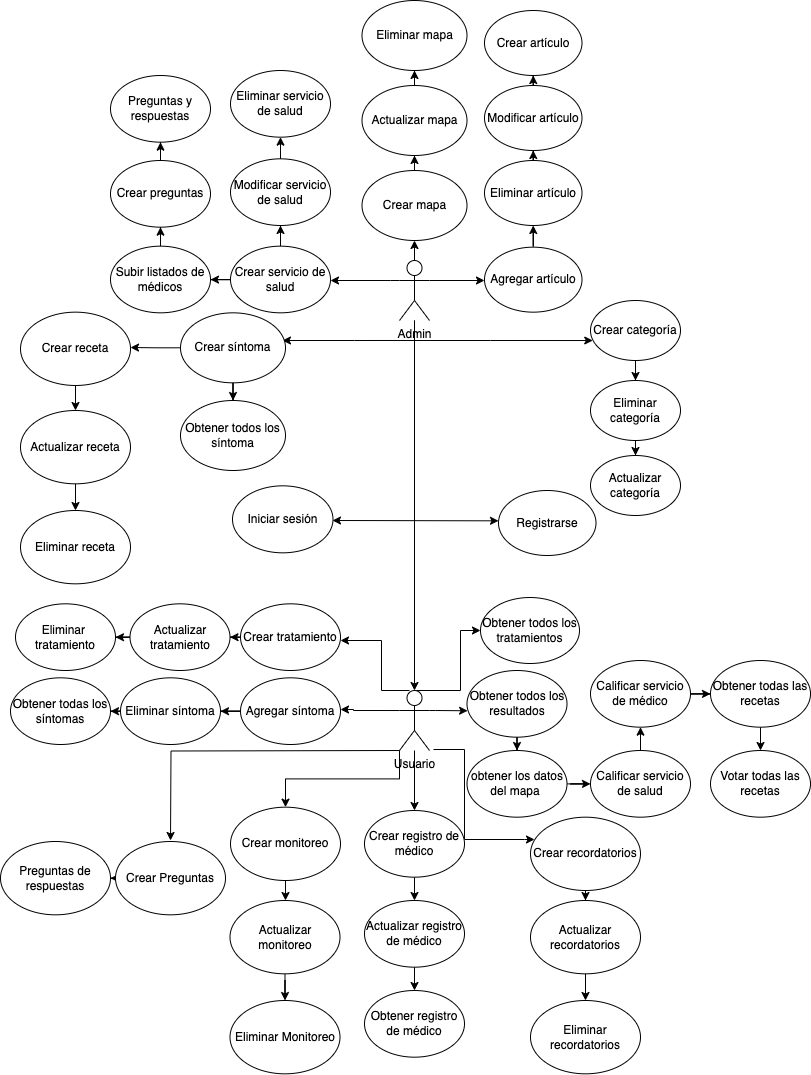
\includegraphics[width=0.7\textwidth]{img/manual/diagrama_casos_de_uso.png}
    \caption{Diagrama de Casos de Uso} \label{Img:Diseno+Casos+de+Uso}
\end{figure} 


% Caso de Uso 1 -> Registro de usuario
\begin{table}[p]
    \centering
    \begin{tabularx}{\linewidth}{ p{0.21\columnwidth} X }
        \toprule
        \textbf{CU-1}    & \textbf{Registro de usuario}\\
        \toprule
        \textbf{Versión}              & 1.0    \\
        \textbf{Autor}                & Roberto Fabián Delgado Pense \\
        \textbf{Requisitos asociados} & RF-1.1 \\ 
        \textbf{Descripción}          & Permite al usuario registrarse en el sistema. \\
        \textbf{Precondición}         & El usuario ha ingresado su dirección de correo electrónico y contraseña. \\
        \textbf{Acciones}             &
        \begin{enumerate}
            \item El sistema verifica las credenciales ingresadas.
            \item Si el correo electrónico y contraseña son válidas, el sistema lo guarda en la base de datos.
            \item El sistema devuelve un mensaje satisfactorio.
        \end{enumerate}\\
        \textbf{Postcondición}        & - \\
        \textbf{Excepciones}          & Si el correo electrónico o la contraseña no cumple los criterios el sistema devuelve un mensaje de error. \\
        \textbf{Importancia}          & Alta \\
        \bottomrule
    \end{tabularx}
    \caption{CU-1 Registro de usuario.}
\end{table}

\begin{table}[p]
    \centering
    \begin{tabularx}{\linewidth}{ p{0.21\columnwidth} X }
        \toprule
        \textbf{CU-2}    & \textbf{Autenticación del usuario}\\
        \toprule
        \textbf{Versión}              & 1.0    \\
        \textbf{Autor}                & Roberto Fabián Delgado Pense \\
        \textbf{Requisitos asociados} & RF-1.2 \\ 
        \textbf{Descripción}          & Permite al usuario ingresar al sistema. \\
        \textbf{Precondición}         & El usuario ha ingresado su dirección de correo electrónico y contraseña. \\
        \textbf{Acciones}             &
        \begin{enumerate}
            \item El sistema verificará las credenciales ingresadas.
            \item Si el correo electrónico y contraseña son válidas, el sistema genera un token JWT válido.
            \item El sistema devuelve el token JWT.
        \end{enumerate}\\
        \textbf{Postcondición}        & El usuario recibe un token JWT válido por 24 horas.\\
        \textbf{Excepciones}          & Si las credenciales ingresadas por el usuario son inválidas, el sistema devuelve una respuesta HTTP con el código 401 (No autorizado) y un mensaje. \\
        \textbf{Importancia}          & Alta \\
        \bottomrule
    \end{tabularx}
    \caption{CU-2 Autenticación del usuario.}
\end{table}

% Caso de Uso 3 -> Actualización de usuario
\begin{table}[p]
	\centering
	\begin{tabularx}{\linewidth}{ p{0.21\columnwidth} p{0.71\columnwidth} }
		\toprule
		\textbf{CU-3}    & \textbf{Actualización del usuario}\\
		\toprule
		\textbf{Versión}              & 1.0    \\
		\textbf{Autor}                & Roberto Fabián Delgado Pense \\
		\textbf{Requisitos asociados} & RF-1.3 \\ 
		\textbf{Descripción}          & Permite al usuario actualizar sus datos. \\
		\textbf{Precondición}         & El usuario se ha autenticado y ha proporcionado información válida para                                             actualizar su perfil. \\
		\textbf{Acciones}             &
		\begin{enumerate}
			\def\labelenumi{\arabic{enumi}.}
			\tightlist
                \item El sistema verifica que el usuario que realiza la solicitud se encuentre autenticado.
			\item El sistema busca al usuario en la base de datos utilizando un identificador único (UUID)                      proporcionado por el token JWT.
                \item El sistema actualiza los datos del usuario en la base de datos.
                \item El sistema devuelve una respuesta de éxito al usuario.
            \end{enumerate}\\
		\textbf{Postcondición}        & Se actualizan los datos del usuario en la base de datos.\\
  		\textbf{Excepciones}          & 
                \begin{enumerate}
			\def\labelenumi{\arabic{enumi}.}
			\tightlist
			\item Si el usuario no se encuentra autenticado el sistema devuelve una respuesta HTTP con el código 401 (No autorizado) y un mensaje.
                \item Si los datos proporcionados por el usuario no son válidos o el usuario no se                           encuentra en la base de datos, el sistema devuelve un mensaje de error. 
            \end{enumerate} \\
		\textbf{Importancia}          & Alta \\
		\bottomrule
	\end{tabularx}
	\caption{CU-3 Actualización del usuario.}
\end{table}

% Caso de Uso 4 -> Obtener información del usuario
\begin{table}[p]
	\centering
	\begin{tabularx}{\linewidth}{ p{0.21\columnwidth} p{0.71\columnwidth} }
		\toprule
		\textbf{CU-4}    & \textbf{Obtener información del usuario}\\
		\toprule
		\textbf{Versión}              & 1.0    \\
		\textbf{Autor}                & Roberto Fabián Delgado Pense \\
		\textbf{Requisitos asociados} & RF-1.4 \\ 
		\textbf{Descripción}          & Permite al usuario obtener su información. \\
		\textbf{Precondición}         & El usuario ha realizado una solicitud para obtener su información personal. \\
		\textbf{Acciones}             &
		\begin{enumerate}
			\def\labelenumi{\arabic{enumi}.}
			\tightlist
			\item El sistema busca al usuario en la base de datos utilizando el identificador único (UUID).
			\item El sistema devuelve la información del usuario que realizó la solicitud.
            \end{enumerate}\\
		\textbf{Postcondición}        & El usuario recibe su propia información personal.\\
		\textbf{Excepciones}          & 
                \begin{enumerate}
			\def\labelenumi{\arabic{enumi}.}
			\tightlist
			\item Si el usuario no se encuentra autenticado el sistema devuelve una respuesta HTTP con el código 401 (No autorizado) y un mensaje.
                \item   Si el usuario no se encuentra en la base de datos, el sistema devuelve un                                            mensaje de error. 
            \end{enumerate}\\
		\textbf{Importancia}          & Alta \\
		\bottomrule
	\end{tabularx}
	\caption{CU-4 Obtener información del usuario.}
\end{table}

% Caso de Uso 5 -> Actualizar el estado de activación del usuario
\begin{table}[p]
	\centering
	\begin{tabularx}{\linewidth}{ p{0.21\columnwidth} p{0.71\columnwidth} }
		\toprule
		\textbf{CU-5}    & \textbf{Actualizar estado de activación del usuario}\\
		\toprule
		\textbf{Versión}              & 1.0    \\
		\textbf{Autor}                & Roberto Fabián Delgado Pense \\
		\textbf{Requisitos asociados} & RF-1.5 \\ 
		\textbf{Descripción}          & Permite al usuario administrador cambiar el estado de un usuario. \\
		\textbf{Precondición}         & Un usuario administrador ha proporcionado un identificador único de usuario y                                              solicita cambiar el estado de activación de un usuario en particular.\\
		\textbf{Acciones}             &
		\begin{enumerate}
			\def\labelenumi{\arabic{enumi}.}
			\tightlist
			\item El sistema busca al usuario en la base de datos utilizando el identificador único (UUID)
                \item El sistema verifica que el usuario que realiza la solicitud se encuentre autenticado y tenga el        permiso de usuario administrador.
			\item El sistema actualiza el estado de activación del usuario en la base de datos, cambiándolo a activo             o inactivo.
                \item El sistema devuelve una respuesta de éxito.
            \end{enumerate}\\
		\textbf{Postcondición}        & Se actualiza el estado de activación del usuario en la base de datos.\\
  
		\textbf{Excepciones}          & 
                \begin{enumerate}
			\def\labelenumi{\arabic{enumi}.}
			\tightlist
			\item Si el usuario no se encuentra autenticado, o no es usuario administrador el sistema devuelve una                 respuesta HTTP con el código 401 (No autorizado) y un mensaje.
                \item   Si el usuario no se encuentra en la base de datos, el sistema devuelve un                                            mensaje de error. 
            \end{enumerate}\\
		\textbf{Importancia}          & Alta \\
		\bottomrule
	\end{tabularx}
	\caption{CU-5 Actualizar estado de activación del usuario.}
\end{table}

% Caso de Uso 6 -> Actualización de estado de baneo de usuario
\begin{table}[p]
	\centering
	\begin{tabularx}{\linewidth}{ p{0.21\columnwidth} p{0.71\columnwidth} }
		\toprule
		\textbf{CU-6}    & \textbf{Actualización del estado de baneo de usuario}\\
		\toprule
		\textbf{Versión}              & 1.0    \\
		\textbf{Autor}                & Roberto Fabián Delgado Pense \\
		\textbf{Requisitos asociados} & RF-1.6 \\ 
		\textbf{Descripción}          & Permite al usuario administrador banear un usuario. \\
		\textbf{Precondición}         & Un usuario administrador ha proporcionado un identificador único de usuario (UUID) y el                                          nuevo estado de baneo para un usuario en particular.\\
		\textbf{Acciones}             &
		\begin{enumerate}
			\def\labelenumi{\arabic{enumi}.}
			\tightlist
                \item El sistema verifica que el usuario que realiza la solicitud se encuentre autenticado y tenga el  permiso de usuario administrador.
			\item El sistema busca al usuario en la base de datos utilizando el identificador único (UUID)
			\item El sistema actualiza el estado de activación del usuario en la base de datos, cambiándolo a activo             o inactivo.
                \item El sistema devuelve una respuesta de éxito.
            \end{enumerate}\\
		\textbf{Postcondición}        & Se actualiza el estado de activación del usuario en la base de datos.\\
		\textbf{Excepciones}          &
              \begin{enumerate}
			\def\labelenumi{\arabic{enumi}.}
			\tightlist
			\item Si el usuario no se encuentra autenticado, o no es usuario administrador, el sistema devuelve una                 respuesta HTTP con el código 401 (No autorizado) y un mensaje.
                \item   Si el usuario no se encuentra en la base de datos, el sistema devuelve un                                            mensaje de error. 
            \end{enumerate}\\
  		\textbf{Importancia}          & Alta \\
		\bottomrule
	\end{tabularx}
	\caption{CU-6 Actualización del estado de baneo de usuario.}
\end{table}

% Caso de Uso 7 -> Crear un artículo
\begin{table}[p]
	\centering
	\begin{tabularx}{\linewidth}{ p{0.21\columnwidth} p{0.71\columnwidth} }
		\toprule
		\textbf{CU-7}    & \textbf{Crear un artículo}\\
		\toprule
		\textbf{Versión}              & 1.0    \\
		\textbf{Autor}                & Roberto Fabián Delgado Pense \\
		\textbf{Requisitos asociados} & RF-2.1, RF-2.2.1, RF-3.2 \\ 
		\textbf{Descripción}          & Permite al usuario administrador crear un artículo. \\
		\textbf{Precondición}         & El usuario administrador ha proporcionado el título, contenido  y imagen para el artículo.\\
		\textbf{Acciones}             &
		\begin{enumerate}
			\def\labelenumi{\arabic{enumi}.}
			\tightlist
			\item El sistema recibe una solicitud HTTP para crear un artículo.
                \item El sistema verifica que el usuario que realiza la solicitud se encuentre autenticado y tenga el permiso de usuario administrador.
			\item El sistema extrae el título, contenido e imagen de la solicitud.
                \item Si la autenticación fue exitosa, el sistema genera un identificador único (UUID) para el artículo.
                \item El sistema guarda el artículo en la base de datos, asociándolo con el identificador del usuario         administrador.
                \item El sistema devuelve una respuesta HTTP con el código 200 (OK) y el artículo creado.            \end{enumerate}\\
		\textbf{Postcondición}        & El artículo fue creado y guardado en la base de datos.\\
		\textbf{Excepciones}          & 
            \begin{enumerate}
			\def\labelenumi{\arabic{enumi}.}
			\tightlist
			\item Si el usuario no se encuentra autenticado, el sistema devuelve una respuesta HTTP con el código            401 (No autorizado).
			\item Si no se proporciona el título, contenido e imagen válida para el artículo, el sistema devuelve una respuesta HTTP con el código 400 (Solicitud incorrecta).
            \end{enumerate}\\
		\textbf{Importancia}          & Alta \\
		\bottomrule
	\end{tabularx}
	\caption{CU-7 Crear un artículo.}
\end{table}

% Caso de Uso 8 -> Obtener todos los artículos
\begin{table}[p]
	\centering
	\begin{tabularx}{\linewidth}{ p{0.21\columnwidth} p{0.71\columnwidth} }
		\toprule
		\textbf{CU-8}    & \textbf{Obtener todos los artículos}\\
		\toprule
		\textbf{Versión}              & 1.0    \\
		\textbf{Autor}                & Roberto Fabián Delgado Pense \\
		\textbf{Requisitos asociados} & RF-2.2 \\ 
		\textbf{Descripción}          & Permite a los usuarios obtener un listado de los                                             artículos. \\
		\textbf{Precondición}         & La base de datos esta disponible. \\
		\textbf{Acciones}             &
		\begin{enumerate}
			\def\labelenumi{\arabic{enumi}.}
			\tightlist
			\item El sistema recibe una solicitud HTTP para obtener todos los artículos.
			\item El sistema verifica que el usuario que realiza la solicitud este autenticado.
                \item Si la autenticación fue exitosa, el sistema recupera todos los artículos guardados en la base        de datos.
                \item El sistema devuelve una respuesta HTTP con el código 200 (OK) y la lista de todos los artículos        recuperados.
            \end{enumerate}\\
		\textbf{Postcondición}        & - \\
		\textbf{Excepciones}          & Si el usuario no se encuentra autenticado, el sistema devuelve una respuesta HTTP con el código            401 (No autorizado) y un mensaje. \\
		\textbf{Importancia}          & Media \\
		\bottomrule
	\end{tabularx}
	\caption{CU-8 Obtener todos los artículos.}
\end{table}

% Caso de Uso 9 -> Actualizar un artículo
\begin{table}[p]
	\centering
	\begin{tabularx}{\linewidth}{ p{0.21\columnwidth} p{0.71\columnwidth} }
		\toprule
		\textbf{CU-9}    & \textbf{Actualizar un artículo}\\
		\toprule
		\textbf{Versión}              & 1.0    \\
		\textbf{Autor}                & Roberto Fabián Delgado Pense \\
		\textbf{Requisitos asociados} & RF-2.3, RF-2.2.1, RF-3.2 \\ 
		\textbf{Descripción}          & Permite al usuario administrador actualizar un artículo. \\
		\textbf{Precondición}         & 
  \begin{enumerate}
			\def\labelenumi{\arabic{enumi}.}
			\tightlist
			\item   El usuario administrador ha proporcionado un identificador único (UUID), de artículo existente.
			\item   El usuario administrador ha proporcionado los datos que necesita actualizar en el artículo, incluyendo el título, contenido e imagen.
            \end{enumerate}\\
		\textbf{Acciones}             &
		\begin{enumerate}
			\def\labelenumi{\arabic{enumi}.}
			\tightlist
			\item El sistema recibe una solicitud HTTP para actualizar un artículo.
                \item El sistema verifica que el usuario que realiza la solicitud se encuentre autenticado y tenga el        permiso de usuario administrador.
			\item El sistema extrae el identificador único (UUID) del artículo desde la URL de la solicitud.
                \item Si la autenticación fue exitosa, el sistema busca en la base de datos el artículo usando el identificador único (UUID).
                \item El sistema actualiza el título, contenido e imagen del artículo con los datos proporcionados.
                \item El sistema devuelve una respuesta HTTP con el código 200 (OK) y el artículo actualizado.
            \end{enumerate}\\
		\textbf{Postcondición}        & El artículo fue actualizado en la base de datos con los nuevos datos                                           proporcionados. \\
		\textbf{Excepciones}          & 
            \begin{enumerate}
			\def\labelenumi{\arabic{enumi}.}
			\tightlist
   			\item Si el usuario no se encuentra autenticado, o no es usuario administrador, el sistema devuelve una                 respuesta HTTP con el código 401 (No autorizado) y un mensaje.
                \item Si no se proporciona un identificador único (UUID) válido de un artículo, el sistema devuelve una respuesta HTTP con el código 400 (Solicitud incorrecta).
                \item Si no se proporcionan datos correctos para el título, contenido e imagen para el artículo, el sistema devuelve una respuesta HTTP con el código 400 (Solicitud incorrecta).
            \end{enumerate}\\
		\textbf{Importancia}          & Alta \\
		\bottomrule
	\end{tabularx}
	\caption{CU-9 Actualizar un artículo.}
\end{table}

% Caso de Uso 10 -> Eliminar un artículo
\begin{table}[p]
	\centering
	\begin{tabularx}{\linewidth}{ p{0.21\columnwidth} p{0.71\columnwidth} }
		\toprule
		\textbf{CU-10}    & \textbf{Eliminar un artículo}\\
		\toprule
		\textbf{Versión}              & 1.0    \\
		\textbf{Autor}                & Roberto Fabián Delgado Pense \\
		\textbf{Requisitos asociados} & RF-2.4 \\ 
		\textbf{Descripción}          & Permite al usuario administrador eliminar un artículo. \\
		\textbf{Precondición}         & El usuario administrador ha proporcionado un identificador único (UUID) de artículo existente.\\
		\textbf{Acciones}             &
		\begin{enumerate}
			\def\labelenumi{\arabic{enumi}.}
			\tightlist
			\item El sistema recibe una solicitud HTTP para eliminar un artículo.
                   \item El sistema verifica que el usuario que realiza la solicitud se encuentre autenticado y tenga el  permiso de usuario administrador.
			\item El sistema extrae el identificador único (UUID) del artículo desde la URL de la solicitud.
                \item Si la autenticación fue exitosa, el sistema busca en la base de datos el artículo usando el identificador único (UUID).
                \item El sistema elimina el artículo de la base de datos.
                \item El sistema devuelve una respuesta HTTP con el código 200 (OK) y un mensaje.
            \end{enumerate}\\
		\textbf{Postcondición}        & El artículo fue eliminado de la base de datos.\\
		\textbf{Excepciones}          & 
            \begin{enumerate}
			\def\labelenumi{\arabic{enumi}.}
			\tightlist
   			\item Si el usuario no se encuentra autenticado, o no es usuario administrador, el sistema devuelve una                 respuesta HTTP con el código 401 (No autorizado) y un mensaje.
                \item Si no se proporciona un identificador único (UUID) válido de un artículo, el sistema devuelve una respuesta HTTP con el código 400 (Solicitud incorrecta).
            \end{enumerate}\\
		\textbf{Importancia}          & Alta \\
		\bottomrule
	\end{tabularx}
	\caption{CU-10 Eliminar un artículo.}
\end{table}

% Caso de Uso 11 -> Agregar categoría a un artículo
\begin{table}[p]
	\centering
	\begin{tabularx}{\linewidth}{ p{0.21\columnwidth} p{0.71\columnwidth} }
		\toprule
		\textbf{CU-11}    & \textbf{Agregar categoría a un artículo}\\
		\toprule
		\textbf{Versión}              & 1.0    \\
		\textbf{Autor}                & Roberto Fabián Delgado Pense \\
		\textbf{Requisitos asociados} & RF-xx, RF-xx \\ 
		\textbf{Descripción}          & Permite al usuario administrador agregar una categoría a un artículo. \\
		\textbf{Precondición}         & 
  		\begin{enumerate}
			\def\labelenumi{\arabic{enumi}.}
			\tightlist
			\item El usuario administrador ha proporcionado un identificador único (UUID) de artículo existente.
			\item El usuario administrador ha proporcionado un identificador único (UUID) de categoría existente.
            \end{enumerate}\\
		\textbf{Acciones}             &
		\begin{enumerate}
			\def\labelenumi{\arabic{enumi}.}
			\tightlist
			\item El sistema recibe una solicitud HTTP para agregar una categoría a un artículo.
                \item El sistema verifica que el usuario administrador que realiza la solicitud se encuentre autenticado y tenga el permiso de administrador.
			\item El sistema extrae los identificadores únicos (UUID) del artículo y la categoría desde la                  solicitud.
                \item Si la autenticación fue exitosa, el sistema busca en la base de datos el artículo y la categoría usando los identificadores únicos (UUID).
                \item El sistema asocia el artículo con la categoría en la base de datos.
                \item El sistema devuelve una respuesta HTTP con el código 200 (OK).
            \end{enumerate}\\
		\textbf{Postcondición}        & El artículo fue asociado a la categoría en la base de datos.\\
		\textbf{Excepciones}          & 
            \begin{enumerate}
			\def\labelenumi{\arabic{enumi}.}
			\tightlist
   			\item Si el usuario no se encuentra autenticado, o no es usuario administrador, el sistema devuelve una                 respuesta HTTP con el código 401 (No autorizado) y un mensaje.
                \item Si no se proporciona un identificador único (UUID) válido de un artículo, el sistema devuelve una respuesta HTTP con el código 400 (Solicitud incorrecta).
            \end{enumerate}\\
		\textbf{Importancia}          & Media \\
		\bottomrule
	\end{tabularx}
	\caption{CU-11 Agregar categoría a un artículo.}
\end{table}

% Caso de Uso 12 -> Eliminar categoría de un artículo
\begin{table}[p]
	\centering
	\begin{tabularx}{\linewidth}{ p{0.21\columnwidth} p{0.71\columnwidth} }
		\toprule
		\textbf{CU-12}    & \textbf{Eliminar categoría a un artículo}\\
		\toprule
		\textbf{Versión}              & 1.0    \\
		\textbf{Autor}                & Roberto Fabián Delgado Pense \\
		\textbf{Requisitos asociados} & RF-2.1, RF-3.1, RF-3.4 \\ 
		\textbf{Descripción}          & Permite al usuario administrador eliminar la categoría de un artículo. \\
		\textbf{Precondición}         & El usuario administrador ha proporcionado un identificador único (UUID) de artículo existente. \\
		\textbf{Acciones}             &
		\begin{enumerate}
			\def\labelenumi{\arabic{enumi}.}
			\tightlist
			\item El sistema recibe una solicitud HTTP para agregar una categoría a un artículo.
                \item El sistema verifica que el usuario que realiza la solicitud se encuentre autenticado y tenga el permiso de usuario administrador.
			\item El sistema extrae los identificadores únicos (UUID) del artículo y la categoría desde la                  solicitud.
                \item Si la autenticación fue exitosa, el sistema busca en la base de datos el artículo y la categoría usando los identificadores únicos (UUID).
                \item El sistema asocia el artículo con la categoría en la base de datos.
                \item El sistema devuelve una respuesta HTTP con el código 200 (OK).
            \end{enumerate}\\
		\textbf{Postcondición}        & El artículo fue disociado de la categoría en la base de datos.\\
		\textbf{Excepciones}          & 
            \begin{enumerate}
			\def\labelenumi{\arabic{enumi}.}
			\tightlist
   			\item Si el usuario no se encuentra autenticado, o no es administrador, el sistema devuelve una                 respuesta HTTP con el código 401 (No autorizado) y un mensaje.
                \item Si no se proporciona un identificador único (UUID) válido de un artículo, el sistema devuelve una respuesta HTTP con el código 400 (Solicitud incorrecta).
            \end{enumerate}\\
		\textbf{Importancia}          & Media \\
		\bottomrule
	\end{tabularx}
	\caption{CU-12 Eliminar categoría a un artículo.}
\end{table}

% Caso de Uso 13 -> Crear categoría
\begin{table}[p]
	\centering
	\begin{tabularx}{\linewidth}{ p{0.21\columnwidth} p{0.71\columnwidth} }
		\toprule
		\textbf{CU-13}    & \textbf{Crear categoría}\\
		\toprule
		\textbf{Versión}              & 1.0    \\
		\textbf{Autor}                & Roberto Fabián Delgado Pense \\
		\textbf{Requisitos asociados} & RF-3.1 \\ 
		\textbf{Descripción}          & Permite al usuario administrador crear una categoría. \\
		\textbf{Precondición}         & El usuario tiene permisos de administrador. \\
		\textbf{Acciones}             &
		\begin{enumerate}
			\def\labelenumi{\arabic{enumi}.}
			\tightlist
			\item El sistema recibe una solicitud HTTP para crear una nueva categoría.
                \item El sistema verifica que el usuario que realiza la solicitud se encuentre autenticado y tenga el permiso de usuario administrador.
			\item El sistema valida la solicitud y verifica que los datos para crear la categoría sean correctos.
                \item El sistema crea la categoría en la base de datos.
                \item El sistema devuelve una respuesta HTTP con el código 200 (OK).
            \end{enumerate}\\
		\textbf{Postcondición}        & La categoría fue creada en la base de datos.\\
		\textbf{Excepciones}          & 
            \begin{enumerate}
			\def\labelenumi{\arabic{enumi}.}
			\tightlist
   			\item Si el usuario no se encuentra autenticado, o no es usuario administrador, el sistema devuelve una                 respuesta HTTP con el código 401 (No autorizado) y un mensaje.
            \end{enumerate}\\
		\textbf{Importancia}          & Alta \\
		\bottomrule
	\end{tabularx}
	\caption{CU-13 Crear categoría.}
\end{table}

% Caso de Uso 14 -> Obtener todas las categorías
\begin{table}[p]
	\centering
	\begin{tabularx}{\linewidth}{ p{0.21\columnwidth} p{0.71\columnwidth} }
		\toprule
		\textbf{CU-14}    & \textbf{Obtener todas las categorías}\\
		\toprule
		\textbf{Versión}              & 1.0    \\
		\textbf{Autor}                & Roberto Fabián Delgado Pense \\
		\textbf{Requisitos asociados} & RF-3.2 \\ 
		\textbf{Descripción}          & Permite al usuario administrador obtener todas las categorías. \\
		\textbf{Precondición}         & El usuario tiene permisos de administrador. \\
		\textbf{Acciones}             &
		\begin{enumerate}
			\def\labelenumi{\arabic{enumi}.}
			\tightlist
			\item El sistema recibe una solicitud HTTP para obtener las categorías.
                \item El sistema verifica que el usuario que realiza la solicitud se encuentre autenticado y tenga el permiso de usuario administrador.
			\item El sistema obtiene todas las categorías guardadas en la base de datos.
                \item El sistema devuelve una respuesta HTTP con el código 200 (OK).
            \end{enumerate}\\
		\textbf{Postcondición}        & La categoría fue creada en la base de datos.\\
		\textbf{Excepciones}          & 
            \begin{enumerate}
			\def\labelenumi{\arabic{enumi}.}
			\tightlist
   			\item Si el usuario no se encuentra autenticado, o no es usuario administrador, el sistema devuelve una                 respuesta HTTP con el código 401 (No autorizado) y un mensaje.
                \item Si ocurre un error al obtener las categorías, el sistema devuelve una respuesta con el código de estado 500 Internal Server Error y un mensaje.
            \end{enumerate}\\
		\textbf{Importancia}          & Media \\
		\bottomrule
	\end{tabularx}
	\caption{CU-14 Obtener todas las categorías.}
\end{table}

% Caso de Uso 15 -> Actualizar una categoría
\begin{table}[p]
	\centering
	\begin{tabularx}{\linewidth}{ p{0.21\columnwidth} p{0.71\columnwidth} }
		\toprule
		\textbf{CU-15}    & \textbf{Actualizar una categoría}\\
		\toprule
		\textbf{Versión}              & 1.0    \\
		\textbf{Autor}                & Roberto Fabián Delgado Pense \\
		\textbf{Requisitos asociados} & RF-3.3 \\ 
		\textbf{Descripción}          & Permite al usuario administrador actualizar una categoría. \\
		\textbf{Precondición}         & El usuario tiene permisos de administrador. \\
		\textbf{Acciones}             &
		\begin{enumerate}
			\def\labelenumi{\arabic{enumi}.}
			\tightlist
                \item El sistema verifica que el usuario que realiza la solicitud se encuentre autenticado y tenga el permiso de usuario administrador.
			\item El usuario ha proporcionado un identificador único (UUID), de categoría existente.
			\item El sistema valida la existencia de la categoría en la base de datos.
                \item El sistema actualiza los datos de la categoría con los nuevos valores proporcionados en la solicitud.
                \item El sistema devuelve una respuesta HTTP con el código 200 (OK).
            \end{enumerate}\\
		\textbf{Postcondición}        & La categoría se actualiza correctamente en la base de datos.\\
		\textbf{Excepciones}          & 
            \begin{enumerate}
			\def\labelenumi{\arabic{enumi}.}
			\tightlist
   			\item Si el usuario no se encuentra autenticado, o no es usuario administrador, el sistema devuelve una                 respuesta HTTP con el código 401 (No autorizado) y un mensaje.
                \item   Si la categoría no se encuentra en la base de datos, el sistema devuelve un                           una respuesta HTTP con el código 404 (No encontrado) y un mensaje. 
                \item Si ocurre un error al actualizar la categoría, el sistema devuelve una respuesta con el código de estado 500 (Error interno del servidor) y un mensaje
            \end{enumerate}\\
		\textbf{Importancia}          & Alta \\
		\bottomrule
	\end{tabularx}
	\caption{CU-15 Actualizar una categoría.}
\end{table}

% Caso de Uso 16 -> Eliminar una categoría
\begin{table}[p]
	\centering
	\begin{tabularx}{\linewidth}{ p{0.21\columnwidth} p{0.71\columnwidth} }
		\toprule
		\textbf{CU-16}    & \textbf{Eliminar una categoría}\\
		\toprule
		\textbf{Versión}              & 1.0    \\
		\textbf{Autor}                & Roberto Fabián Delgado Pense \\
		\textbf{Requisitos asociados} & RF-3.4 \\ 
		\textbf{Descripción}          & Permite al usuario administrador eliminar una categoría. \\
		\textbf{Precondición}         & El usuario ha proporcionado un identificador único (UUID) de categoría existente.\\
		\textbf{Acciones}             &
		\begin{enumerate}
			\def\labelenumi{\arabic{enumi}.}
			\tightlist
			\item El sistema recibe una solicitud HTTP para eliminar una categoría.
                   \item El sistema verifica que el usuario que realizar la solicitud se encuentre autenticado y tenga el permiso de usuario administrador.
			\item El sistema extrae el identificador único (UUID) de la categoría desde la URL de la solicitud.
                \item Si la autenticación fue exitosa, el sistema busca en la base de datos la categoría usando el identificador único (UUID).
                \item El sistema elimina la categoría de la base de datos.
                \item El sistema devuelve una respuesta HTTP con el código 200 (OK) y la categoría fue eliminada.
            \end{enumerate}\\
		\textbf{Postcondición}        & La categoría fue eliminada de la base de datos.\\
		\textbf{Excepciones}          & 
            \begin{enumerate}
			\def\labelenumi{\arabic{enumi}.}
			\tightlist
   			\item Si el usuario no se encuentra autenticado, o no es usuario administrador, el sistema devuelve una                 respuesta HTTP con el código 401 (No autorizado) y un mensaje.
                \item   Si la categoría no se encuentra en la base de datos, el sistema devuelve un                           una respuesta HTTP con el código 404 (No encontrado) y un mensaje. 
                \item Si ocurre un error al eliminar la categoría, el sistema devuelve una respuesta con el código de estado 500 (Error interno del servidor) y un mensaje
            \end{enumerate}\\
		\textbf{Importancia}          & Alta \\
		\bottomrule
	\end{tabularx}
	\caption{CU-16 Eliminar una categoría.}
\end{table}

% Caso de Uso 17 -> Crear pregunta
\begin{table}[p]
	\centering
	\begin{tabularx}{\linewidth}{ p{0.21\columnwidth} p{0.71\columnwidth} }
		\toprule
		\textbf{CU-17}    & \textbf{Crear pregunta}\\
		\toprule
		\textbf{Versión}              & 1.0    \\
		\textbf{Autor}                & Roberto Fabián Delgado Pense \\
		\textbf{Requisitos asociados} & RF-4.1 \\ 
		\textbf{Descripción}          & Permite a los usuarios crear preguntas. \\
		\textbf{Precondición}         & El usuario debe estar autenticado.\\
		\textbf{Acciones}             &
		\begin{enumerate}
			\def\labelenumi{\arabic{enumi}.}
			\tightlist
			\item El sistema recibe una solicitud HTTP para crear una pregunta.
                \item El sistema verifica que el usuario que realiza la solicitud este autenticado.
			\item El sistema valida la solicitud y extrae el texto de la pregunta.
                \item El sistema crea una nueva pregunta en la base de datos, asociándola al usuario actual.
                \item El sistema devuelve una respuesta HTTP con el código 200 (OK) y la pregunta creada.            \end{enumerate}\\
		\textbf{Postcondición}        & La pregunta fue creada y guardada en la base de datos.\\
		\textbf{Excepciones}          & 
            \begin{enumerate}
			\def\labelenumi{\arabic{enumi}.}
			\tightlist
			\item Si el usuario no se encuentra autenticado, el sistema devuelve una respuesta HTTP con el código            401 (No autorizado).
			\item Si la solicitud es inválida o los datos de la pregunta son incorrectos para la pregunta, el sistema devuelve una respuesta HTTP con el código 400 (Solicitud incorrecta) y un mensaje de error.
            \end{enumerate}\\
		\textbf{Importancia}          & Alta \\
		\bottomrule
	\end{tabularx}
	\caption{CU-17 Crear pregunta.}
\end{table}

% Caso de Uso 18 -> Obtener todas las preguntas
\begin{table}[p]
	\centering
	\begin{tabularx}{\linewidth}{ p{0.21\columnwidth} p{0.71\columnwidth} }
		\toprule
		\textbf{CU-18}    & \textbf{Obtener todas las preguntas}\\
		\toprule
		\textbf{Versión}              & 1.0    \\
		\textbf{Autor}                & Roberto Fabián Delgado Pense \\
		\textbf{Requisitos asociados} & RF-4.2 \\ 
		\textbf{Descripción}          & Permite a los usuarios obtener todas las  preguntas. \\
		\textbf{Precondición}         & El usuario debe estar autenticado.\\
		\textbf{Acciones}             &
		\begin{enumerate}
			\def\labelenumi{\arabic{enumi}.}
			\tightlist
			\item El sistema recibe una solicitud HTTP para obtener las preguntas.
                \item El sistema verifica que el usuario que realiza la solicitud se encuentre autenticado.
			\item El sistema obtiene todas las preguntas guardadas en la base de datos.
                \item El sistema devuelve una respuesta HTTP con el código 200 (OK).          
            \end{enumerate}\\
		\textbf{Postcondición}        & - \\
		\textbf{Excepciones}          & Si el usuario no se encuentra autenticado, el sistema devuelve una respuesta HTTP con el código 401 (No autorizado). \\
		\textbf{Importancia}          & Media \\
		\bottomrule
	\end{tabularx}
	\caption{CU-18 Obtener todas las preguntas.}
\end{table}

% Caso de Uso 19 -> Crear respuesta a pregunta
\begin{table}[p]
	\centering
	\begin{tabularx}{\linewidth}{ p{0.21\columnwidth} p{0.71\columnwidth} }
		\toprule
		\textbf{CU-19}    & \textbf{Crear respuesta a pregunta}\\
		\toprule
		\textbf{Versión}              & 1.0    \\
		\textbf{Autor}                & Roberto Fabián Delgado Pense \\
		\textbf{Requisitos asociados} & RF-4.3 \\ 
		\textbf{Descripción}          & Permite a los usuarios crear respuesta a una pregunta.\\
		\textbf{Precondición}         & 
  		\begin{enumerate}
			\def\labelenumi{\arabic{enumi}.}
			\tightlist
                \item El usuario debe estar autenticado.
                \item La pregunta a la que va a responder existe en el sistema.
                \end{enumerate}\\
            \textbf{Acciones}             &
		\begin{enumerate}
			\def\labelenumi{\arabic{enumi}.}
			\tightlist
			\item El sistema recibe una solicitud HTTP para crear una respuesta a una pregunta.
                \item El sistema verifica que el usuario que realiza la solicitud este autenticado.
			\item El sistema extrae el identificador único (UUID) de la pregunta desde la URL de la solicitud.
			\item El sistema valida la solicitud y extrae el texto de la respuesta.
                \item El sistema crea una nueva respuesta a la pregunta en la base de datos, asociándola al usuario actual.
                \item El sistema devuelve una respuesta HTTP con el código 200 (OK) y la respuesta creada.            \end{enumerate}\\
		\textbf{Postcondición}        & La respuesta fue creada y guardada en la base de datos.\\
		\textbf{Excepciones}          & 
            \begin{enumerate}
			\def\labelenumi{\arabic{enumi}.}
			\tightlist
			\item Si el usuario no se encuentra autenticado, el sistema devuelve una respuesta HTTP con el código            401 (No autorizado).
			\item Si la solicitud es inválida o los datos de la respuesta son incorrectos para la pregunta, el sistema devuelve una respuesta HTTP con el código 400 (Solicitud incorrecta) y un mensaje de error.
            \end{enumerate}\\
		\textbf{Importancia}          & Alta \\
		\bottomrule
	\end{tabularx}
	\caption{CU-19 Crear respuesta a pregunta.}
\end{table}

% Caso de Uso 20 -> Obtener todas las respuestas de una pregunta
\begin{table}[p]
	\centering
	\begin{tabularx}{\linewidth}{ p{0.21\columnwidth} p{0.71\columnwidth} }
		\toprule
		\textbf{CU-20}    & \textbf{Obtener todas las respuestas de una pregunta}\\
		\toprule
		\textbf{Versión}              & 1.0    \\
		\textbf{Autor}                & Roberto Fabián Delgado Pense \\
		\textbf{Requisitos asociados} & RF-4.4 \\ 
		\textbf{Descripción}          & Permite a los usuarios obtener todas las  respuestas a una pregunta. \\
		\textbf{Precondición}         & 
  		\begin{enumerate}
			\def\labelenumi{\arabic{enumi}.}
			\tightlist
			\item El usuario debe estar autenticado en el sistema.
                \item La pregunta debe existir en el sistema.        
            \end{enumerate}\\
            
		\textbf{Acciones}             &
		\begin{enumerate}
			\def\labelenumi{\arabic{enumi}.}
			\tightlist
			\item El sistema recibe una solicitud HTTP para obtener todas las respuestas de una pregunta         
                        específica.
                \item El sistema verifica que el usuario que realiza la solicitud se encuentre autenticado.
			\item El sistema obtiene todas las respuestas relacionada a una pregunta guardada en la base de datos.
                \item El sistema devuelve una respuesta HTTP con el código 200 (OK).          
            \end{enumerate}\\
		\textbf{Postcondición}        & - \\
		\textbf{Excepciones}          & 
              \begin{enumerate}
			\def\labelenumi{\arabic{enumi}.}
			\tightlist
			\item   Si el usuario no se encuentra autenticado, el sistema devuelve una respuesta HTTP con el código 401 (No autorizado).
			\item Si no existen respuestas para la pregunta se retorna un array vacío.
            \end{enumerate}\\
		\textbf{Importancia}          & Media \\
		\bottomrule
	\end{tabularx}
	\caption{CU-20 Obtener todas las respuestas de una pregunta.}
\end{table}

% Caso de Uso 21 -> Crear receta
\begin{table}[p]
	\centering
	\begin{tabularx}{\linewidth}{ p{0.21\columnwidth} p{0.71\columnwidth} }
		\toprule
		\textbf{CU-21}    & \textbf{Crear receta}\\
		\toprule
		\textbf{Versión}              & 1.0    \\
		\textbf{Autor}                & Roberto Fabián Delgado Pense \\
		\textbf{Requisitos asociados} & RF-5.1 \\ 
		\textbf{Descripción}          & Permite a los usuarios administradores crear recetas. \\
		\textbf{Precondición}         & El usuario tiene permiso de usuario administrador. \\  
		\textbf{Acciones}             &
		\begin{enumerate}
			\def\labelenumi{\arabic{enumi}.}
			\tightlist
			\item El sistema recibe una solicitud HTTP para crear una receta.
                \item El sistema verifica que el usuario que realiza la solicitud se encuentre autenticado y tenga el permiso de usuario administrador.
                \item El sistema valida la solicitud y extrae el nombre, ingredientes, elaboración, tiempo,     imagenes y categoría.
                \item El sistema crea la receta en la base de datos.
                \item El sistema devuelve una respuesta HTTP con el código 200 (OK) y los datos insertados.         
            \end{enumerate}\\
		\textbf{Postcondición}        & La receta fue creada en la base de datos. \\
		\textbf{Excepciones}          & 
              \begin{enumerate}
			\def\labelenumi{\arabic{enumi}.}
			\tightlist
   			\item Si el usuario no se encuentra autenticado, o no es usuario administrador, el sistema devuelve una                 respuesta HTTP con el código 401 (No autorizado) y un mensaje.
                \item   Si la receta no pudo ser creada en la base de datos, el sistema devuelve un                           una respuesta HTTP con el código 500 (Error interno del servidor) y un mensaje. 
            \end{enumerate}\\
		\textbf{Importancia}          & Alta \\
		\bottomrule
	\end{tabularx}
	\caption{CU-21 Crear receta.}
\end{table}

% Caso de Uso 22 -> Obtener todas las recetas
\begin{table}[p]
	\centering
	\begin{tabularx}{\linewidth}{ p{0.21\columnwidth} p{0.71\columnwidth} }
		\toprule
		\textbf{CU-22}    & \textbf{Obtener todas las recetas}\\
		\toprule
		\textbf{Versión}              & 1.0    \\
		\textbf{Autor}                & Roberto Fabián Delgado Pense \\
		\textbf{Requisitos asociados} & RF-5.2 \\ 
		\textbf{Descripción}          & Permite a los usuarios obtener todas las recetas. \\
		\textbf{Precondición}         & El usuario se encuentra autenticado. \\  
		\textbf{Acciones}             &
		\begin{enumerate}
			\def\labelenumi{\arabic{enumi}.}
			\tightlist
			\item El sistema recibe una solicitud HTTP para obtener las recetas.
                \item El sistema verifica que el usuario que realiza la solicitud se encuentre autenticado.
			\item El sistema obtiene todas las recetas guardadas en la base de datos.
                \item El sistema devuelve una respuesta HTTP con el código 200 (OK) y las recetas.         
            \end{enumerate}\\
		\textbf{Postcondición}        & -  \\
		\textbf{Excepciones}          &  Si el usuario no se encuentra autenticado, o no es administrador, el 
                    sistema devuelve una respuesta HTTP con el código 401 (No autorizado) y un mensaje.\\
		\textbf{Importancia}          & Media \\
		\bottomrule
	\end{tabularx}
	\caption{CU-22 Obtener todas las recetas.}
\end{table}

% Caso de Uso 23 -> Actualizar una receta
\begin{table}[p]
	\centering
	\begin{tabularx}{\linewidth}{ p{0.21\columnwidth} p{0.71\columnwidth} }
		\toprule
		\textbf{CU-23}    & \textbf{Actualizar una receta}\\
		\toprule
		\textbf{Versión}              & 1.0    \\
		\textbf{Autor}                & Roberto Fabián Delgado Pense \\
		\textbf{Requisitos asociados} & RF-5.3 \\ 
		\textbf{Descripción}          & Permite al usuario administrador actualizar una receta. \\
		\textbf{Precondición}         & El usuario tiene permisos de usuario administrador. \\
		\textbf{Acciones}             &
		\begin{enumerate}
			\def\labelenumi{\arabic{enumi}.}
			\tightlist
                \item El sistema verifica que el usuario que realiza la solicitud se encuentre autenticado y tenga el permiso de usuario administrador.
			\item El usuario ha proporcionado un identificador único (UUID), de receta existente.
			\item El sistema valida la existencia de la receta en la base de datos.
                \item El extrae el nombre, ingredientes, elaboración, tiempo, imagenes y categoría.
                \item El sistema actualiza los datos de la receta con los nuevos valores proporcionados en la solicitud.
                \item El sistema devuelve una respuesta HTTP con el código 200 (OK) y un mensaje.
            \end{enumerate}\\
		\textbf{Postcondición}        & La receta se actualiza correctamente en la base de datos.\\
		\textbf{Excepciones}          & 
            \begin{enumerate}
			\def\labelenumi{\arabic{enumi}.}
			\tightlist
   			\item Si el usuario no se encuentra autenticado, o no es usuario administrador, el sistema devuelve una                 respuesta HTTP con el código 401 (No autorizado) y un mensaje.
                \item   Si la receta no se encuentra en la base de datos, el sistema devuelve un                           una respuesta HTTP con el código 404 (No encontrado) y un mensaje. 
                \item Si ocurre un error al actualizar la categoría, el sistema devuelve una respuesta con el código de estado 500 (Error interno del servidor) y un mensaje
            \end{enumerate}\\
		\textbf{Importancia}          & Alta \\
		\bottomrule
	\end{tabularx}
	\caption{CU-23 Actualizar una receta.}
\end{table}

% Caso de Uso 24 -> Eliminar una receta
\begin{table}[p]
	\centering
	\begin{tabularx}{\linewidth}{ p{0.21\columnwidth} p{0.71\columnwidth} }
		\toprule
		\textbf{CU-24}    & \textbf{Eliminar una receta}\\
		\toprule
		\textbf{Versión}              & 1.0    \\
		\textbf{Autor}                & Roberto Fabián Delgado Pense \\
		\textbf{Requisitos asociados} & RF-5.4 \\ 
		\textbf{Descripción}          & Permite al usuario administrador eliminar una receta. \\
		\textbf{Precondición}         & El usuario administrador ha proporcionado un identificador único (UUID) de receta existente.\\
		\textbf{Acciones}             &
		\begin{enumerate}
			\def\labelenumi{\arabic{enumi}.}
			\tightlist
			\item El sistema recibe una solicitud HTTP para eliminar una receta.
                   \item El sistema verifica que el usuario que realiza la solicitud se encuentre autenticado y tenga el permiso de usuario administrador.
			\item El sistema extrae el identificador único (UUID) de la receta desde la URL de la solicitud.
                \item El sistema busca en la base de datos la receta usando el identificador único (UUID).
                \item El sistema elimina la receta de la base de datos.
                \item El sistema devuelve una respuesta HTTP con el código 200 (OK) y un mensaje.
            \end{enumerate}\\
		\textbf{Postcondición}        & La receta fue eliminada de la base de datos.\\
		\textbf{Excepciones}          & 
            \begin{enumerate}
			\def\labelenumi{\arabic{enumi}.}
			\tightlist
   			\item Si el usuario no se encuentra autenticado, o no es usuario administrador, el sistema devuelve una                 respuesta HTTP con el código 401 (No autorizado) y un mensaje.
                \item   Si la receta no se encuentra en la base de datos, el sistema devuelve un                           una respuesta HTTP con el código 404 (No encontrado) y un mensaje. 
                \item Si ocurre un error al eliminar la categoría, el sistema devuelve una respuesta con el código de estado 500 (Error interno del servidor) y un mensaje.
            \end{enumerate}\\
		\textbf{Importancia}          & Alta \\
		\bottomrule
	\end{tabularx}
	\caption{CU-24 Eliminar una receta.}
\end{table}

% Caso de Uso 25 -> Votar una receta
\begin{table}[p]
	\centering
	\begin{tabularx}{\linewidth}{ p{0.21\columnwidth} p{0.71\columnwidth} }
		\toprule
		\textbf{CU-25}    & \textbf{Votar una receta}\\
		\toprule
		\textbf{Versión}              & 1.0    \\
		\textbf{Autor}                & Roberto Fabián Delgado Pense \\
		\textbf{Requisitos asociados} & RF-5.5 \\ 
		\textbf{Descripción}          & Permite al usuario votar una receta. \\
		\textbf{Precondición}         & 
  		\begin{enumerate}
			\def\labelenumi{\arabic{enumi}.}
			\tightlist
			\item El usuario se encuentra autenticado.
                \item La receta a votar existe en el sistema.
            \end{enumerate}\\
		\textbf{Acciones}             &
		\begin{enumerate}
			\def\labelenumi{\arabic{enumi}.}
			\tightlist
			\item El sistema recibe una solicitud HTTP para votar una receta.
                \item El sistema verifica que el usuario que realiza la solicitud se encuentre autenticado.
			\item El sistema extrae el identificador único (UUID) de la receta desde la URL y el valor del voto              desde la solicitud.
         	\item El sistema valida que el voto se encuentra entre los valores 1 y 5.
                \item Si el usuario ya ha votado la receta, actualiza la base de datos con el nuevo valor.
                \item Si el usuario no ha votado antes la receta, crea un nuevo registro de voto.
                \item El sistema devuelve una respuesta HTTP con el código 200 (OK) y un mensaje.
            \end{enumerate}\\
		\textbf{Postcondición}        & El voto de la receta se registra exitosamente.\\
		\textbf{Excepciones}          & 
            \begin{enumerate}
			\def\labelenumi{\arabic{enumi}.}
			\tightlist
   			\item Si el usuario no se encuentra autenticado, o no es usuario administrador, el sistema devuelve una                 respuesta HTTP con el código 401 (No autorizado) y un mensaje.
                \item   Si la receta no se encuentra en la base de datos, el sistema devuelve un                           una respuesta HTTP con el código 404 (No encontrado) y un mensaje. 
                \item   Si el valor del voto no se encuentra entre 1 y 5 retorna una error 400 (Solicitud Incorrecta) y un mensaje. 
                \item Si ocurre un error al registrar el voto, el sistema devuelve una respuesta con el código de estado 500 (Error interno del servidor) y un mensaje
            \end{enumerate}\\
		\textbf{Importancia}          & Alta \\
		\bottomrule
	\end{tabularx}
	\caption{CU-25 Votar una receta.}
\end{table}

% Caso de Uso 26 -> Crear médicos
\begin{table}[p]
	\centering
	\begin{tabularx}{\linewidth}{ p{0.21\columnwidth} p{0.71\columnwidth} }
		\toprule
		\textbf{CU-26}    & \textbf{Crear médicos}\\
		\toprule
		\textbf{Versión}              & 1.0    \\
		\textbf{Autor}                & Roberto Fabián Delgado Pense \\
		\textbf{Requisitos asociados} & RF-6.1 \\ 
		\textbf{Descripción}          & Permite a los usuarios administradores crear médicos. \\
		\textbf{Precondición}         & El usuario tiene permiso de usuario administrador. \\  
		\textbf{Acciones}             &
		\begin{enumerate}
			\def\labelenumi{\arabic{enumi}.}
			\tightlist
			\item El sistema recibe una solicitud HTTP para procesar un archivo CSV.
                \item El sistema verifica que el usuario que realiza la solicitud se encuentre autenticado y tenga el permiso de usuario administrador.
                \item El sistema obtiene el archivo CSV de la solicitud.
                \item El sistema lee y decodifica el archivo CSV.
                \item El sistema procesa los registros del archivo CSV y los guarda en la base de datos.
                \item El sistema devuelve una respuesta HTTP con el código 200 (OK) y un mensaje.         
            \end{enumerate}\\
		\textbf{Postcondición}        & El registro de los médicos fue creado en la base de datos. \\
		\textbf{Excepciones}          & 
              \begin{enumerate}
			\def\labelenumi{\arabic{enumi}.}
			\tightlist
   			\item Si el usuario no se encuentra autenticado, o no es usuario administrador, el sistema devuelve una                 respuesta HTTP con el código 401 (No autorizado) y un mensaje.
                \item   Si los registros médicos no pudieron ser creados en la base de datos, el sistema devuelve un        una respuesta HTTP con el código 500 (Error interno del servidor) y un mensaje. 
            \end{enumerate}\\
		\textbf{Importancia}          & Alta \\
		\bottomrule
	\end{tabularx}
	\caption{CU-26 Crear médicos.}
\end{table}

% Caso de Uso 27 -> Obtener todos los médicos
\begin{table}[p]
	\centering
	\begin{tabularx}{\linewidth}{ p{0.21\columnwidth} p{0.71\columnwidth} }
		\toprule
		\textbf{CU-27}    & \textbf{Obtener todos los médicos}\\
		\toprule
		\textbf{Versión}              & 1.0    \\
		\textbf{Autor}                & Roberto Fabián Delgado Pense \\
		\textbf{Requisitos asociados} & RF-6.2 \\ 
		\textbf{Descripción}          & Permite a los usuarios obtener todos los médicos. \\
		\textbf{Precondición}         & El usuario tiene que estar autenticado. \\  
		\textbf{Acciones}             &
		\begin{enumerate}
			\def\labelenumi{\arabic{enumi}.}
			\tightlist
			\item El sistema recibe una solicitud HTTP para obtener todos los médicos.
                \item El sistema verifica que el usuario que realiza la solicitud se encuentre autenticado.
			\item El sistema obtiene todos los médicos guardados en la base de datos.
                \item El sistema devuelve una respuesta HTTP con el código 200 (OK) y los datos de los médicos.         
            \end{enumerate}\\
		\textbf{Postcondición}        & -  \\
		\textbf{Excepciones}          &  Si el usuario no se encuentra autenticado, o no es administrador, el 
                    sistema devuelve una respuesta HTTP con el código 401 (No autorizado) y un mensaje.\\
		\textbf{Importancia}          & Media \\
		\bottomrule
	\end{tabularx}
	\caption{CU-27 Obtener todos los médicos.}
\end{table}

% Caso de Uso 28 -> Crear servicio de salud
\begin{table}[p]
	\centering
	\begin{tabularx}{\linewidth}{ p{0.21\columnwidth} p{0.71\columnwidth} }
		\toprule
		\textbf{CU-28}    & \textbf{Crear servicio de salud}\\
		\toprule
		\textbf{Versión}              & 1.0    \\
		\textbf{Autor}                & Roberto Fabián Delgado Pense \\
		\textbf{Requisitos asociados} & RF-7.1 \\ 
		\textbf{Descripción}          & Permite al usuario administrador crear un servicio de salud. \\
		\textbf{Precondición}         & El usuario tiene permisos de usuario administrador. \\
		\textbf{Acciones}             &
		\begin{enumerate}
			\def\labelenumi{\arabic{enumi}.}
			\tightlist
			\item El sistema recibe una solicitud HTTP para crear un servicio de salud.
                \item El sistema verifica que el usuario que realiza la solicitud se encuentre autenticado y tenga el permiso de usuario administrador.
			\item El sistema valida la solicitud y extrae el nombre.
                 \item El sistema crea el servicio de salud en la base de datos.
                \item El sistema devuelve una respuesta HTTP con el código 200 (OK) y un mensaje.
            \end{enumerate}\\
		\textbf{Postcondición}        & Los datos del servicio de salud se guardan en la base de datos exitosamente.\\
		\textbf{Excepciones}          & 
            \begin{enumerate}
			\def\labelenumi{\arabic{enumi}.}
			\tightlist
   			\item Si el usuario no se encuentra autenticado, o no es usuario administrador, el sistema devuelve una                 respuesta HTTP con el código 401 (No autorizado) y un mensaje.
                \item   Si hay un error al crear  el servicio de salud en la base de datos, el sistema devuelve un error 500 (Error interno del servidor) y un mensaje.
            \end{enumerate}\\
		\textbf{Importancia}          & Alta \\
		\bottomrule
	\end{tabularx}
	\caption{CU-28 Crear servicio de salud.}
\end{table}

% Caso de Uso 29 -> Obtener todos los servicios de salud
\begin{table}[p]
	\centering
	\begin{tabularx}{\linewidth}{ p{0.21\columnwidth} p{0.71\columnwidth} }
		\toprule
		\textbf{CU-29}    & \textbf{Obtener todos los servicios de salud}\\
		\toprule
		\textbf{Versión}              & 1.0    \\
		\textbf{Autor}                & Roberto Fabián Delgado Pense \\
		\textbf{Requisitos asociados} & RF-7.2 \\ 
		\textbf{Descripción}          & Permite a los usuarios obtener todos los servicios de salud. \\
		\textbf{Precondición}         & El usuario se encuentra autenticado. \\  
		\textbf{Acciones}             &
		\begin{enumerate}
			\def\labelenumi{\arabic{enumi}.}
			\tightlist
			\item El sistema recibe una solicitud HTTP para obtener todos los servicios de salud.
                \item El sistema verifica que el usuario que realiza la solicitud se encuentre autenticado.
			\item El sistema obtiene todas los servicios de salud guardados en la base de datos.
                \item El sistema devuelve una respuesta HTTP con el código 200 (OK) y los servicios de salud.         
            \end{enumerate}\\
		\textbf{Postcondición}        & -  \\
		\textbf{Excepciones}          &  Si el usuario no se encuentra autenticado, el 
                    sistema devuelve una respuesta HTTP con el código 401 (No autorizado) y un mensaje.\\
		\textbf{Importancia}          & Media \\
		\bottomrule
	\end{tabularx}
	\caption{CU-29 Obtener todos los servicios de salud.}
\end{table}

% Caso de Uso 30 -> Crear Recordatorio
\begin{table}[p]
	\centering
	\begin{tabularx}{\linewidth}{ p{0.21\columnwidth} p{0.71\columnwidth} }
		\toprule
		\textbf{CU-30}    & \textbf{Crear Recordatorio}\\
		\toprule
		\textbf{Versión}              & 1.0    \\
		\textbf{Autor}                & Roberto Fabián Delgado Pense \\
		\textbf{Requisitos asociados} & RF-8.1 \\ 
		\textbf{Descripción}          & Permite a los usuarios crear recordatorios. \\
		\textbf{Precondición}         & El usuario se encuentra autenticado. \\  
		\textbf{Acciones}             &
		\begin{enumerate}
			\def\labelenumi{\arabic{enumi}.}
			\tightlist
			\item El sistema recibe una solicitud HTTP para crear un recordatorio.
                \item El sistema verifica que el usuario que realiza la solicitud se encuentre autenticado.
                \item El sistema valida la solicitud y extrae el tipo de recordatorio, fecha, notificaciones, tareas, notas y archivo adjunto.
                \item El sistema crea el recordatorio en la base de datos.
                \item El sistema devuelve una respuesta HTTP con el código 200 (OK) y un mensaje.         
            \end{enumerate}\\
		\textbf{Postcondición}        & El recordatorio fue creado en la base de datos. \\
		\textbf{Excepciones}          & 
              \begin{enumerate}
			\def\labelenumi{\arabic{enumi}.}
			\tightlist
   			\item Si el usuario no se encuentra autenticado, o no tiene permisos de usuario, el sistema devuelve una respuesta HTTP con el código 401 (No autorizado) y un mensaje.
                \item   Si el recordatorio no pudo ser creado en la base de datos, el sistema devuelve un                           una respuesta HTTP con el código 500 (Error interno del servidor) y un mensaje. 
            \end{enumerate}\\
		\textbf{Importancia}          & Alta \\
		\bottomrule
	\end{tabularx}
	\caption{CU-30 Crear Recordatorio.}
\end{table}

% Caso de Uso 31 -> Obtener recordatorios
\begin{table}[p]
	\centering
	\begin{tabularx}{\linewidth}{ p{0.21\columnwidth} p{0.71\columnwidth} }
		\toprule
		\textbf{CU-31}    & \textbf{Obtener recordatorios}\\
		\toprule
		\textbf{Versión}              & 1.0    \\
		\textbf{Autor}                & Roberto Fabián Delgado Pense \\
		\textbf{Requisitos asociados} & RF-8.2 \\ 
		\textbf{Descripción}          & Permite a los usuarios obtener sus recordatorios. \\
		\textbf{Precondición}         & El usuario se encuentra autenticado. \\  
		\textbf{Acciones}             &
		\begin{enumerate}
			\def\labelenumi{\arabic{enumi}.}
			\tightlist
			\item El sistema recibe una solicitud HTTP para obtener los recordatorios del usuario autenticado.
                \item El sistema verifica que el usuario que realiza la solicitud se encuentre autenticado.
			\item El sistema obtiene todos los recordatorios guardados en la base de datos.
                \item El sistema devuelve una respuesta HTTP con el código 200 (OK) y las recetas.         
            \end{enumerate}\\
		\textbf{Postcondición}        & -  \\
		\textbf{Excepciones}          &  Si el usuario no se encuentra autenticado, el 
                    sistema devuelve una respuesta HTTP con el código 401 (No autorizado) y un mensaje.\\
		\textbf{Importancia}          & Media \\
		\bottomrule
	\end{tabularx}
	\caption{CU-31 Obtener recordatorios.}
\end{table}

% Caso de Uso 32 -> Actualizar un recordatorio
\begin{table}[p]
	\centering
	\begin{tabularx}{\linewidth}{ p{0.21\columnwidth} p{0.71\columnwidth} }
		\toprule
		\textbf{CU-32}    & \textbf{Actualizar un recordatorio}\\
		\toprule
		\textbf{Versión}              & 1.0    \\
		\textbf{Autor}                & Roberto Fabián Delgado Pense \\
		\textbf{Requisitos asociados} & RF-8.3 \\ 
		\textbf{Descripción}          & Permite al usuario actualizar un recordatorio. \\
		\textbf{Precondición}         & El usuario se encuentra autenticado. \\
		\textbf{Acciones}             &
		\begin{enumerate}
			\def\labelenumi{\arabic{enumi}.}
			\tightlist
                \item El sistema verifica que el usuario que realiza la solicitud se encuentre autenticado.
			\item El usuario ha proporcionado un identificador único (UUID), de recordatorio existente.
			\item El sistema valida la existencia del recordatorio en la base de datos.
                \item El sistema actualiza los datos del recordatorio con los nuevos valores proporcionados en la solicitud.
                \item El sistema devuelve una respuesta HTTP con el código 200 (OK) y un mensaje.
            \end{enumerate}\\
		\textbf{Postcondición}        & El recordatorio se actualiza correctamente en la base de datos.\\
		\textbf{Excepciones}          & 
            \begin{enumerate}
			\def\labelenumi{\arabic{enumi}.}
			\tightlist
   			\item Si el usuario no se encuentra autenticado, el sistema devuelve una                 respuesta HTTP con un código 401 (No autorizado) y un mensaje.
                \item   Si el recordatorio no se encuentra en la base de datos, el sistema devuelve un                           una respuesta HTTP con un código 404 (No encontrado) y un mensaje. 
                \item Si ocurre un error al actualizar la categoría, el sistema devuelve una respuesta con el código de estado 500 (Error interno del servidor) y un mensaje
            \end{enumerate}\\
		\textbf{Importancia}          & Alta \\
		\bottomrule
	\end{tabularx}
	\caption{CU-32 Actualizar un recordatorio.}
\end{table}

% Caso de Uso 33 -> Eliminar un recordatorio
\begin{table}[p]
	\centering
	\begin{tabularx}{\linewidth}{ p{0.21\columnwidth} p{0.71\columnwidth} }
		\toprule
		\textbf{CU-33}    & \textbf{Eliminar un recordatorio}\\
		\toprule
		\textbf{Versión}              & 1.0    \\
		\textbf{Autor}                & Roberto Fabián Delgado Pense \\
		\textbf{Requisitos asociados} & RF-8.4 \\ 
		\textbf{Descripción}          & Permite al usuario eliminar un recordatorio. \\
		\textbf{Precondición}         & El usuario ha proporcionado un identificador único (UUID) de recordatorio existente.\\
		\textbf{Acciones}             &
		\begin{enumerate}
			\def\labelenumi{\arabic{enumi}.}
			\tightlist
			\item El sistema recibe una solicitud HTTP para eliminar un recordatorio.
                   \item El sistema verifica que el usuario que realiza la solicitud se encuentre autenticado.
			\item El sistema extrae el identificador único (UUID) del recordatorio desde la URL de la solicitud.
                \item El sistema busca en la base de datos el recordatorio usando el identificador único (UUID).
                \item El sistema elimina el recordatorio de la base de datos.
                \item El sistema devuelve una respuesta HTTP con un código 200 (OK) y un mensaje.
            \end{enumerate}\\
		\textbf{Postcondición}        & El recordatorio fue eliminado de la base de datos.\\
		\textbf{Excepciones}          & 
            \begin{enumerate}
			\def\labelenumi{\arabic{enumi}.}
			\tightlist
   			\item Si el usuario no se encuentra autenticado, el sistema devuelve           una respuesta HTTP con un código 401 (No autorizado) y un mensaje.
                \item   Si el recordatorio no se encuentra en la base de datos, el sistema devuelve un                           una respuesta HTTP con un código 404 (No encontrado) y un mensaje. 
                \item Si ocurre un error al eliminar el recordatorio, el sistema devuelve una respuesta con el el código de estado 500 (Error interno del servidor) y un mensaje
            \end{enumerate}\\
		\textbf{Importancia}          & Alta \\
		\bottomrule
	\end{tabularx}
	\caption{CU-33 Eliminar un recordatorio.}
\end{table}

% Caso de Uso 34 -> Votar un servicio de salud asociado a un recordatorio
\begin{table}[p]
	\centering
	\begin{tabularx}{\linewidth}{ p{0.21\columnwidth} p{0.71\columnwidth} }
		\toprule
		\textbf{CU-34}    & \textbf{Votar un servicio de salud asociado a un recordatorio}\\
		\toprule
		\textbf{Versión}              & 1.0    \\
		\textbf{Autor}                & Roberto Fabián Delgado Pense \\
		\textbf{Requisitos asociados} & RF-8.5, RF-7.2 \\ 
		\textbf{Descripción}          & Permite al usuario votar un servicio de salud en base a su experiencia de atención. \\
		\textbf{Precondición}         & 
  		\begin{enumerate}
			\def\labelenumi{\arabic{enumi}.}
			\tightlist
			\item El usuario se encuentra autenticado.
                \item El recordatorio existe en la base de datos.
                \item El servicio de salud existe en la base de datos.
                \item El identificador (ID) de servicio de salud y de recordatorio es mayor a 1.
            \end{enumerate}\\
		\textbf{Acciones}             &
		\begin{enumerate}
			\def\labelenumi{\arabic{enumi}.}
			\tightlist
			\item El sistema recibe una solicitud HTTP para votar un servicio de salud.
                \item El sistema verifica que el usuario que realiza la solicitud se encuentre autenticado y tenga el permiso de usuario.
			\item El sistema extrae el servicio de salud, el identificador del recordatorio y el valor del voto.
         	\item El sistema valida que el voto se encuentra entre los valores 1 y 5.
                \item El sistema devuelve una respuesta HTTP con el código 200 (OK) y un mensaje.
            \end{enumerate}\\
		\textbf{Postcondición}        & El voto del servicio de salud se registra exitosamente.\\
		\textbf{Excepciones}          & 
            \begin{enumerate}
			\def\labelenumi{\arabic{enumi}.}
			\tightlist
   			\item Si el usuario no se encuentra autenticado, el sistema devuelve 
                       una respuesta HTTP con el código 401 (No autorizado) y un mensaje.
                \item   Si los identificadores de servicio de salud o recordatorio tienen el valor 0 el sistema devuelve una respuesta HTTP con el código 400 (Petición Incorrecta) y un mensaje
                \item Si ocurre un error al registrar el voto, el sistema devuelve una respuesta con el código de estado 500 (Error interno del servidor) y un mensaje
            \end{enumerate}\\
		\textbf{Importancia}          & Media \\
		\bottomrule
	\end{tabularx}
	\caption{CU-34 Votar un servicio de salud asociado a un recordatorio.}
\end{table}

% Caso de Uso 35 -> Votar un médico asociado a un recordatorio
\begin{table}[p]
	\centering
	\begin{tabularx}{\linewidth}{ p{0.21\columnwidth} p{0.71\columnwidth} }
		\toprule
		\textbf{CU-35}    & \textbf{Votar un médico asociado a un recordatorio}\\
		\toprule
		\textbf{Versión}              & 1.0    \\
		\textbf{Autor}                & Roberto Fabián Delgado Pense \\
		\textbf{Requisitos asociados} & RF-8.6, RF-6.2 \\ 
		\textbf{Descripción}          & Permite al usuario votar la atención de un médico en base a su experiencia de atención. \\
		\textbf{Precondición}         & 
  		\begin{enumerate}
			\def\labelenumi{\arabic{enumi}.}
			\tightlist
			\item El usuario se encuentra autenticado.
                \item El recordatorio existe en la base de datos.
                \item El médico existe en la base de datos.
                \item El identificador (ID) de médico y de recordatorio es mayor a 1.
            \end{enumerate}\\
		\textbf{Acciones}             &
		\begin{enumerate}
			\def\labelenumi{\arabic{enumi}.}
			\tightlist
			\item El sistema recibe una solicitud HTTP para votar un médico.
                \item El sistema verifica que el usuario que realiza la solicitud se encuentre autenticado.
			\item El sistema extrae el identificador de médico, de recordatorio y el valor del voto.
         	\item El sistema valida que el voto se encuentra entre los valores 1 y 5.
                \item El sistema devuelve una respuesta HTTP con el código 200 (OK) y un mensaje.
            \end{enumerate}\\
		\textbf{Postcondición}        & El voto a el médico se registra exitosamente.\\
		\textbf{Excepciones}          & 
            \begin{enumerate}
			\def\labelenumi{\arabic{enumi}.}
			\tightlist
   			\item Si el usuario no se encuentra autenticado, el sistema devuelve 
                       una respuesta HTTP con el código 401 (No autorizado) y un mensaje.
                \item   Si los identificadores de médico y recordatorio tienen el valor 0, el sistema devuelve una respuesta HTTP con el código 400 (Petición Incorrecta) y un mensaje
                \item Si ocurre un error al registrar el voto, el sistema devuelve una respuesta con el código de estado 500 (Error interno del servidor) y un mensaje
            \end{enumerate}\\
		\textbf{Importancia}          & Media \\
		\bottomrule
	\end{tabularx}
	\caption{CU-35 Votar un médico asociado a un recordatorio.}
\end{table}

% Caso de Uso 36 -> Crear tratamiento 
\begin{table}[p]
	\centering
	\begin{tabularx}{\linewidth}{ p{0.21\columnwidth} p{0.71\columnwidth} }
		\toprule
		\textbf{CU-36}    & \textbf{Crear tratamiento}\\
		\toprule
		\textbf{Versión}              & 1.0    \\
		\textbf{Autor}                & Roberto Fabián Delgado Pense \\
		\textbf{Requisitos asociados} & RF-9.1 \\ 
		\textbf{Descripción}          & Permite a los usuarios crear tratamientos. \\
		\textbf{Precondición}         & El usuario se encuentra autenticado. \\
		\textbf{Acciones}             &
		\begin{enumerate}
			\def\labelenumi{\arabic{enumi}.}
			\tightlist
			\item El sistema recibe una solicitud HTTP para crear un tratamiento.
                \item El sistema verifica que el usuario que realiza la solicitud se encuentre autenticado.
                \item El sistema valida la solicitud y extrae el nombre, tipo, fecha de inicio, dosis, frecuencia y notas.
                \item El sistema crea el tratamiento en la base de datos.
                \item El sistema devuelve una respuesta HTTP con un código 200 (OK) y los datos insertados.         
            \end{enumerate}\\
		\textbf{Postcondición}        & El tratamiento fue creado en la base de datos. \\
		\textbf{Excepciones}          & 
              \begin{enumerate}
			\def\labelenumi{\arabic{enumi}.}
			\tightlist
   			\item Si el usuario no se encuentra autenticado, el sistema devuelve una respuesta HTTP con un código 401 (No autorizado) y un mensaje.
                \item   Si el tratamiento no pudo ser creado en la base de datos, el sistema devuelve un                           una respuesta HTTP con un código 500 (Error interno del servidor) y un mensaje. 
            \end{enumerate}\\
		\textbf{Importancia}          & Alta \\
		\bottomrule
	\end{tabularx}
	\caption{CU-36 Crear tratamiento.}
\end{table}

% Caso de Uso 37 -> Obtener todos los tratamientos
\begin{table}[p]
	\centering
	\begin{tabularx}{\linewidth}{ p{0.21\columnwidth} p{0.71\columnwidth} }
		\toprule
		\textbf{CU-37}    & \textbf{Obtener todos los tratamientos}\\
		\toprule
		\textbf{Versión}              & 1.0    \\
		\textbf{Autor}                & Roberto Fabián Delgado Pense \\
		\textbf{Requisitos asociados} & RF-9.2 \\ 
		\textbf{Descripción}          & Permite al usuario obtener sus tratamientos. \\
		\textbf{Precondición}         & El usuario se encuentra autenticado. \\  
		\textbf{Acciones}             &
		\begin{enumerate}
			\def\labelenumi{\arabic{enumi}.}
			\tightlist
			\item El sistema recibe una solicitud HTTP para obtener los tratamientos.
                \item El sistema verifica que el usuario que realiza la solicitud se encuentre autenticado.
			\item El sistema obtiene todos los tramtamientos guardados en la base de datos.
                \item El sistema devuelve una respuesta HTTP con un código 200 (OK) y los tratamientos.         
            \end{enumerate}\\
		\textbf{Postcondición}        & -  \\
		\textbf{Excepciones}          &  Si el usuario no se encuentra autenticado, el 
                    sistema devuelve una respuesta HTTP con un código 401 (No autorizado) y un mensaje.\\
		\textbf{Importancia}          & Media \\
		\bottomrule
	\end{tabularx}
	\caption{CU-37 Obtener todos los tratamientos.}
\end{table}

% Caso de Uso 38 -> Actualizar un tratamiento
\begin{table}[p]
	\centering
	\begin{tabularx}{\linewidth}{ p{0.21\columnwidth} p{0.71\columnwidth} }
		\toprule
		\textbf{CU-38}    & \textbf{Actualizar un tratamiento}\\
		\toprule
		\textbf{Versión}              & 1.0    \\
		\textbf{Autor}                & Roberto Fabián Delgado Pense \\
		\textbf{Requisitos asociados} & RF-9.3 \\ 
		\textbf{Descripción}          & Permite al usuario actualizar un tratamiento. \\
		\textbf{Precondición}         & El usuario se encuentra autenticado.\\
		\textbf{Acciones}             &
		\begin{enumerate}
			\def\labelenumi{\arabic{enumi}.}
			\tightlist
                \item El sistema verifica que el usuario que realiza la solicitud se encuentre autenticado.
			\item El usuario ha proporcionado un identificador único (UUID), de tratamiento existente.
			\item El sistema valida la existencia del tratamiento en la base de datos.
                \item El sistema extrae el nombre, tipo, fecha de inicio, dosis, frecuencia y notas de la solicitud HTTP.
                \item El sistema actualiza los datos del tratamiento con los nuevos valores proporcionados en la base de datos.
                \item El sistema devuelve una respuesta HTTP con un código 200 (OK) y un mensaje.
            \end{enumerate}\\
		\textbf{Postcondición}        & El tratamiento se actualiza correctamente en la base de datos.\\
		\textbf{Excepciones}          & 
            \begin{enumerate}
			\def\labelenumi{\arabic{enumi}.}
			\tightlist
   			\item Si el usuario no se encuentra autenticado, el sistema devuelve una                 respuesta HTTP con un código 401 (No autorizado) y un mensaje.
                \item   Si el tratamiento no se encuentra en la base de datos, el sistema devuelve un                           una respuesta HTTP con un código 404 (No encontrado) y un mensaje. 
                \item Si ocurre un error al actualizar el tratamiento, el sistema devuelve una respuesta con código de estado 500 (Error interno del servidor) y un mensaje.
            \end{enumerate}\\
		\textbf{Importancia}          & Alta \\
		\bottomrule
	\end{tabularx}
	\caption{CU-38 Actualizar un tratamiento.}
\end{table}

% Caso de Uso 39 -> Eliminar un tratamiento
\begin{table}[p]
	\centering
	\begin{tabularx}{\linewidth}{ p{0.21\columnwidth} p{0.71\columnwidth} }
		\toprule
		\textbf{CU-39}    & \textbf{Eliminar un tratamiento}\\
		\toprule
		\textbf{Versión}              & 1.0    \\
		\textbf{Autor}                & Roberto Fabián Delgado Pense \\
		\textbf{Requisitos asociados} & RF-9.4 \\ 
		\textbf{Descripción}          & Permite al usuario eliminar un tratamiento. \\
		\textbf{Precondición}         & El usuario ha proporcionado un identificador único (UUID) de tratamiento existente.\\
		\textbf{Acciones}             &
		\begin{enumerate}
			\def\labelenumi{\arabic{enumi}.}
			\tightlist
			\item El sistema recibe una solicitud HTTP para eliminar un tratamiento.
                   \item El sistema verifica que el usuario que realiza la solicitud se encuentre autenticado.
			\item El sistema extrae el identificador único (UUID) del tratamiento desde la URL de la solicitud.
                \item El sistema busca en la base de datos el tratamiento usando el identificador único (UUID).
                \item El sistema elimina el tratamiento de la base de datos.
                \item El sistema devuelve una respuesta HTTP con un código 200 (OK) y un mensaje.
            \end{enumerate}\\
		\textbf{Postcondición}        & El tratamiento fue eliminada de la base de datos.\\
		\textbf{Excepciones}          & 
            \begin{enumerate}
			\def\labelenumi{\arabic{enumi}.}
			\tightlist
   			\item Si el usuario no se encuentra autenticado, el sistema devuelve una respuesta HTTP con un código 401 (No autorizado) y un mensaje.
                \item   Si el tratamiento no se encuentra en la base de datos, el sistema devuelve un                           una respuesta HTTP con un código 404 (No encontrado) y un mensaje. 
                \item Si ocurre un error al eliminar el tratamiento, el sistema devuelve una respuesta con código de estado 500 (Error interno del servidor) y un mensaje
            \end{enumerate}\\
		\textbf{Importancia}          & Alta \\
		\bottomrule
	\end{tabularx}
	\caption{CU-39 Eliminar un tratamiento.}
\end{table}

% Caso de Uso 40 -> Crear síntomas
\begin{table}[p]
	\centering
	\begin{tabularx}{\linewidth}{ p{0.21\columnwidth} p{0.71\columnwidth} }
		\toprule
		\textbf{CU-40}    & \textbf{Crear síntomas}\\
		\toprule
		\textbf{Versión}              & 1.0    \\
		\textbf{Autor}                & Roberto Fabián Delgado Pense \\
		\textbf{Requisitos asociados} & RF-10.1 \\ 
		\textbf{Descripción}          & Permite a los usuarios administradores crear síntomas para que luego el usuario común pueda relacionarlos a su monitoreo. \\
		\textbf{Precondición}         & El usuario tiene permiso de usuario administrador. \\  
		\textbf{Acciones}             &
		\begin{enumerate}
			\def\labelenumi{\arabic{enumi}.}
			\tightlist
			\item El sistema recibe una solicitud HTTP para crear un síntoma.
                \item El sistema verifica que el usuario que realiza la solicitud se encuentre autenticado y tenga el permiso de usuario administrador.
                \item El sistema valida la solicitud y extrae el nombre, escala, y el estado (activo o desactivado)
                \item El sistema crea el síntoma en la base de datos.
                \item El sistema devuelve una respuesta HTTP con un código 200 (OK) y los datos insertados.         
            \end{enumerate}\\
		\textbf{Postcondición}        & El síntoma fue creado en la base de datos. \\
		\textbf{Excepciones}          & 
              \begin{enumerate}
			\def\labelenumi{\arabic{enumi}.}
			\tightlist
   			\item Si el usuario no se encuentra autenticado, o no es del tipo usuario administrador, el sistema devuelve una                 respuesta HTTP con un código 401 (No autorizado) y un mensaje.
                \item   Si el síntoma no pudo ser creado en la base de datos, el sistema devuelve un                           una respuesta HTTP con un código 500 (Error interno del servidor) y un mensaje. 
            \end{enumerate}\\
		\textbf{Importancia}          & Alta \\
		\bottomrule
	\end{tabularx}
	\caption{CU-40 Crear síntomas.}
\end{table}

% Caso de Uso 41 -> Asociar síntoma a usuarios
\begin{table}[p]
	\centering
	\begin{tabularx}{\linewidth}{ p{0.21\columnwidth} p{0.71\columnwidth} }
		\toprule
		\textbf{CU-41}    & \textbf{Asociar síntoma a usuarios}\\
		\toprule
		\textbf{Versión}              & 1.0    \\
		\textbf{Autor}                & Roberto Fabián Delgado Pense \\
		\textbf{Requisitos asociados} & RF-10.2 \\ 
		\textbf{Descripción}          & Permite a los usuarios asociar síntomas que quieran monitorear.\\
		\textbf{Precondición}         & El usuario se encuentra autenticado. \\  
		\textbf{Acciones}             &
		\begin{enumerate}
			\def\labelenumi{\arabic{enumi}.}
			\tightlist
			\item El sistema recibe una solicitud HTTP para asociar un síntoma a un usuario.
                \item El sistema verifica que el usuario que realiza la solicitud se encuentre autenticado.
                \item El sistema valida la solicitud y extrae el identificador único (UUID) del síntoma.
                \item El sistema asocia el síntoma con el usuario autenticado.
                \item El sistema devuelve una respuesta HTTP con un código 200 (OK) y un mensaje.         
            \end{enumerate}\\
		\textbf{Postcondición}        & El síntoma fue asociado con el usuario autenticado en la base de datos. \\
		\textbf{Excepciones}          & 
              \begin{enumerate}
			\def\labelenumi{\arabic{enumi}.}
			\tightlist
   			\item Si el usuario no se encuentra autenticado, el sistema devuelve una respuesta HTTP con un código 401 (No autorizado) y un mensaje.
                \item   Si el síntoma no pudo ser asociado en la base de datos, el sistema devuelve un                           una respuesta HTTP con un código  500 (Error interno del servidor) y un mensaje. 
            \end{enumerate}\\
		\textbf{Importancia}          & Alta \\
		\bottomrule
	\end{tabularx}
	\caption{CU-41 Asociar síntoma a usuarios.}
\end{table}

% Caso de Uso 42 -> Obtener todos los síntomas del usuario
\begin{table}[p]
	\centering
	\begin{tabularx}{\linewidth}{ p{0.3\columnwidth} p{0.71\columnwidth} }
		\toprule
		\textbf{CU-42}    & \textbf{Obtener todos los síntomas del usuario}\\
		\toprule
		\textbf{Versión}              & 1.0    \\
		\textbf{Autor}                & Roberto Fabián Delgado Pense \\
		\textbf{Requisitos asociados} & RF-10.3 \\ 
		\textbf{Descripción}          & Permite a los usuarios obtener todos los síntomas asociados. \\
		\textbf{Precondición}         & El usuario se encuentra autenticado. \\  
		\textbf{Acciones}             &
		\begin{enumerate}
			\def\labelenumi{\arabic{enumi}.}
			\tightlist
			\item El sistema recibe una solicitud HTTP para obtener todos los síntomas.
                \item El sistema verifica que el usuario que realiza la solicitud se encuentre autenticado.
			\item El sistema obtiene todos los síntomas que tienen relación con el usuario.
                \item El sistema devuelve una respuesta HTTP con un código 200 (OK) y los síntomas.         
            \end{enumerate}\\
		\textbf{Postcondición}        & -  \\
		\textbf{Excepciones}          &  Si el usuario no se encuentra autenticado, el 
                    sistema devuelve una respuesta HTTP con un código 401 (No autorizado) y un mensaje.\\
		\textbf{Importancia}          & Media \\
		\bottomrule
	\end{tabularx}
	\caption{CU-42 Obtener todos los síntomas del usuario.}
\end{table}

% Caso de Uso 43 -> Desasociar síntoma a usuario
\begin{table}[p]
	\centering
	\begin{tabularx}{\linewidth}{ p{0.21\columnwidth} p{0.71\columnwidth} }
		\toprule
		\textbf{CU-43}    & \textbf{Desasociar síntoma a usuario}\\
		\toprule
		\textbf{Versión}              & 1.0    \\
		\textbf{Autor}                & Roberto Fabián Delgado Pense \\
		\textbf{Requisitos asociados} & RF-10.4 \\ 
		\textbf{Descripción}          & Permite a los usuarios desasociar síntomas  que ya no quieran monitorear.\\
		\textbf{Precondición}         & El usuario esta autenticado. \\  
		\textbf{Acciones}             &
		\begin{enumerate}
			\def\labelenumi{\arabic{enumi}.}
			\tightlist
			\item El sistema recibe una solicitud HTTP para desasociar un síntoma de un usuario.
                \item El sistema verifica que el usuario que realiza la solicitud se encuentre autenticado.
                \item El sistema valida la solicitud y extrae el identificador único (UUID) del síntoma.
                \item El sistema desasocia el síntoma del usuario autenticado.
                \item El sistema devuelve una respuesta HTTP con un código 200 (OK) y un mensaje.         
            \end{enumerate}\\
		\textbf{Postcondición}        & El síntoma fue desasociado del usuario autenticado en la base de datos.\\
		\textbf{Excepciones}          & 
              \begin{enumerate}
			\def\labelenumi{\arabic{enumi}.}
			\tightlist
   			\item Si el usuario no se encuentra autenticado, el sistema devuelve una respuesta HTTP con un código 401 (No autorizado) y un mensaje.
                \item   Si el síntoma no pudo ser desasociado en la base de datos, el sistema devuelve un                           una respuesta HTTP con un código 500 (Error interno del servidor) y un mensaje. 
            \end{enumerate}\\
		\textbf{Importancia}          & Alta \\
		\bottomrule
	\end{tabularx}
	\caption{CU-43 Desasociar síntoma a usuario.}
\end{table}
	
% Caso de Uso 44 -> Crear Monitoreo
\begin{table}[p]
	\centering
	\begin{tabularx}{\linewidth}{ p{0.21\columnwidth} p{0.71\columnwidth} }
		\toprule
		\textbf{CU-44}    & \textbf{Crear Monitoreo}\\
		\toprule
		\textbf{Versión}              & 1.0    \\
		\textbf{Autor}                & Roberto Fabián Delgado Pense \\
		\textbf{Requisitos asociados} & RF-11.1 \\ 
		\textbf{Descripción}          & Permite a los usuarios crear registro de sus síntomas para monitorearlos. \\
		\textbf{Precondición}         & El usuario se encuentra autenticado. \\  
		\textbf{Acciones}             &
		\begin{enumerate}
			\def\labelenumi{\arabic{enumi}.}
			\tightlist
			\item El sistema recibe una solicitud HTTP para crear un registro de síntoma.
                \item El sistema verifica que el usuario que realiza la solicitud se encuentre autenticado.
                \item El sistema valida la solicitud y extrae el identificador único de síntoma (UUID) y la escala de sensación del síntoma.
                \item El sistema valida que el usuario registra registra su síntoma una vez al día.
                \item El sistema crea el registro en la base de datos.
                \item El sistema devuelve una respuesta HTTP con un código 200 (OK) y los datos insertados.         
            \end{enumerate}\\
		\textbf{Postcondición}        & El monitoreo fue creado en la base de datos. \\
		\textbf{Excepciones}          & 
              \begin{enumerate}
			\def\labelenumi{\arabic{enumi}.}
			\tightlist
   			\item Si el usuario no se encuentra autenticado, el sistema devuelve una                 respuesta HTTP con un código 401 (No autorizado) y un mensaje.
                \item   Si el monitoreo no pudo ser creado en la base de datos, el sistema devuelve un                           una respuesta HTTP con un código 500 (Error interno del servidor) y un mensaje. 
            \end{enumerate}\\
		\textbf{Importancia}          & Alta \\
		\bottomrule
	\end{tabularx}
	\caption{CU-44 Crear Monitoreo.}
\end{table}

% Caso de Uso 45 -> Obtener todos los registros de monitoreo de síntomas
\begin{table}[p]
	\centering
	\begin{tabularx}{\linewidth}{ p{0.21\columnwidth} p{0.71\columnwidth} }
		\toprule
		\textbf{CU-45}    & \textbf{Obtener todos los registros de monitoreo de síntomas}\\
		\toprule
		\textbf{Versión}              & 1.0    \\
		\textbf{Autor}                & Roberto Fabián Delgado Pense \\
		\textbf{Requisitos asociados} & RF-11.2 \\ 
		\textbf{Descripción}          & Permite a los usuarios obtener registros de sus síntomas guardados. \\
		\textbf{Precondición}         & El usuario se encuentra autenticado. \\  
		\textbf{Acciones}             &
		\begin{enumerate}
			\def\labelenumi{\arabic{enumi}.}
			\tightlist
			\item El sistema recibe una solicitud HTTP para obtener todos los registros de síntomas del usuario.
                \item El sistema verifica que el usuario que realiza la solicitud se encuentre autenticado.
			\item El sistema obtiene todas los registros del usuario de la base de datos.
                \item El sistema devuelve una respuesta HTTP con un código 200 (OK) y el registro de monitoreo.         
            \end{enumerate}\\
		\textbf{Postcondición}        & -  \\
		\textbf{Excepciones}          &  Si el usuario no se encuentra autenticado, el 
                    sistema devuelve una respuesta HTTP con un código 401 (No autorizado) y un mensaje.\\
		\textbf{Importancia}          & Media \\
		\bottomrule
	\end{tabularx}
	\caption{CU-45 Obtener todos los registros de monitoreo de síntomas.}
\end{table}

% Caso de Uso 46 -> Crear registro médico
\begin{table}[p]
	\centering
	\begin{tabularx}{\linewidth}{ p{0.21\columnwidth} p{0.71\columnwidth} }
		\toprule
		\textbf{CU-46}    & \textbf{Crear registro médico}\\
		\toprule
		\textbf{Versión}              & 1.0    \\
		\textbf{Autor}                & Roberto Fabián Delgado Pense \\
		\textbf{Requisitos asociados} & RF-12.1 \\ 
		\textbf{Descripción}          & Permite a los usuarios crear un registro de sus datos de salud. \\
		\textbf{Precondición}         & El usuario se encuentra autenticado. \\  
		\textbf{Acciones}             &
		\begin{enumerate}
			\def\labelenumi{\arabic{enumi}.}
			\tightlist
			\item El sistema recibe una solicitud HTTP para crear un registro médico.
                \item El sistema verifica que el usuario que realiza la solicitud se encuentre autenticado.
                \item El sistema valida la solicitud y extrae el proveedor de salud, servicio de emergencia médica, tipo de EM, discapacidad, comorbilidades, neurólogo tratante, red de soporte, situación laboral y nivel educativo.
                \item El sistema valida que el usuario no tenga más de 1 registro y el sistema lo crea en la base de datos.
                \item El sistema devuelve una respuesta HTTP con un código 200 (OK) y los datos insertados.         
            \end{enumerate}\\
		\textbf{Postcondición}        & El registro médico fue creado en la base de datos. \\
		\textbf{Excepciones}          & 
              \begin{enumerate}
			\def\labelenumi{\arabic{enumi}.}
			\tightlist
   			\item Si el usuario no se encuentra autenticado, el sistema devuelve una                 respuesta HTTP con un código 401 (No autorizado) y un mensaje.
                \item   Si el registro médico no pudo ser creado en la base de datos, el sistema devuelve un                           una respuesta HTTP con un código 500 (Error interno del servidor) y un mensaje. 
            \end{enumerate}\\
		\textbf{Importancia}          & Alta \\
		\bottomrule
	\end{tabularx}
	\caption{CU-46 Crear registro médico.}
\end{table}

% Caso de Uso 47 -> Obtener registro médico
\begin{table}[p]
	\centering
	\begin{tabularx}{\linewidth}{ p{0.21\columnwidth} p{0.71\columnwidth} }
		\toprule
		\textbf{CU-47}    & \textbf{Obtener registro médico}\\
		\toprule
		\textbf{Versión}              & 1.0    \\
		\textbf{Autor}                & Roberto Fabián Delgado Pense \\
		\textbf{Requisitos asociados} & RF-12.2 \\ 
		\textbf{Descripción}          & Permite a los usuarios obtener su registro médico. \\
		\textbf{Precondición}         & El usuario se encuentra autenticado. \\  
		\textbf{Acciones}             &
		\begin{enumerate}
			\def\labelenumi{\arabic{enumi}.}
			\tightlist
			\item El sistema recibe una solicitud HTTP para obtener el registro médico.
                \item El sistema verifica que el usuario que realiza la solicitud se encuentre autenticado.
			\item El sistema obtiene todos los registros médicos guardados en la base de datos del usuario.
                \item El sistema devuelve una respuesta HTTP con un código 200 (OK) y los registros médicos.         
            \end{enumerate}\\
		\textbf{Postcondición}        & -  \\
		\textbf{Excepciones}          &  Si el usuario no se encuentra autenticado, el 
                    sistema devuelve una respuesta HTTP con un código 401 (No autorizado) y un mensaje.\\
		\textbf{Importancia}          & Media \\
		\bottomrule
	\end{tabularx}
	\caption{CU-47 Obtener registro médico.}
\end{table}

% Caso de Uso 48 -> Actualizar registro médico
\begin{table}[p]
	\centering
	\begin{tabularx}{\linewidth}{ p{0.21\columnwidth} p{0.71\columnwidth} }
		\toprule
		\textbf{CU-48}    & \textbf{Actualizar registro médico}\\
		\toprule
		\textbf{Versión}              & 1.0    \\
		\textbf{Autor}                & Roberto Fabián Delgado Pense \\
		\textbf{Requisitos asociados} & RF-12.3 \\ 
		\textbf{Descripción}          & Permite al usuario actualizar su registro médico. \\
		\textbf{Precondición}         & El usuario se encuentra autenticado. \\
		\textbf{Acciones}             &
		\begin{enumerate}
			\def\labelenumi{\arabic{enumi}.}
			\tightlist
                \item El sistema verifica que el usuario que realiza la solicitud se encuentre autenticado.
			\item El usuario ha proporcionado un identificador único (UUID), de registro médico existente.
			\item El sistema valida la existencia del registro médico.
                \item El sistema valida la solicitud y extrae el proveedor de salud, servicio de emergencia médica, tipo de EM, discapacidad, comorbilidades, neurólogo tratante, red de soporte, situación laboral y nivel educativo.
                \item El sistema actualiza los datos del registro médico con los nuevos valores proporcionados en la solicitud.
                \item El sistema devuelve una respuesta HTTP con un código 200 (OK) y un mensaje.
            \end{enumerate}\\
		\textbf{Postcondición}        & El registro médico se actualizo correctamente en la base de datos.\\
		\textbf{Excepciones}          & 
            \begin{enumerate}
			\def\labelenumi{\arabic{enumi}.}
			\tightlist
   			\item Si el usuario no se encuentra autenticado, el sistema devuelve una respuesta HTTP con un código 401 (No autorizado) y un mensaje.
                \item   Si el registro médico no se encuentra en la base de datos, el sistema devuelve un                           una respuesta HTTP con un código 404 (No encontrado) y un mensaje. 
                \item Si ocurre un error al actualizar el registro médico, el sistema devuelve una respuesta con código de estado 500 (Error interno del servidor) y un mensaje
            \end{enumerate}\\
		\textbf{Importancia}          & Alta \\
		\bottomrule
	\end{tabularx}
	\caption{CU-48 Actualizar registro médico.}
\end{table}
% Caso de Uso 49 -> Crear un servicio en el mapa
\begin{table}[p]
	\centering
	\begin{tabularx}{\linewidth}{ p{0.2\columnwidth} p{0.8\columnwidth} }
		\toprule
		\textbf{CU-49}    & \textbf{Crear un servicio en el mapa}\\
		\toprule
		\textbf{Versión}              & 1.0    \\
		\textbf{Autor}                & Roberto Fabián Delgado Pense \\
		\textbf{Requisitos asociados} & RF-13.1 \\ 
		\textbf{Descripción}          & Permite a los usuario administradores crear servicios en el mapa. \\
		\textbf{Precondición}         & El usuario tiene permiso de administrador. \\  
		\textbf{Acciones}             &
		\begin{enumerate}
			\def\labelenumi{\arabic{enumi}.}
			\tightlist
			\item El sistema recibe una solicitud HTTP para crear un servicio en el mapa.
                \item El sistema verifica que el usuario que realiza la solicitud se encuentre autenticado.
                \item El sistema valida la solicitud y extrae el nombre, latitud, longitud, tipo, horas disponible y teléfono.
                \item El sistema crea el nuevo servicio del mapa en la base de datos.
                \item El sistema devuelve una respuesta HTTP con el código 200 (OK) y los datos insertados.         
            \end{enumerate}\\
		\textbf{Postcondición}        & El servicio del mapa fue creado en la base de datos. \\
		\textbf{Excepciones}          & 
              \begin{enumerate}
			\def\labelenumi{\arabic{enumi}.}
			\tightlist
   			\item Si el usuario no se encuentra autenticado, o no es usuario administrador, el sistema devuelve una                 respuesta HTTP con el código 401 (No autorizado) y un mensaje.
                \item   Si el servicio no pudo ser creado en la base de datos, el sistema devuelve un                           una respuesta HTTP con el código 500 (Error interno del servidor) y un mensaje. 
            \end{enumerate}\\
		\textbf{Importancia}          & Alta \\
		\bottomrule
	\end{tabularx}
	\caption{CU-49 Crear un servicio en el mapa.}
\end{table}

% Caso de Uso 50 -> Obtener todos los servicios para el mapa
\begin{table}[p]
	\centering
	\begin{tabularx}{\linewidth}{ p{0.2\columnwidth} p{0.8\columnwidth} }
		\toprule
		\textbf{CU-50}    & \textbf{ Obtener todos los servicios del mapa}\\
		\toprule
		\textbf{Versión}              & 1.0    \\
		\textbf{Autor}                & Roberto Fabián Delgado Pense \\
		\textbf{Requisitos asociados} & RF-13.2 \\ 
		\textbf{Descripción}          & Permite a los usuarios obtener todos los servicios del mapa. \\
		\textbf{Precondición}         & El usuario se encuentra autenticado. \\  
		\textbf{Acciones}             &
		\begin{enumerate}
			\def\labelenumi{\arabic{enumi}.}
			\tightlist
			\item El sistema recibe una solicitud HTTP para obtener todos servicios del mapa.
                \item El sistema verifica que el usuario que realiza la solicitud se encuentre autenticado.
			\item El sistema obtiene todos los servicios del mapa.
                \item El sistema devuelve una respuesta HTTP con un código 200 (OK) y los servicios del mapa.         
            \end{enumerate}\\
		\textbf{Postcondición}        & -  \\
		\textbf{Excepciones}          &  Si el usuario no se encuentra autenticado, el 
                    sistema devuelve una respuesta HTTP con el código 401 (No autorizado) y un mensaje.\\
		\textbf{Importancia}          & Media \\
		\bottomrule
	\end{tabularx}
	\caption{CU-50  Obtener todos los servicios del mapa.}
\end{table}

% Caso de Uso 51 -> Actualizar los servicios del mapa
\begin{table}[p]
	\centering
	\begin{tabularx}{\linewidth}{ p{0.21\columnwidth} p{0.71\columnwidth} }
		\toprule
		\textbf{CU-51}    & \textbf{Actualizar los servicios del mapa}\\
		\toprule
		\textbf{Versión}              & 1.0    \\
		\textbf{Autor}                & Roberto Fabián Delgado Pense \\
		\textbf{Requisitos asociados} & RF-13.3 \\ 
		\textbf{Descripción}          & Permite al usuario administrador actualizar un servicio del mapa. \\
		\textbf{Precondición}         & El usuario tiene permisos de administrador. \\
		\textbf{Acciones}             &
		\begin{enumerate}
			\def\labelenumi{\arabic{enumi}.}
			\tightlist
                \item El sistema verifica que el usuario que realiza la solicitud se encuentre autenticado.
			\item El usuario ha proporcionado un identificador único (UUID), de servicio existente.
                \item El sistema extrae el nombre, latitud, longitud, tipo, horas disponible y teléfono.
                \item El sistema actualiza los datos del servicio con los nuevos valores proporcionados en la base de datos.
                \item El sistema devuelve una respuesta HTTP con un código 200 (OK) y un mensaje.
            \end{enumerate}\\
		\textbf{Postcondición}        & El servicio del mapa se actualiza correctamente en la base de datos.\\
		\textbf{Excepciones}          & 
            \begin{enumerate}
			\def\labelenumi{\arabic{enumi}.}
			\tightlist
   			\item Si el usuario no se encuentra autenticado, o no es del tipo usuario administrador, el sistema devuelve una                 respuesta HTTP con un código 401 (No autorizado) y un mensaje.
                \item   Si el servicio no se encuentra en la base de datos, el sistema devuelve un                           una respuesta HTTP con un código 404 (No encontrado) y un mensaje. 
                \item Si ocurre un error al actualizar el servicio, el sistema devuelve una respuesta con código de estado 500 (Error interno del servidor) y un mensaje.
            \end{enumerate}\\
		\textbf{Importancia}          & Alta \\
		\bottomrule
	\end{tabularx}
	\caption{CU-51 Actualizar los servicios del mapa.}
\end{table}

% Caso de Uso 52 -> Eliminar un servicio del mapa
\begin{table}[p]
	\centering
	\begin{tabularx}{\linewidth}{ p{0.21\columnwidth} p{0.71\columnwidth} }
		\toprule
		\textbf{CU-52}    & \textbf{Eliminar un servicio del mapa}\\
		\toprule
		\textbf{Versión}              & 1.0    \\
		\textbf{Autor}                & Roberto Fabián Delgado Pense \\
		\textbf{Requisitos asociados} & RF-13.4 \\ 
		\textbf{Descripción}          & Permite al usuario administrador eliminar un servicio del mapa. \\
		\textbf{Precondición}         & El usuario ha proporcionado un identificador único (UUID) de servicio existente.\\
		\textbf{Acciones}             &
		\begin{enumerate}
			\def\labelenumi{\arabic{enumi}.}
			\tightlist
			\item El sistema recibe una solicitud HTTP para eliminar un servicio del mapa.
                   \item El sistema verifica que el usuario que realiza la solicitud se encuentre autenticado y tenga el permiso de usuario administrador.
			\item El sistema extrae el identificador único (UUID) del servicio desde la URL de la solicitud.
                \item El sistema busca en la base de datos el servicio usando el indentificador único (UUID).
                \item El sistema elimina el servicio de la base de datos.
                \item El sistema devuelve una respuesta HTTP con un código 200 (OK) y un mensaje.
            \end{enumerate}\\
		\textbf{Postcondición}        & El servicio fue eliminado de la base de datos.\\
		\textbf{Excepciones}          & 
            \begin{enumerate}
			\def\labelenumi{\arabic{enumi}.}
			\tightlist
   			\item Si el usuario no se encuentra autenticado, o no es usuario administrador, el sistema devuelve una                 respuesta HTTP con un código 401 (No autorizado) y un mensaje.
                \item   Si el servicio no se encuentra en la base de datos, el sistema devuelve un                           una respuesta HTTP con un código 404 (No encontrado) y un mensaje. 
                \item Si ocurre un error al eliminar el servicio, el sistema devuelve una respuesta con código de estado 500 (Error interno del servidor) y un mensaje
            \end{enumerate}\\
		\textbf{Importancia}          & Alta \\
		\bottomrule
	\end{tabularx}
	\caption{CU-52 Eliminar un servicio del mapa.}
\end{table}

% Caso de Uso 53 -> Chatbot
\begin{table}[p]
	\centering
	\begin{tabularx}{\linewidth}{ p{0.21\columnwidth} p{0.71\columnwidth} }
		\toprule
		\textbf{CU-53}    & \textbf{Chatbot}\\
		\toprule
		\textbf{Versión}              & 1.0    \\
		\textbf{Autor}                & Roberto Fabián Delgado Pense \\
		\textbf{Requisitos asociados} & RF-14.1 \\ 
		\textbf{Descripción}          & Permite a cualquier usuario interactuar con el chatbot. \\
		\textbf{Precondición}         & -\\
		\textbf{Acciones}             &
		\begin{enumerate}
			\def\labelenumi{\arabic{enumi}.}
			\tightlist
			\item El sistema recibe una solicitud HTTP con una pregunta del usuario.
                \item El sistema devuelve una respuesta HTTP con un código 200 (OK) y la respuesta.
            \end{enumerate}\\
		\textbf{Postcondición}        & -\\
		\textbf{Excepciones}          & 
            \begin{enumerate}
			\def\labelenumi{\arabic{enumi}.}
			\tightlist
                \item Si ocurre un error al eliminar el servicio, el sistema devuelve una respuesta con código de estado 500 (Error interno del servidor) y un mensaje.
            \end{enumerate}\\
		\textbf{Importancia}          & Alta \\
		\bottomrule
	\end{tabularx}
	\caption{CU-53 Chatbot}
\end{table}
\apendice{Especificación de diseño}

\section{Introducción}
En el presente apartado se detallan los puntos más relevantes en cuanto a los aspectos de diseño de arquitectura, diseño de interfaz y diseño de datos tanto del backend desarrollado en el presente proyecto como de la aplicación que se pretende materializar a futuro.

\section{Diseño de datos}
Para el guardado de la información usamos PostgresSQL. Para ello debimos, primeramente, realizar el trabajo de analizar los requerimientos funcionales y trabajar en cómo se moldearían los datos de los usuarios en el sistema.
Una vez que hicimos este trabajo, utilizando la herramienta \href{https://drive.google.com/file/d/1h34iN2JwS4Tcr9MRbupvjsVVfN3LC1cf/view?usp=sharing}{draw.io}, realizamos el Modelo Entidad Relación donde pudimos establecer cómo se iban a interrelacionar las tablas (ver figura~\ref{Img:Diseno+de+Datos+Backend} y ver figura~\ref{Img:Diseno+de+Datos+Chatbot}).
\begin{figure}[h]
    \centering
    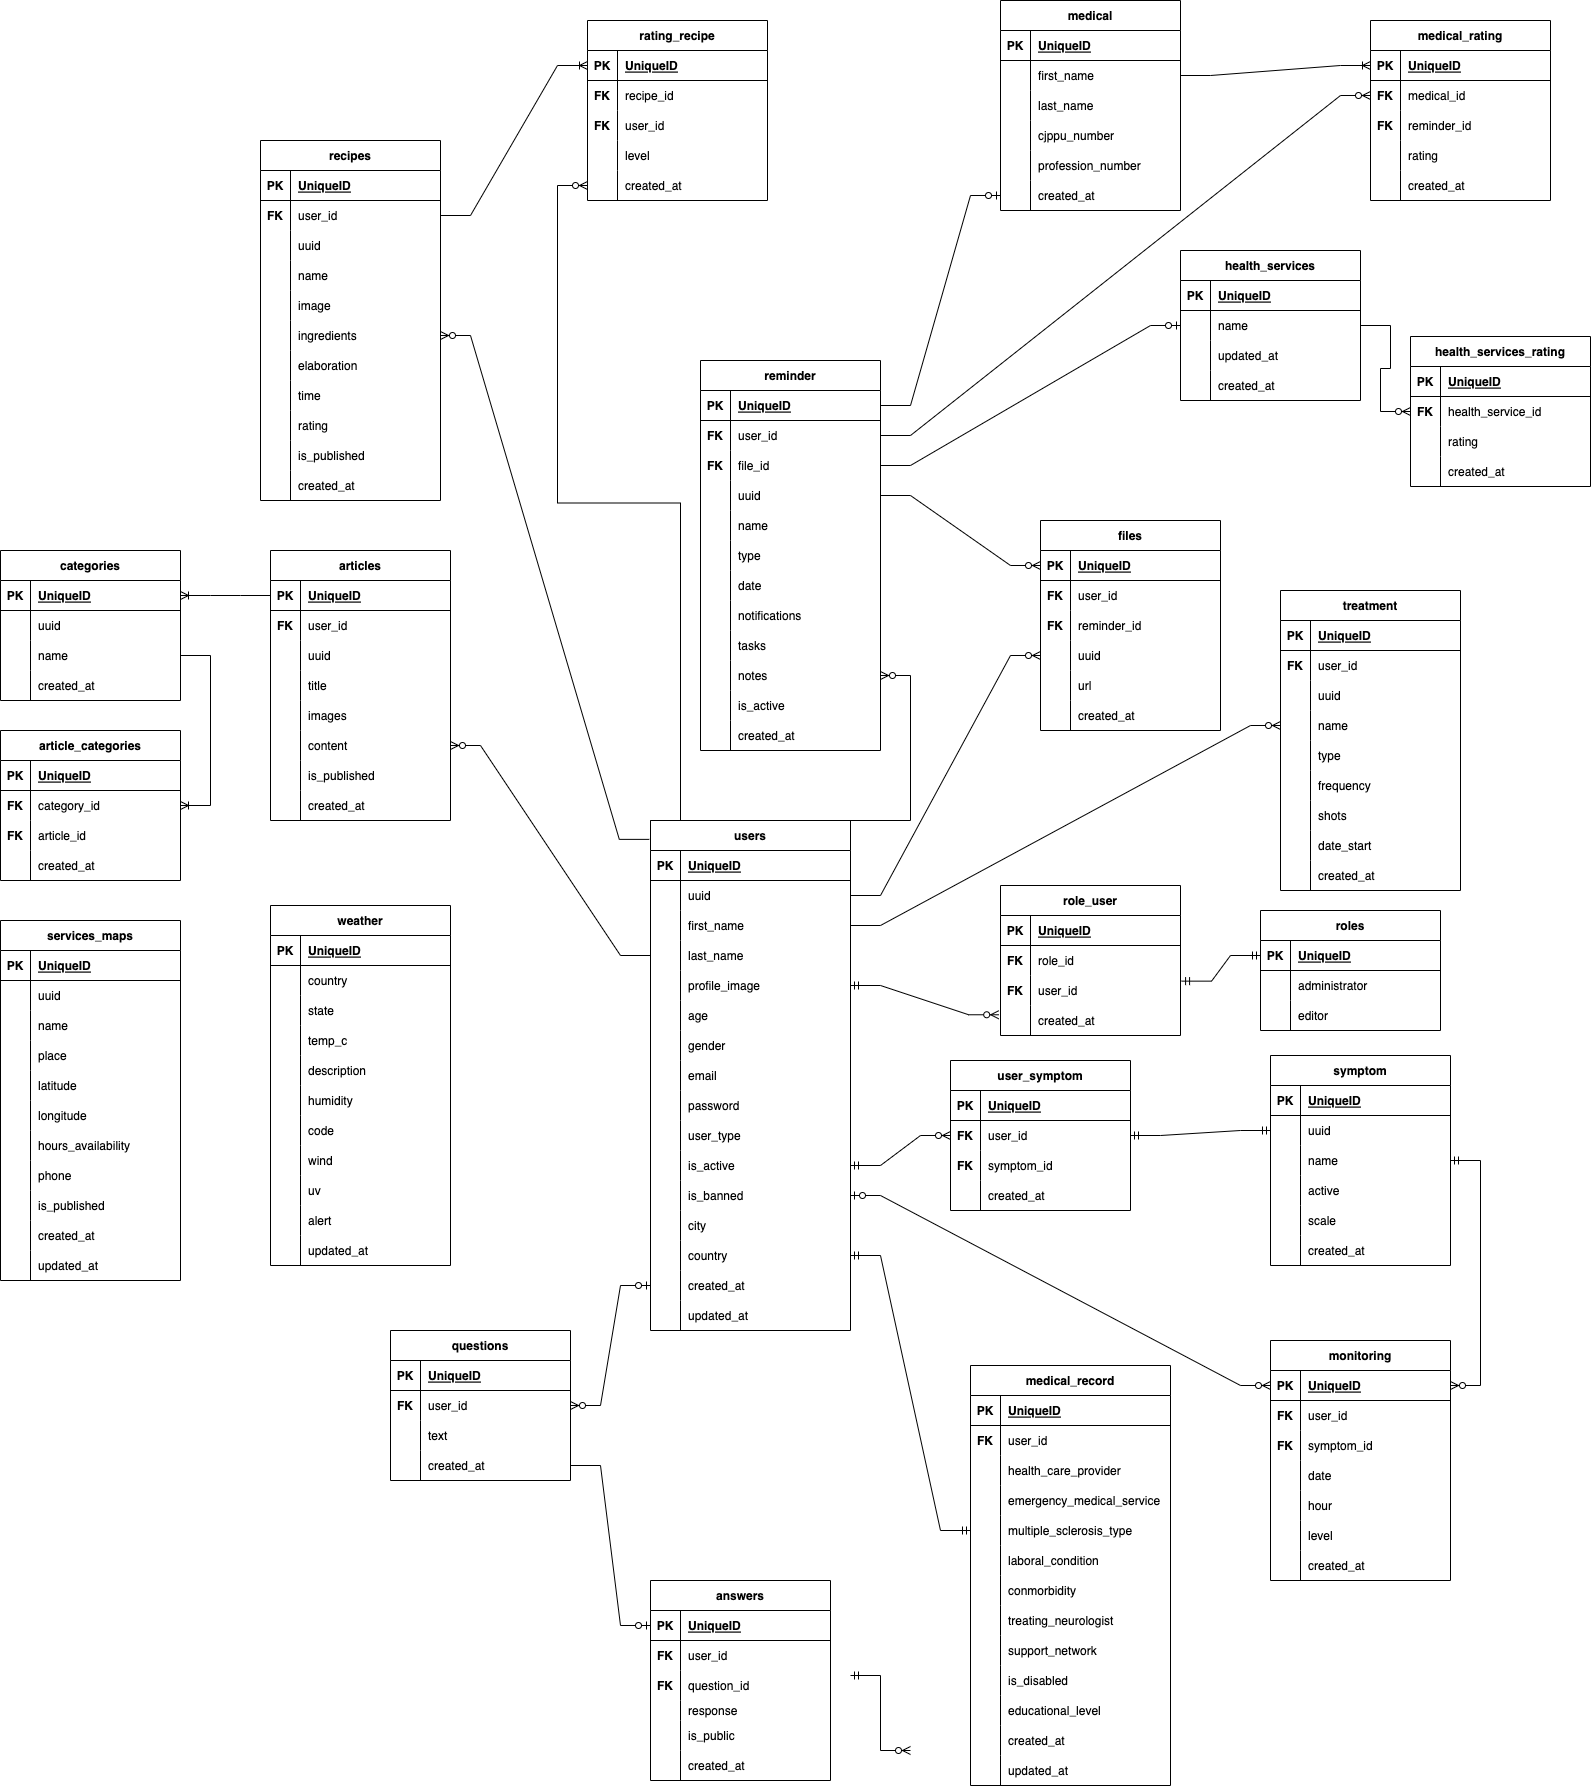
\includegraphics[width=0.7\textwidth]{img/datos/diagrama_db_backend.png}
    \caption{Diagrama MER del backend} \label{Img:Diseno+de+Datos+Backend}
\end{figure} 

\begin{figure}[h]
    \centering
    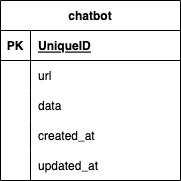
\includegraphics[width=0.3\textwidth]{img/datos/chatbot_emur.drawio.png}
    \caption{Diagrama de tabla para el chatbot} \label{Img:Diseno+de+Datos+Chatbot}
\end{figure} 

\newpage
\section{Diseño procedimental}
A propósito de la arquitectura hexagonal que se ha decidido implementar, se siguió un enfoque modular y basado en la  responsabilidad de cada componente, lo cual incluye controladores (capa de presentación), servicios y puertos que se encuentran en la capa de dominio; por último adaptadores de persistencia ubicados en la capa de datos (ver figura~\ref{Img:Diseno+Procedimental}), el documento original del diagrama también se puede ver en \href{https://drive.google.com/file/d/1Dp13RXxUGILHrhwLvSDbNNQ2T72sM4j7/view?usp=sharing}{draw.io}.

\begin{figure}[h]
    \centering
    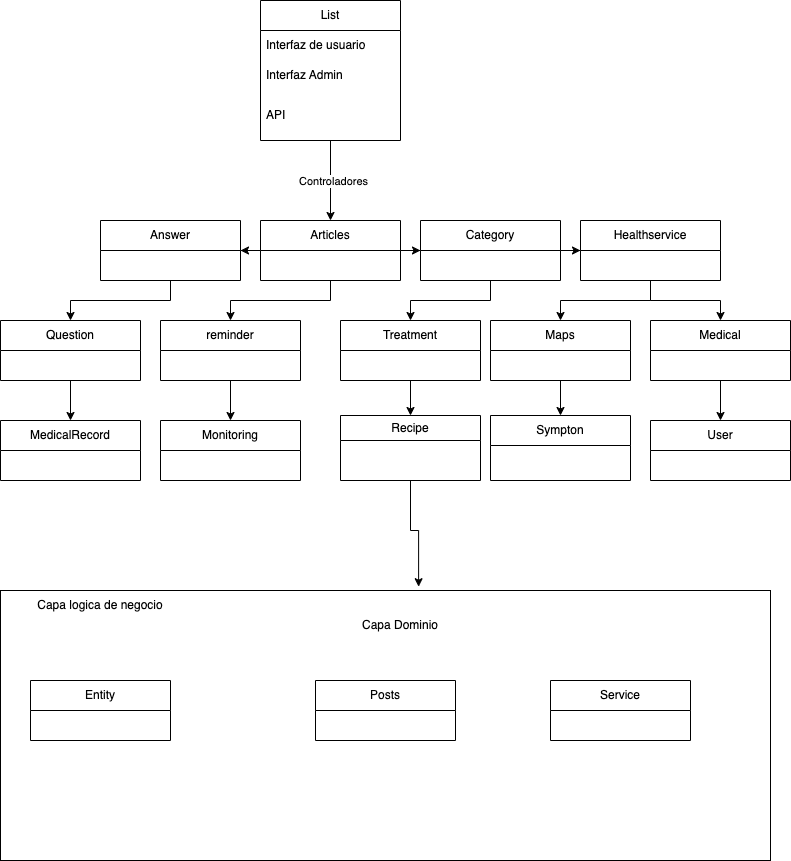
\includegraphics[width=0.7\textwidth]{img/manual/procidemental_drawio.png}
    \caption{Diseño Procedimental} \label{Img:Diseno+Procedimental}
\end{figure} 


\section{Diseño arquitectónico}
A continuación, se presenta la figura~\ref{Img:Diseno+Arquitectura}, donde se aprecia el diseño de arquitectura en el que es posible observar cómo se orquestan los microservicios del backend  y del chatbot para interactuar con la futura aplicación móvil.

\begin{figure}[h]
    \centering
    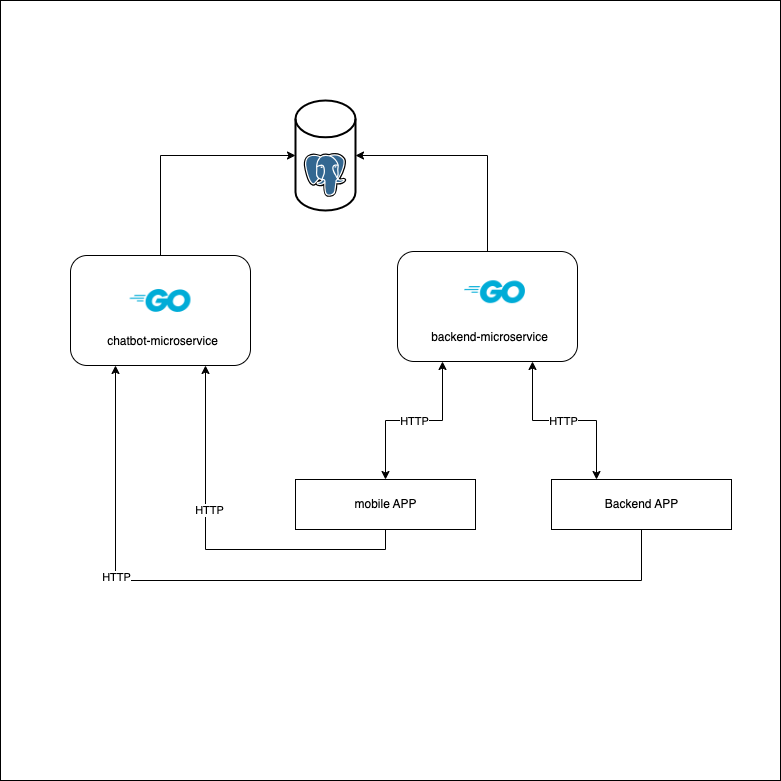
\includegraphics[width=1.0\textwidth]{img/datos/microservices-TFG.drawio.png}
    \caption{Diseño de Arquitectura} \label{Img:Diseno+Arquitectura}
\end{figure} 

\newpage

\section{Diseño de interfaces}

\subsection{Logo para la aplicación móvil a desarrollar a futuro}
Se ha elaborado un logo para la futura aplicación móvil utilizando Adobe Illustrator, conforme puede apreciarse en la figura~\ref{Img:Logo+APP}.

\begin{figure}[h]
    \centering
    
\includegraphics[width=0.4\textwidth]{img/app/red_em.png}
    \caption{Logo propuesto para la aplicación a desarrollar} \label{Img:Logo+APP}
\end{figure} 


\subsection{Interfaz de usuario para la futura aplicación móvil}
Durante la fase de diseño, se elaboraron bocetos digitales sobre cómo debería ser la futura aplicación móvil. Para este fin se utilizó la herramienta Marvel con el fin de poder prototipar las ideas, testearlas y simular su funcionamiento. Se pone a disposición una versión navegable en el siguiente \href{https://marvelapp.com/prototype/c69dgae}{enlace}.

A continuación, es posible observar los prototipos elaborados:

\begin{figure}[h]
    \centering
    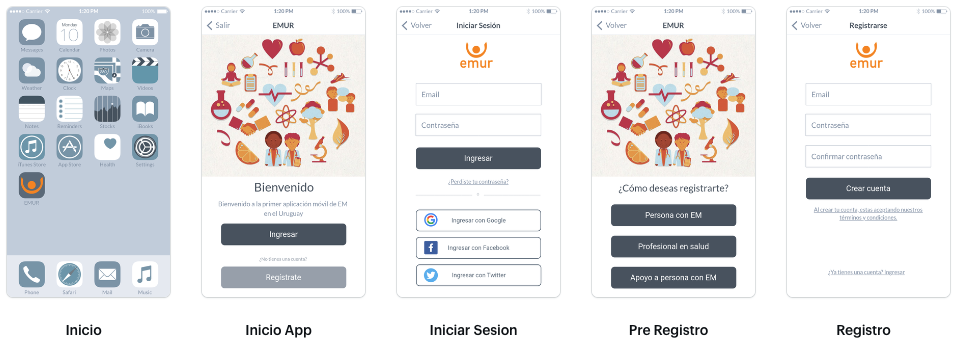
\includegraphics[width=1.1\textwidth]{img/app/diseno_parte1.png}
    \caption{Inicio y Registro} \label{Img:Inicio+Registro}
\end{figure} 

\begin{figure}[h]
    \centering
    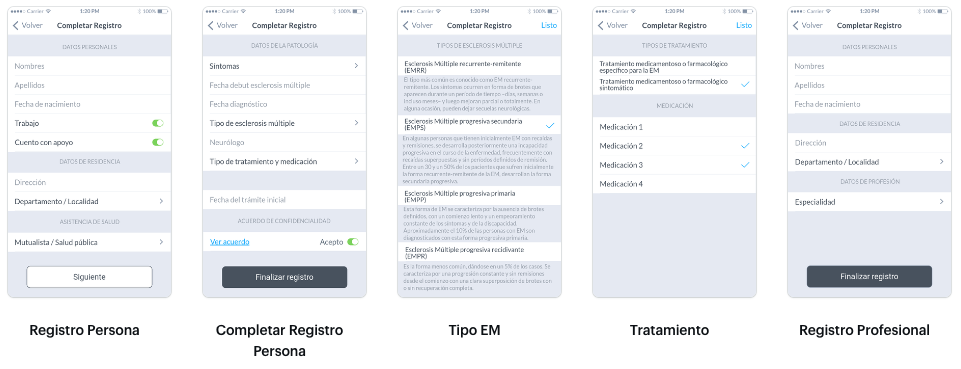
\includegraphics[width=1.1\textwidth]{img/app/diseno_parte2.png}
    \caption{Formularios de Registro} \label{Img:Formularios+Registro}
\end{figure} 

\begin{figure}[h]
    \centering
    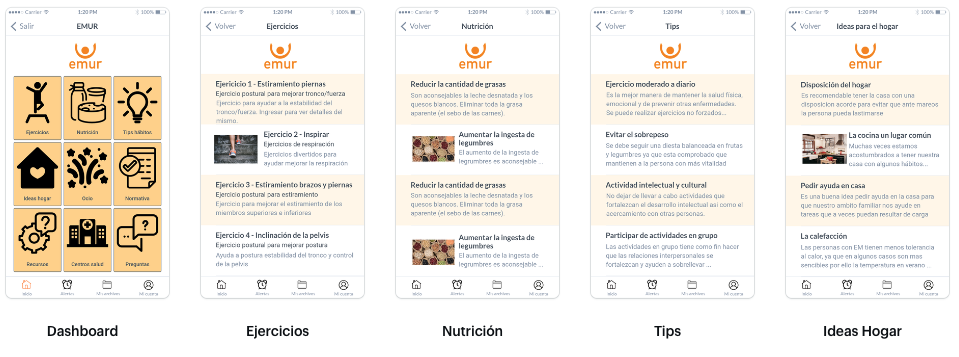
\includegraphics[width=1.1\textwidth]{img/app/diseno_parte3.png}
    \caption{Menú principal y tipos de artículos} \label{Img:Menu+articulos}
\end{figure} 

\begin{figure}[h]
    \centering
    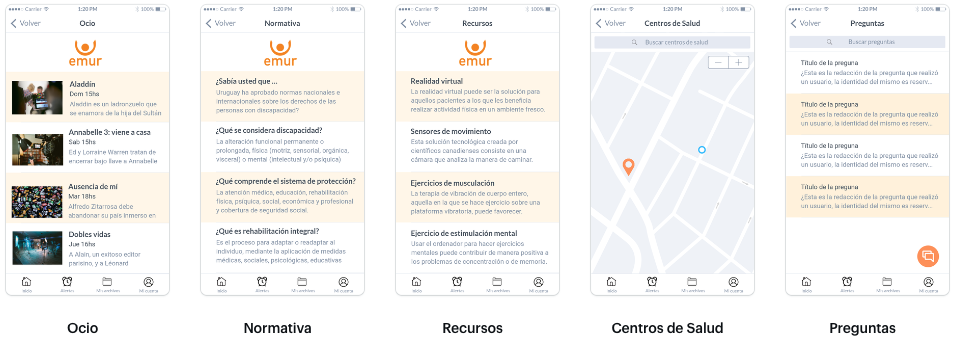
\includegraphics[width=1.1\textwidth]{img/app/diseno_parte4.png}
    \caption{Mapa, Recursos, Vista general de preguntas} \label{Img:Mapa+Recursos}
\end{figure} 

\begin{figure}[h]
    \centering
    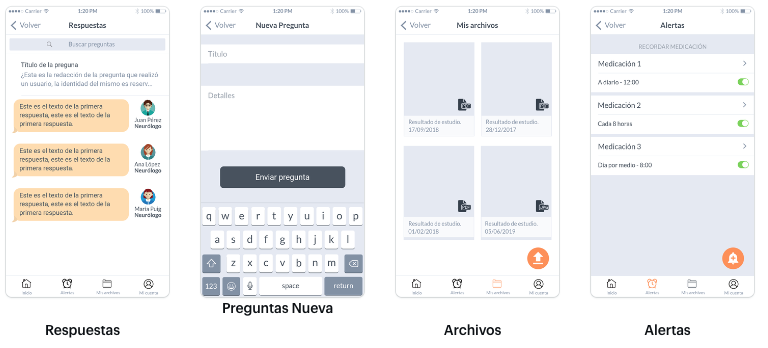
\includegraphics[width=1.1\textwidth]{img/app/diseno_parte5.png}
    \caption{Preguntas y Respuestas, Alertas y Gestión de archivos} \label{Img:Preguntas+Respuestas}
\end{figure} 
\apendice{Documentación técnica de programación}
\section{Introducción}
El manual de programador es una herramienta esencial para cualquier profesional que se dedique al desarrollo de software. Su objetivo principal es proporcionar información detallada y clara sobre el uso de un programa o aplicación, así como guías y recomendaciones para la resolución de problemas y situaciones que puedan surgir durante el proceso de programación.

Así, este manual le permitirá al programador ahorrar tiempo al consultar rápidamente la información necesaria en lugar de tener que buscarla en diferentes fuentes, así como también reducir los errores y los problemas de compatibilidad, ya que proporciona una guía clara sobre el uso adecuado de las herramientas y los recursos disponibles. De igual forma, permite optimizar la calidad del software desarrollado, ilustrando sobre las mejores prácticas y los estándares de calidad que deben seguirse durante el proceso de programación. 

Tal es el caso del presente Manual de Programador en el que se indican los pasos a seguir para el despliegue del backend desarrollado en este TFG que dará lugar a la futura aplicación móvil, dirigida a personas afectadas por la EM, en su intención de ayudarles a navegar por el sistema de salud y autogestionar su enfermedad desde el momento en que son diagnosticadas.

En este sentido, a continuación, se explican las diferentes etapas para el despliegue del backend en un servidor, así como también las herramientas con las que se deberá trabajar para realizar cualquier tipo de mantenimiento o desarrollar nuevas funcionalidades.

\subsection{Infraestructura}\label{infraestructura}
El backend debe estar alojado en un servidor web. En este caso se seleccionó Digital Ocean.

Digital Ocean es una plataforma de alojamiento en la nube que ofrece la posibilidad de crear y administrar maquinas virtuales, en adelante Droplets, así como otros servicios relacionados con la infraestructura en la nube; proporciona un entorno seguro y escalable para la implementación de aplicaciones web y móviles \cite{web:docker}.

\subsubsection{Creación de cuenta}
 El primer paso a seguir para utilizar la plataforma es el registro y creación de usuario. Para ello debemos dirigirnos al sitio web de la plataforma ingresando al siguiente enlace: \href{https://www.digitalocean.com/}{Digital Ocean}.

Una vez dentro del sitio, y encontrándose en la página de inicio, se debe hacer clic en la opción de Sign Up (Registrarse, en español), ubicada en la parte derecha de la misma. Está opción nos llevará a la sección donde nos registramos utilizando nuestro correo electrónico (ver figura~\ref{Img:Web+Digital+Ocean}).

\begin{figure}[h]
    \centering
    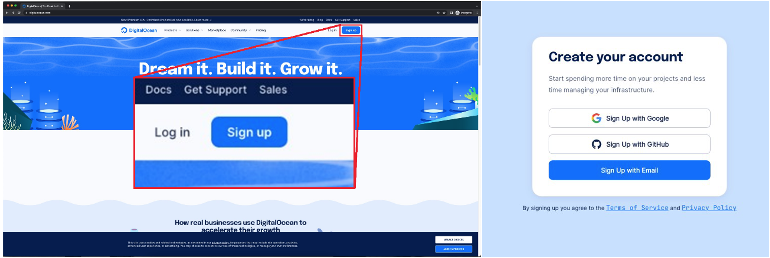
\includegraphics[width=0.9\textwidth]{img/infraestructura/pagina_digital_ocean.png}
    \caption{Creación de usuario en DigitalOcean.} \label{Img:Web+Digital+Ocean}
\end{figure}

Se debe hacer clic en la tercera opción marcada en azul, Sing Up with email, la que nos permitirá ingresar con un usuario y correo sin necesidad de usar sistemas de Single Sign On, como lo son Google o Github (ver figura~\ref{Img:Web+Registro+en+Digital+Ocean}).

\begin{figure}[h]
    \centering
    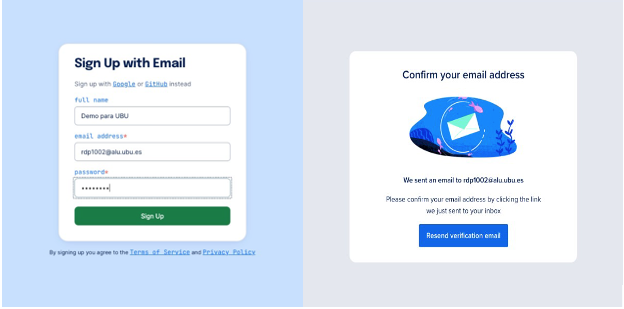
\includegraphics[width=0.9\textwidth]{img/infraestructura/pagina_de_registro.png}
    \caption{Registro y confirmación de email.} \label{Img:Web+Registro+en+Digital+Ocean}
\end{figure} 

\newpage

Una vez que rellenamos los datos que nos solicita la plataforma, ésta nos enviará un código de confirmación por email para comprobar que hemos sido nosotros quienes creamos la cuenta (ver figura~\ref{Img:Web+Registro+en+Digital+Ocean}). En este punto tendremos que abrir nuestro correo electrónico en la plataforma que corresponda, acceder al mail que hayamos recibido de Digital Ocean para verificar nuestra identidad, y luego hacer clic en el enlance que se nos suministra para confirmar la cuenta.\\
Habiendo completado el paso anterior, la plataforma nos solicitará dar de alta una tarjeta de crédito, o asociar una cuenta de Paypal, para poder realizar los pagos mensuales correspondientes al uso del servicio. Además, es importante destacar que Digital Ocean solicita realizar una recarga inicial de 5, 10 o 20 dólares americanos para poder comenzar a utilizar los servicios; una vez realizado este pago la plataforma cobrará a mes vencido.

\subsubsection{Creación de Droplet}

Luego de completar el registro e iniciar sesión en la plataforma, pasamos a la creación del Droplet. Un Droplet es un servidor virtual independiente que se puede configurar para realizar una variedad de tareas; es una combinación de recursos informáticos, como RAM, CPU y almacenamiento, que se pueden escalar vertical u horizontalmente según las necesidades del usuario \cite{web:digitalocean}. Por otra parte, un servidor virtual es un software que simula el hardware de una computadora y permite que múltiples sistemas operativos compartan los recursos de una sola máquina física \cite{web:vps}.

Así, en Digital Ocean las instancias de máquinas virtuales son llamadas Droplet, y cada una tiene ciertas características de acuerdo con el propósito con el que se utilizará el mismo. En nuestro caso, usaremos un Droplet de propósito general, con un costo de 7 dólares por mes, para comenzar a trabajar dado que permite escalar el sistema en un futuro, si lo necesitamos. Asimismo, el Droplet de propósito general ofrece una amplia gama de opciones de configuración. Para crear el Droplet, seguiremos los pasos descriptos a continuación. 

Estando dentro de nuestro perfil en Digital Ocean, hacemos clic en la opción Create, en la parte superior derecha, y luego seleccionamos la opción Droplets que nos llevará a la siguiente sección en donde debemos elegir la zona geográfica, sistema operativo y el tipo de Droplet a crear (ver figura~\ref{Img:Web+Creación+de+droplet+en+Digital+Ocean}). 

\begin{figure}[h]
    \centering
    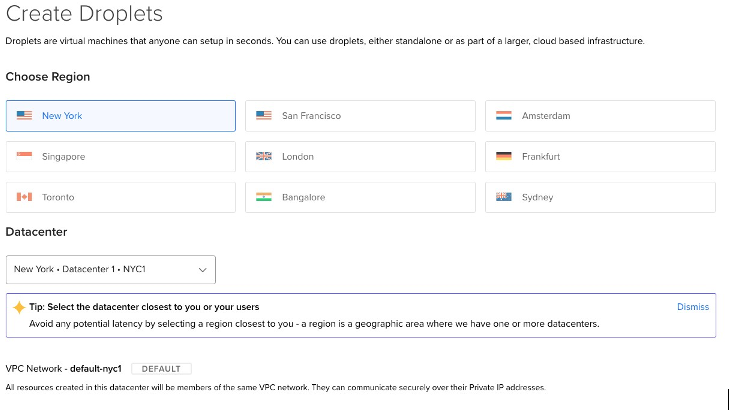
\includegraphics[width=0.9\textwidth]{img/infraestructura/crear-droplet.png}
    \caption{Crear droplet} \label{Img:Web+Creación+de+droplet+en+Digital+Ocean}
\end{figure} 

En nuestro caso, hemos seleccionado Nueva York (por tratarse del área más cercana a Latinoamérica) y, en lugar de trabajar con una máquina con el sistema operativo, hemos seleccionado desde el Marketplace una imagen precreada de Docker, que integra también Docker Compose.

Lo anterior responde a un uso inteligente de los recursos existentes para evitar instalar Docker manualmente y evitar posibles fallos durante dicho proceso.

Amerita explicitar que Docker es una plataforma de software que permite la creación, el despliegue y la ejecución de aplicaciones en contenedores, mientras que un contenedor es un ambiente de software que ofrece todo lo necesario para ejecutar una aplicación, incluyendo el código, las bibliotecas y las herramientas del sistema \cite{web:docker}. Por otro lado, Docker Compose es una herramienta que permite definir y ejecutar aplicaciones Docker compuestas por múltiples contenedores \cite{web:docker-compose}. 

\subsubsection{Creación de SSH KEY}

En lo referente a la seguridad, se puede establecer que, para acceder al Droplet, se deba utilizar bien sea una contraseña o una llave SSH KEY, siendo esta última opción la utilizada. Una SSH KEY es una clave criptográfica utilizada para autenticación y encriptación en la comunicación segura a través del protocolo SSH, referido al acceso a un servidor mediante el uso de un canal seguro que permite a un usuario autenticarse en un servidor remoto, sin tener que ingresar una contraseña cada vez que se inicia sesión \cite{web:ssh-key}.

Para agregar una SSH KEY a Digital Ocean seleccionamos esta opción cuando creamos el Droplet marcando New SSH KEY en la sección Choose authentication method. En este punto, se nos desplegará un modal que nos permitirá agregar nuestra SSH Key personal, la que debemos haber creado previamente (ver figura~\ref{Img:Web+Método+de+autenticación+SSH+KEY}).


\begin{figure}[h]
    \centering
    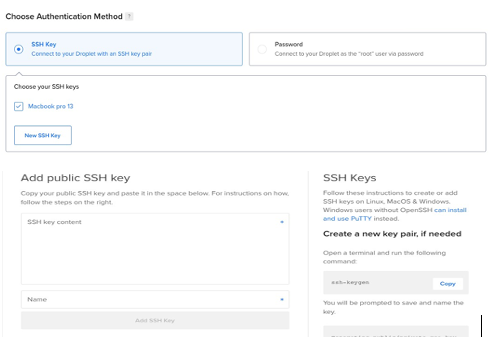
\includegraphics[width=0.8\textwidth]{img/infraestructura/ssh-key.png}
    \caption{Método de autenticación SSH KEY} \label{Img:Web+Método+de+autenticación+SSH+KEY}
\end{figure} 


Si en nuestra computadora no tenemos una clave generada previamente del tipo SSH KEY procederemos a generarla abriendo la terminal de comandos en el sistema operativo. En el caso de las computadoras MAC con sistema operativo OSX, para abrir la terminal se debe presionar el atajo de teclado cmd + barra espaciadora. Luego, debemos ingresar el siguiente comando: ssh-keygen, y enseguida la consola preguntará si le queremos dar un nombre y si se desea agregar una contraseña a la llave (ver figura~\ref{Img:Creación+de+SSH+KEY+en+MAC}).

\begin{figure}[h]
    \centering
    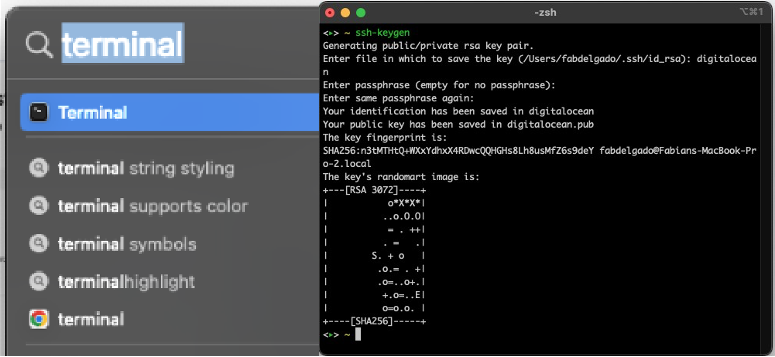
\includegraphics[width=0.8\textwidth]{img/infraestructura/crear-ssh-key-mac.png}
    \caption{Creación de SSH KEY en MAC} \label{Img:Creación+de+SSH+KEY+en+MAC}
\end{figure} 


Una vez finalizado este proceso, debemos copiar la llave generada en Digital Ocean, para lo cual nos dirigimos al directorio donde se guardan todas las llaves: cd/Users/fabdelgado/.ssh/. Una vez en el directorio, ejecutamos el comando “ls” para ver todas las llaves generadas y encontrar la que necesitamos. Luego, para copiar la clave generada ejecutamos el comando “cat digitalocean.pub” (ver figura~\ref{Img:Copiado+de+clave+generada}). Es de tener en cuenta que se debe realizar con la llave en la extension .pub por ser ésta la clave pública.

\begin{figure}[h]
    \centering
    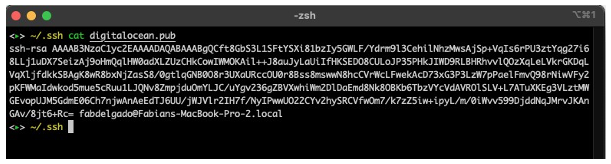
\includegraphics[width=0.7\textwidth]{img/infraestructura/copiado-ssh-key.png}
    \caption{Copiado de clave generada.} \label{Img:Copiado+de+clave+generada}
\end{figure} 

Una vez copiado el contenido de la clave pública procedemos a ingresarla en la cuenta de Digital Ocean y darle un nombre para guardarla en la plataforma. Finalmente, presionamos Add SSH Key y de esta forma ya nos queda disponible para futura creación de otros Droplets (ver figura~\ref{Img:Agregar+SSH+KEY+en+DigitalOcean}).

\newpage
\begin{figure}[h]
    \centering
    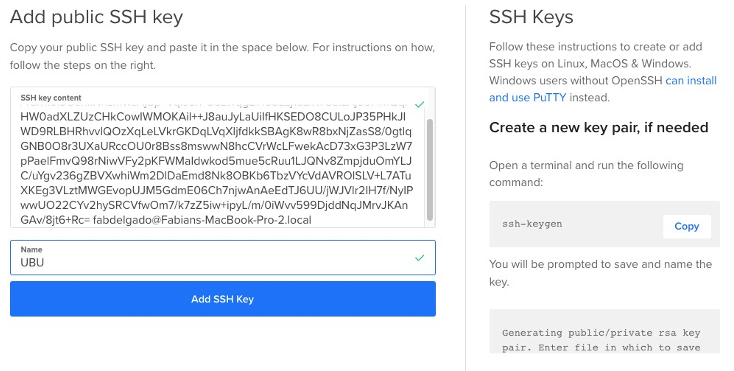
\includegraphics[width=0.7\textwidth]{img/infraestructura/agregar-ssh-key-digital-ocean.png}
    \caption{Agregar SSH KEY en DigitalOcean.} \label{Img:Agregar+SSH+KEY+en+DigitalOcean}
\end{figure} 


\subsubsection{Creación de base de datos}
Para la creación de la base de datos también se utiliza un servicio ofrecido por Digital Ocean a este respecto. Ello brinda alta disponibilidad y permite despreocuparnos del mantenimiento y los respaldos diarios a realizar.
Para crear una nueva instancia de base de datos se hace clic en el botón Create, y se selecciona la opción Databases, que redirige a una página para establecer la configuración de la instancia que deseamos crear. En nuestro caso seleccionamos la región por defecto de Nueva York para tener menos latencia con el Droplet previamente creado, y como motor de base de datos seleccionamos PosgretSQL en el plan starter (ver figura~\ref{Img:Creación+de+base+de+datos en+DigitalOcean}).
\begin{figure}[h]
    \centering
    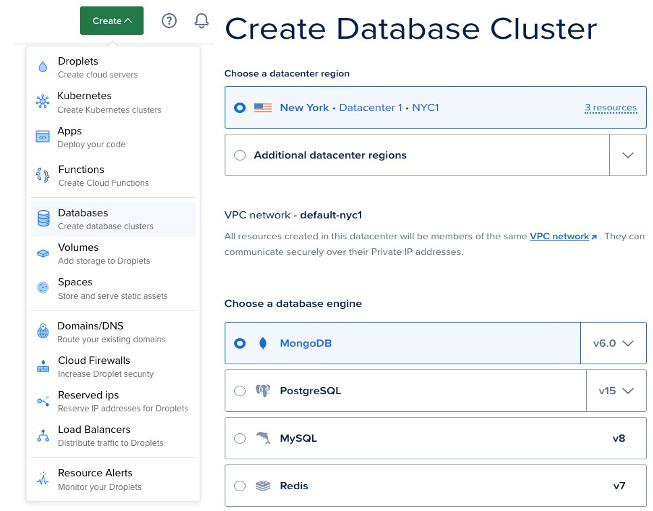
\includegraphics[width=0.6\textwidth]{img/infraestructura/crear-base-de-datos.png}
    \caption{Creación de base de datos en DigitalOcean.} \label{Img:Creación+de+base+de+datos en+DigitalOcean}
\end{figure} 


En relación con lo anterior, PostgreSQL es un sistema de gestión de bases de datos ORDBMS (Object-Relational Database Management System) de código abierto y de alta performance, que utiliza un modelo cliente-servidor, siendo, además, altamente escalable. PostgreSQL posee una arquitectura modular, lo que significa que los módulos pueden ser añadidos o eliminados a medida que las necesidades van mutando \cite{web:postgresql}.
Para finalizar, debemos indicar el nombre que deseamos colocar para la instancia, y seleccionar el proyecto al que queremos que esté relacionado, que en este caso es el llamado EMUR. Así, luego de confirmar la creación, ya nos aparece en nuestro panel de proyecto, siendo el siguiente paso la creación del usuario con el que nos conectaremos a la base de datos donde se guarda la información. 
En este sentido, para configurar el usuario y la base de datos debemos dirigirnos al apartado Users and Databases, en el que crearemos un usuario llamado EMUR, una base de datos para desarrollo y una para producción llamada Backend (ver figura~\ref{Img:Configuración+de+usuario+en PostgreSQL}).

\begin{figure}[h]
    \centering
    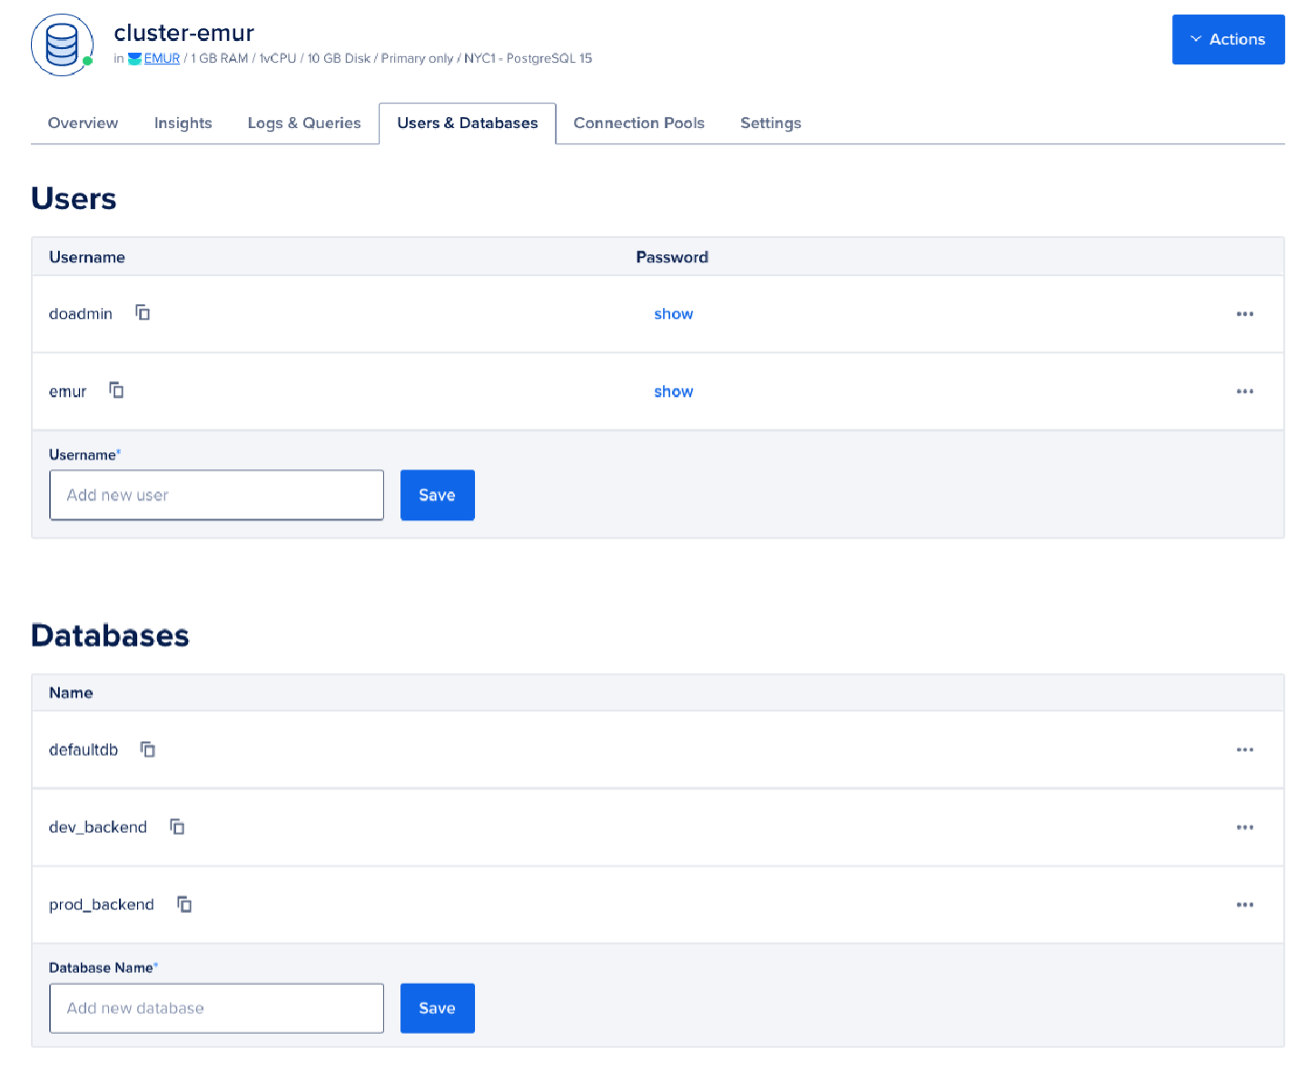
\includegraphics[width=0.9\textwidth]{img/infraestructura/cluster-db-digital-ocean.png}
    \caption{Configuración de usuario en PostgreSQL.} \label{Img:Configuración+de+usuario+en PostgreSQL}
\end{figure} 


\subsection{}{SonarQube}

SonarQube es una herramienta de análisis estático de código que permite detectar problemas y vulnerabilidades en el código fuente; es una herramienta efectiva para medir la calidad del código que proporciona una gran cantidad de métricas que permiten evaluar la complejidad, legibilidad y mantenibilidad del código \cite{web:sonarqube}. En este sentido, luego de realizar una análisis comparativo de costos, contrastando el costo de tener un servidor dedicado para utilizar SonarQube contra la opción de usar la versión hosteada por SonarQube, se decide optar por la versión en la nube de SonarCloud de más bajo coste (ver tabla~\ref{tab:requisitos-sonar}).

\begin{table}[H]
\centering
\begin{tabular}{ll}
\toprule
Plataforma                     & Precio                           \\
\midrule
\texttt{Digital Ocean SonarQube}       & 12 USD              \\
\texttt{SonarQube Cloud}      & 10 USD             \\
\bottomrule
\end{tabular}
\caption{Comparativa de precios SonarQube}
\label{tab:requisitos-sonar}
\end{table}

Para crear el usuario en SonarCloud se utiliza el Single Sign On de Github que condice con el hecho de que nuestro proyecto se encuentra en esta plataforma y nos resultará más fácil su integración.\\

Para crear un proyecto en SonarCloud debemos de usar la opción Import an organization from GitHub (ver figura~\ref{Img:Registro+en+SonarCloud}).
\begin{figure}[h]
    \centering
    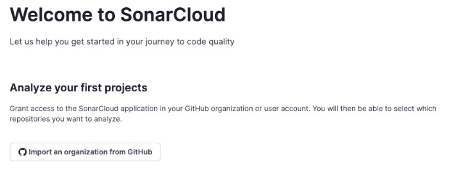
\includegraphics[width=0.9\textwidth]{img/infraestructura/registro-sonarcloud.png}
    \caption{Registro en SonarCloud.} \label{Img:Registro+en+SonarCloud}
\end{figure} 

Luego de esto, el siguiente paso será seleccionar la organización a sincronizar, en este caso EMUR-UY, para después indicar si vamos a otorgar permisos sobre todos los repositorios o sólo algunos. Para el caso que nos convoca, seleccionaremos Only select repositories, lo cual nos permite tener un control más detallado sobre los proyectos que queremos importar para analizar, y por último pulsamos Install (ver figura~\ref{Img:Configuracion+de+SonarCloud}).

\begin{figure}[h]
    \centering
    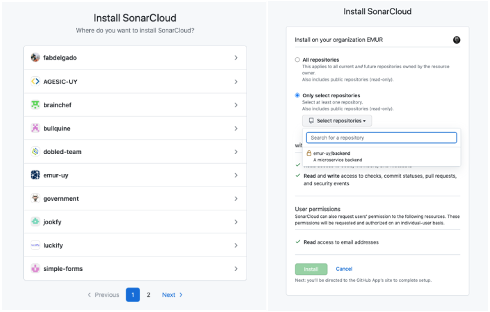
\includegraphics[width=0.9\textwidth]{img/infraestructura/configurar-sonar-cloud.png}
    \caption{Configuracion de SonarCloud.} \label{Img:Configuracion+de+SonarCloud}
\end{figure} 
\newpage

Seguidamente, SonarCloud, nos solicita crear una organización (ver figura~\ref{Img:Crear+organización}), donde nos pide ingresar email, identificador de proyecto y tipo de plan, para después solicitar la información de pago y el tipo de uso, y así proceder con la creación del proyecto. 

\begin{figure}[h]
    \centering
    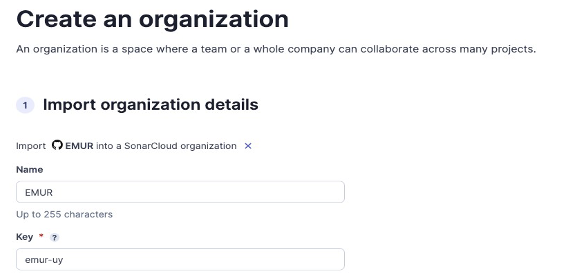
\includegraphics[width=0.7\textwidth]{img/infraestructura/crear-organizacion.png}
    \caption{Crear organización.} \label{Img:Crear+organización}
\end{figure} 

Tras realizar todas estas precisiones procedemos a configurar el proyecto que necesitamos escanear haciendo clic en Set Up, con lo que SonarCloud comenzará a analizar todo el repositorio (ver figura~\ref{Img:Configuración+de+análisis+de+proyectos}).

\newpage
\begin{figure}[h]
    \centering
    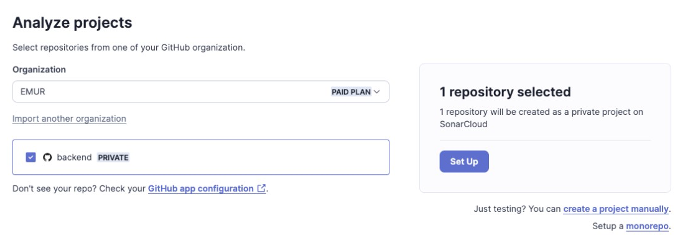
\includegraphics[width=0.7\textwidth]{img/infraestructura/configurar-proyecto.png}
    \caption{Configuración de análisis de proyectos.} \label{Img:Configuración+de+análisis+de+proyectos}
\end{figure} 


Una vez finalizado el análisis primario podemos observar que nos arroja la calidad del código (ver figura~\ref{Img:Resultado+de+análisis+de+código}).

\begin{figure}[h]
    \centering
    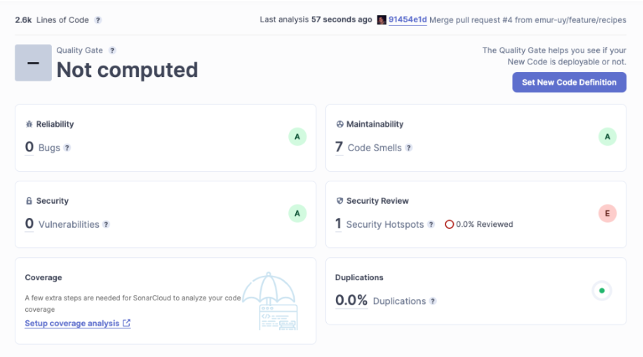
\includegraphics[width=0.7\textwidth]{img/infraestructura/calidad-de-codigo.png}
    \caption{Resultado de análisis de código.} \label{Img:Resultado+de+análisis+de+código}
\end{figure} 

Como podemos ver a continuación nuestro código ha pasado el análisis correctamente y apareciamosque no tiene bugs, ni vulnerabilidades, un bajo porcentaje de code smells y una salud satisfactoria en cuanto a seguridad (ver figura~\ref{Img:Calidad+del+codigo} y ver figura~\ref{Img:Calidad+del+codigo_2}).

\begin{figure}[h]
    \centering
    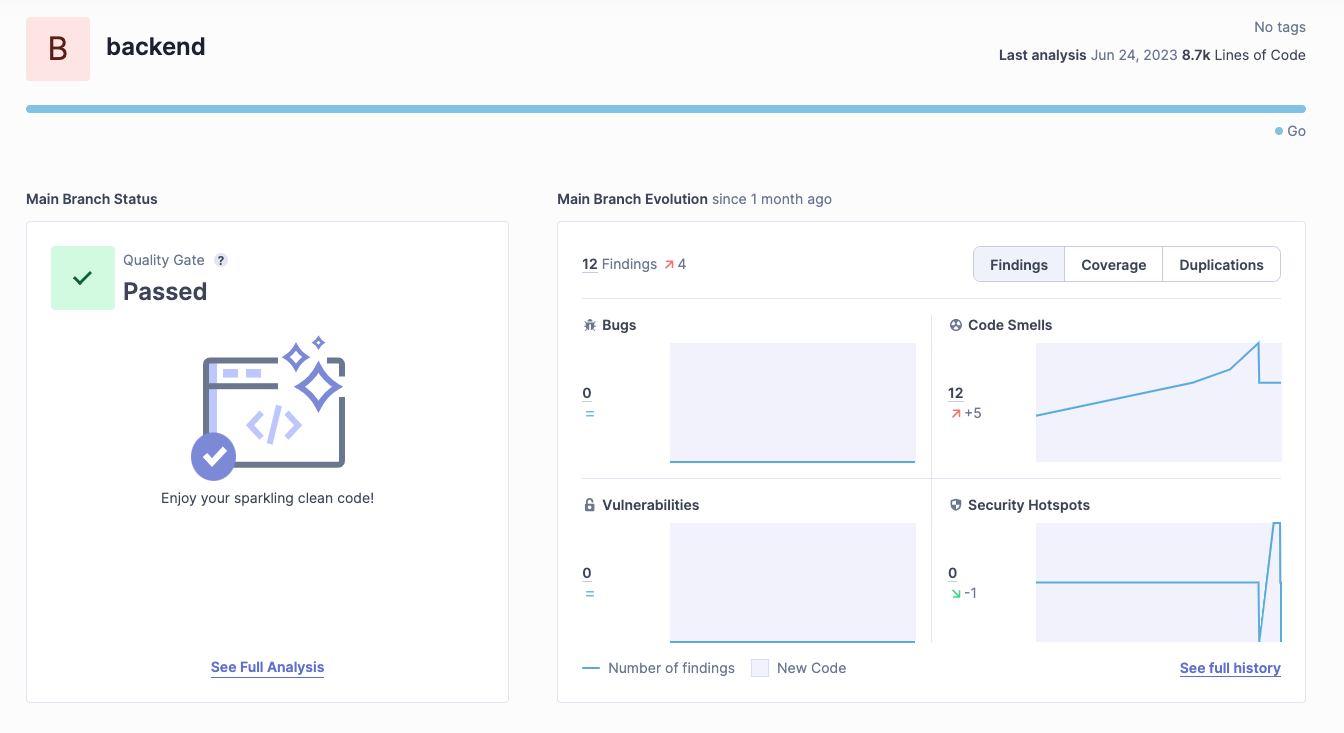
\includegraphics[width=0.8\textwidth]{img/manual/code_sonar_1.png}
    \caption{Resultado de calidad del código parte 1.} \label{Img:Calidad+del+codigo}
\end{figure} 

\begin{figure}[h]
    \centering
    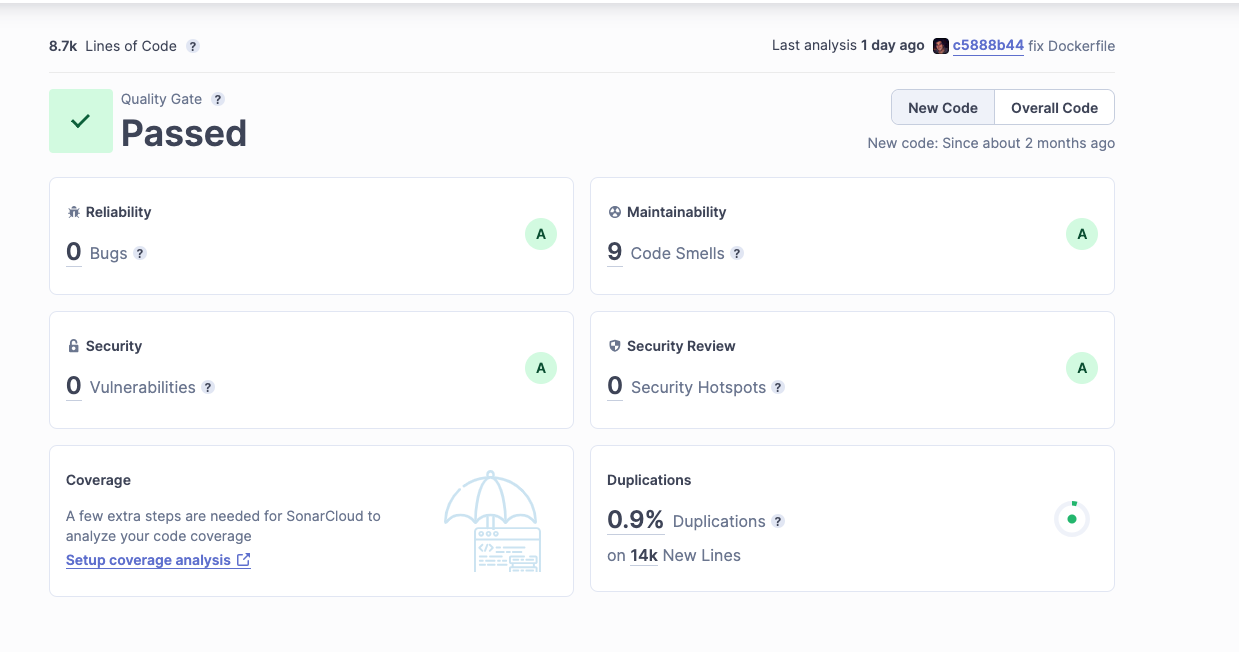
\includegraphics[width=0.8\textwidth]{img/manual/code_sonar.png}
    \caption{Resultado de calidad del código parte 2} \label{Img:Calidad+del+codigo_2}
\end{figure} 

Asimismo se puede ingresar al siguiente enlace para comprobar la calidad del código \href{https://sonarcloud.io/project/overview?id=emur-uy_backend}{SonarCloud}.
\newpage

\section{Github Actions}
Mediante el uso de esta herramienta podemos contar con un servicio de entrega continua, lo que permite subir el código a nuestro repositorio y Github, automáticamente, ejecuta los pipelines desplegando los cambios directamente en el servidor.

En este caso, la receta creada de actions, genera una imagen de Docker y la publica en el repositorio de Docker Hub, seguidamente se conecta al servidor para realizar el despliegue de la nueva imagen de Docker \href{https://hub.docker.com/repository/docker/fabdelgado/api-backend-emur}{Backend} y \href{https://hub.docker.com/repository/docker/fabdelgado/api-chatbot-emur/general}{Chatbot}.

Es de notar que actions de Github necesita ciertas configuración en el repositorio de forma de que pueda conectarse al servidor y al repositorio de Docker Hub, para ello en la sección de settings, en el aparato de seguridad existe una opcion llamada Actions secrets and variables, y es aquí donde procederemos a cargar las variables requeridas (ver tabla~\ref{tab:requisitos-actions}).

\begin{table}[H]
\centering
\begin{tabular}{ll}
\toprule
Variable                     & Valor                           \\
\midrule
\texttt{SERVER\_HOST}       & 134.209.128.98              \\
\texttt{SERVER\_USER}      & root             \\
\texttt{SERVER\_PASSWORD}      & jGqdvXlX2O             \\
\texttt{DEPLOY\_TOKEN}      & Llave pública del servidor             \\
\texttt{DOCKER\_USERNAME}      &  Usuario de Docker Hub      \\
\texttt{DOCKER\_PASSWORD}      & Clave de Docker Hub                \\
\bottomrule
\end{tabular}
\caption{Datos necesarios para Github Actions}
\label{tab:requisitos-actions}
\end{table}

Seguidamente se muestran los pipelines de Github Actions ejecutando las tareas de integración continua sobre el servidor para el backend (ver figura~\ref{Img:Github+Actions+Backend}) y el chatbot (ver figura~\ref{Img:Github+Actions+Chatbot}).

\begin{figure}[h]
    \centering
    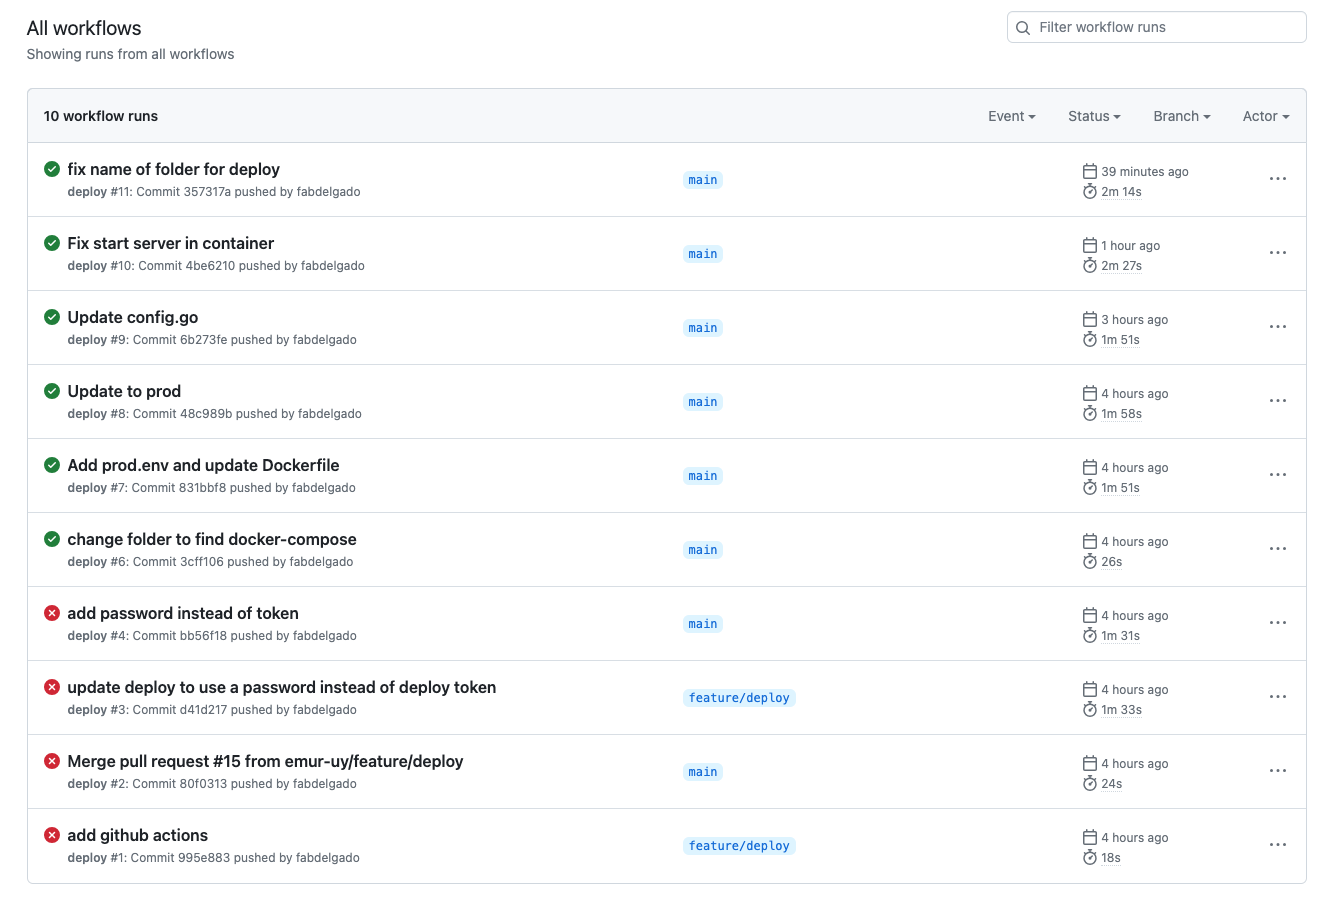
\includegraphics[width=0.7\textwidth]{img/github/ci_backend.png}
    \caption{Ejecución de Github Actions del backend} \label{Img:Github+Actions+Backend}
\end{figure} 

\begin{figure}[h]
    \centering
    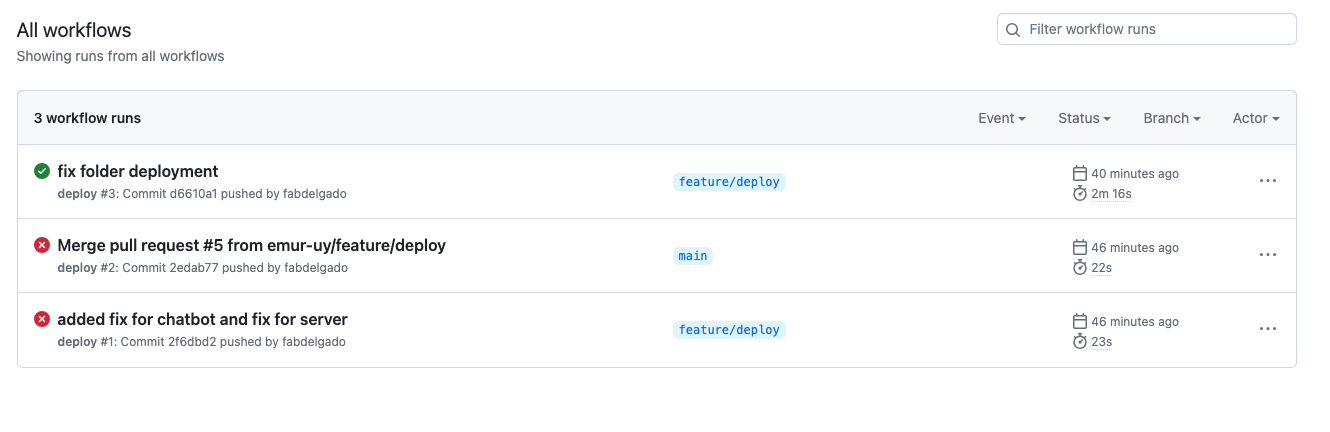
\includegraphics[width=0.7\textwidth]{img/github/ci_chatbot.png}
    \caption{Ejecución de Github Actions del chatbot} \label{Img:Github+Actions+Chatbot}
\end{figure} 

\newpage
\section{Estructura de directorios}

\subsection{Backend}
En el caso de este proyecto de backend la estructura de directorios es muy importante ya que permite organizar el código discriminando en base a las responsabilidades que tiene el sistema desarrollado y a cómo se estructura para mejorar la mantenibilidad en el futuro.

Esta sección detalla cómo está formada la estructura de directorios.

\begin{itemize}
\tightlist
\item
  \texttt{/}: directorio raíz del backend
  \begin{itemize}
  \tightlist
  \item 
    \texttt{makefile}: Archivo utilizado mediante el uso de make para generar las migraciones y ejecutar la creación de las tablas en la base de datos. 
  \item 
    \texttt{run test}: Script que tiene como finalidad la ejecución de los test unitarios.
  \item 
   \texttt{readme}: Contiene la información relevante del proyecto que permite a otros programadores conocer información importante en cuanto al desarrollo.
   \item 
   \texttt{go.mod}: Se encuentran definidas las dependencias del proyecto.
    \item 
   \texttt{go.sum}: Contiene los hashes de cada dependencia para garantizar la integridad.
   \item 
   \texttt{.env}: Archivos donde se alojan las variables de entorno para cada ambiente.
\end{itemize}
\item
  \texttt{/cmd}: contiene los puntos de entrada a la aplicación:
  \begin{itemize}
  \tightlist
  \item 
    \texttt{/api}: Contiene el archivo main, necesario para inicilizar el servidor web. 
  \item  
    \texttt{/worker}: Contiene el archivo main, necesario para inicilizar trabajadores en segundo plano.
    \end{itemize}
    \item
  \texttt{/config}: Contiene un archivo llamado de igual forma que se encarga de cargar las variables que se encuentran en el archivo .env disponibilizándolas a la aplicación.
  \item
  \texttt{/internal}: Contiene los detalles técnicos que necesita la aplicación para funcionar externos a la lógica de negocio de la aplicación.
  \begin{itemize}
  \tightlist
  \item 
    \texttt{/api}: Contiene los controladores y las rutas necesarias para comunicar la aplicación con el afuera.
  \item  
    \texttt{/forecast}: Contiene la implementación para comunicarse con un servicio externo para obtener datos del clima.
  \item  
    \texttt{/repositories}: Contiene los archivos necesarios para realizar la comunicación con repositorios tales como base de datos, storage externo, entre otros.
  \begin{itemize}
  \tightlist
  \item 
    \texttt{/postgresql}: Contiene la implementación abstracta para desacoplar el sistema de la implementación de base de datos.
  \item  
    \texttt{/spaces}: Contiene la implementación para realizar subida, actualización y eliminación de archivos desde un storage externo.
    \end{itemize}
          \item  
    \texttt{/pkg}:
\begin{itemize}
  \tightlist
  \item 
    \texttt{/entity}: Contiene la definición de las entidades también llamadas modelo de dominio.
  \item  
    \texttt{/ports}: Esta carpeta contiene las interfaces necesitarias para interconectar el servicio con la base de datos.
  \item  
    \texttt{/services}: Contiene la lógica de negocio.
    \end{itemize}
    \end{itemize}
    \texttt{/migrations}: Contiene los archivos SQL para generar las tablas o actualizarlas.
    \end{itemize}

\subsection{Chatbot}
En el caso de la estructura de directorios para el chatbot, se trata de una estructura muy simple ya que está basada en ejecución de scripts. A continuación se detallan los archivos más importantes.

\begin{itemize}
\tightlist
\item
  \texttt{/}: directorio raíz del chatbot
  \begin{itemize}
  \tightlist
  \item 
    \texttt{alembic}: Contiene las migraciones para la base de datos.
  \item 
    \texttt{db\_docs}: Contiene la estructura generada por FAISS de vectores.
  \item 
   \texttt{api.py:}: Script que disponibiliza la API.
   \item 
   \texttt{engine.py:} Script motor que genera los vectores para FAISS a partir de la información extraída de la base de datos.
    \item 
    \texttt{chatbot.py:}Script que se encarga de buscar el vector mas cercano a la pregunta del usuario y interactuar con ChatGPT para generar la respuesta.
    \item 
    \texttt{scrapper.py:} Script encargado de navegar por el sitio web extrayendo y formateando la información en crudo para que luego se procesada por el engine.
   \item 
   \texttt{.env}: Archivos donde se alojan las variables de entorno para el ambiente.
    \item 
   \texttt{requirements.txt}: Se encuentran definidas las dependencias del proyecto .
    \item 
   \texttt{startup.sh}: Inicia el servidor gunicorn usando hilos.
    \end{itemize}
\end{itemize}

 
\section{Compilación, instalación y ejecución del proyecto}
Esta sección tiene como objetivo brindar los conocimientos básicos que permitan entender cómo trabajar con el proyecto, realizar modificaciones o evolucionarlo en el tiempo.

 \subsection{Entorno de desarrollo}
Es necesario contar con las siguientes herramientas aqui descriptas:
 
 \begin{itemize}
  \tightlist
  \item Visual Studio Code
  \item Golang
  \item Python
  \item Git
  \item Table Plus
  \item Postman
  \item Make
\end{itemize}

\subsubsection{Visual Studio Code}\label{visual-studio-code}

Visual Studio Code es un editor de código de fuente abierto, gratuito, y multiplataforma con una gran cantidad de extensiones disponibles, y que se utiliza para desarrollar aplicaciones en una variedad de lenguajes de programación como Python, JavaScript, TypeScript, Golang, entre otros. En este sentido, no se requirió de licencia para el editor de código facilitando su uso.

Para abrir el proyecto en Visual Studio Code primero debemos proceder a realizar la descarga de este software (ver figura~\ref{Img:Descarga+de+Visual+studio+code}).
Para ello nos dirigimos a la \href{https://code.visualstudio.com/}{web oficial}. 

\begin{figure}[h]
    \centering
    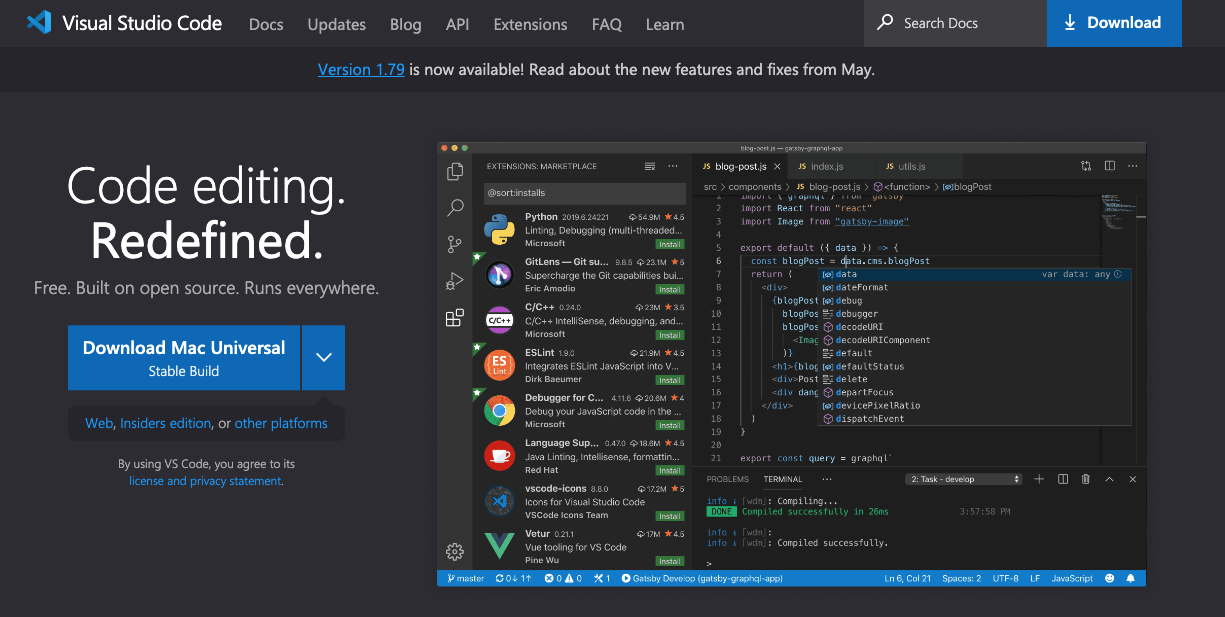
\includegraphics[width=0.7\textwidth]{img/manual/visual-studio-code.png}
    \caption{Descarga de Visual Studio Code} \label{Img:Descarga+de+Visual+studio+code}
\end{figure} 

Para instalarlo, basta con arrastrar el software hacia la carpeta aplicaciones (ver figura~\ref{Img:Instalar+Visual+studio+code}).
\begin{figure}[h]
    \centering
    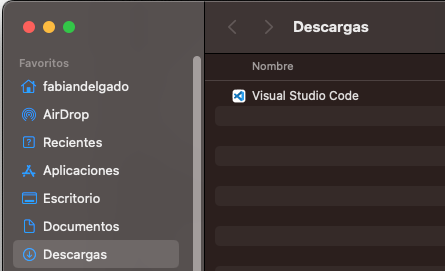
\includegraphics[width=0.7\textwidth]{img/manual/instalar-visual-studio-code.png}
    \caption{Instalar Visual studio code} \label{Img:Instalar+Visual+studio+code}
\end{figure} 

Una vez que lo tenemos instalado en nuestro sistema y abrimos el sofware, hacemos clic en Archivo -> abrir carpeta y ya tendremos nuestro código en el editor.

\subsubsection{Golang}\label{golang}
Golang, también conocido como Go, es un lenguaje de programación de código abierto que se utiliza principalmente para aplicaciones de sistemas, redes y servicios web. Cuenta con compilación estática, lo que significa que el código se compila antes de que se ejecute, y utiliza una recolección de basura eficiente, por lo que los recursos del sistema se emplean de una mejor forma. Asimismo, Golang tiene un modelo de concurrencia incorporado que permite crear aplicaciones que pueden manejar múltiples tareas al mismo tiempo sin afectar el rendimiento. 

Para realizar la instalación, se debe ingresar a la sección de descargas del sitio web oficial de \href{https://go.dev/dl/}{Golang} y seleccionar la versión más reciente (ver figura~\ref{Img:Lista+de+versiones+de+Golang}).

\begin{figure}[h]
    \centering
    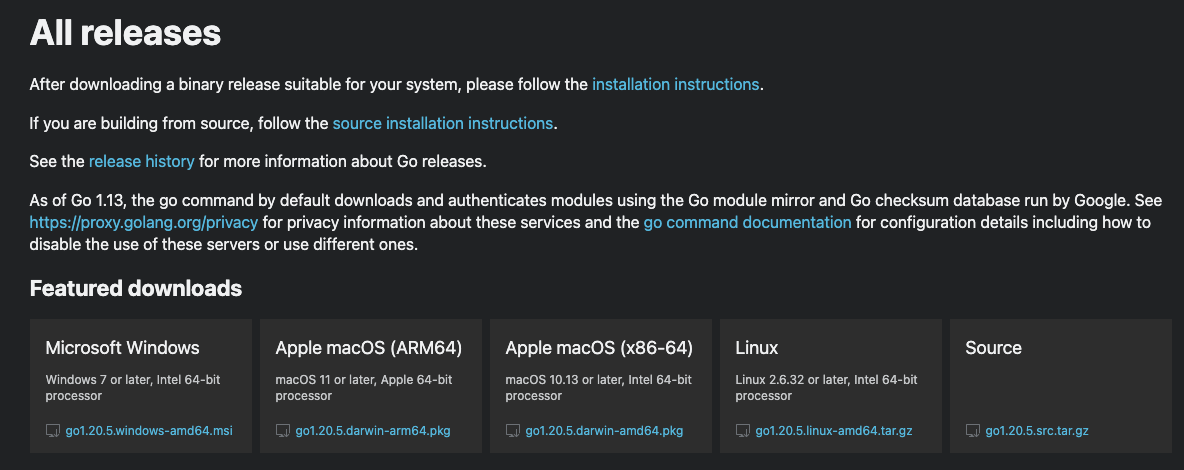
\includegraphics[width=0.7\textwidth]{img/manual/releases.png}
    \caption{Lista de versiones de Golang} \label{Img:Lista+de+versiones+de+Golang}
\end{figure} 

Una vez descargado el paquete de software que instalará Golang en el sistema, basta con iniciarlo y presionar siguiente hasta que se complete la instalación (ver figura~\ref{Img:Instalación+de+Golang}).

\begin{figure}[h]
    \centering
    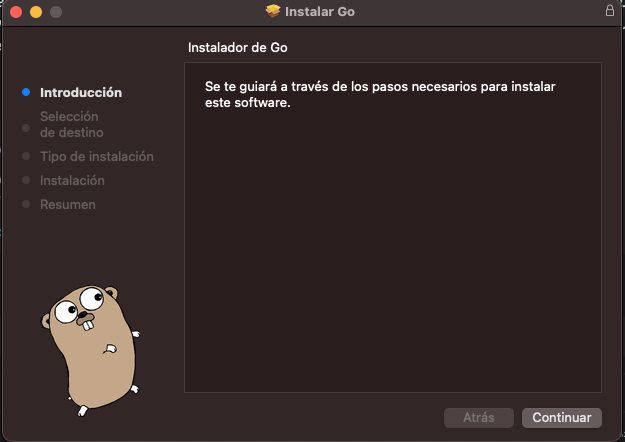
\includegraphics[width=0.7\textwidth]{img/manual/instalacion.png}
    \caption{Instalación de Golang} \label{Img:Instalación+de+Golang}
\end{figure} 

\subsubsection{Python}\label{python}
Python es un lenguaje de programación de alto nivel, orientado a objetos, que presenta una gran cantidad de características similares con otros lenguajes como C++, Java, Modula-3 y Scheme, por lo que ofrece un equilibrio óptimo entre lo práctico y lo conceptual. Es fácil de usar por su sintaxis simple, clara y concisa que facilita su aprendizaje y el mantenimiento de proyectos de gran envergadura, al mismo tiempo, que ofrece un entorno multiplataforma que puede ser ejecutado en diversos sistemas operativos.

Para la instalación de \href{https://www.python.org/downloads/}{Python} hay que ir a su web de descargas, donde la misma detectará nuestra versión de sistema operativo permitiéndonos descargar la última disponible (ver figura~\ref{Img:Lista+de+versiones+de+Python}).

\begin{figure}[h]
    \centering
    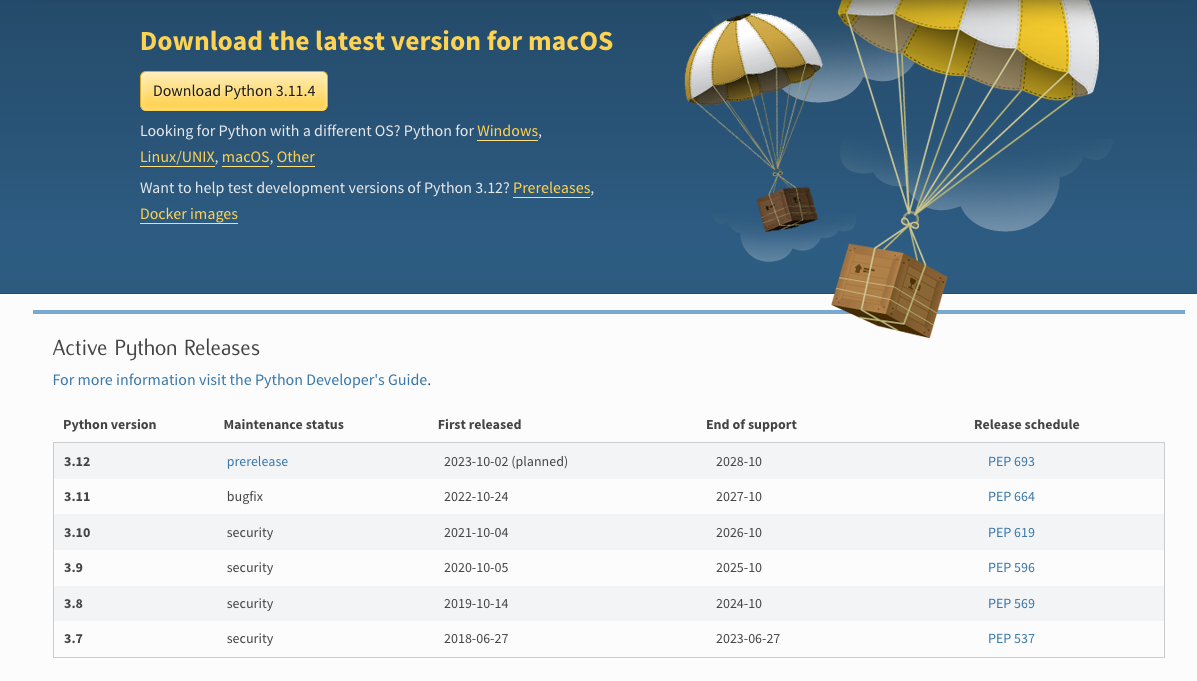
\includegraphics[width=0.5\textwidth]{img/manual/lista-versiones-python.png}
    \caption{Lista de versiones de Python} \label{Img:Lista+de+versiones+de+Python}
\end{figure} 
Una vez que ya contamos con el paquete para instalarlo en nuestro sistema, procedemos a ejecutarlo y damos continuar hasta finalizar la instalación (ver figura~\ref{Img:Instalación+de+Python}).

\begin{figure}[h]
    \centering
    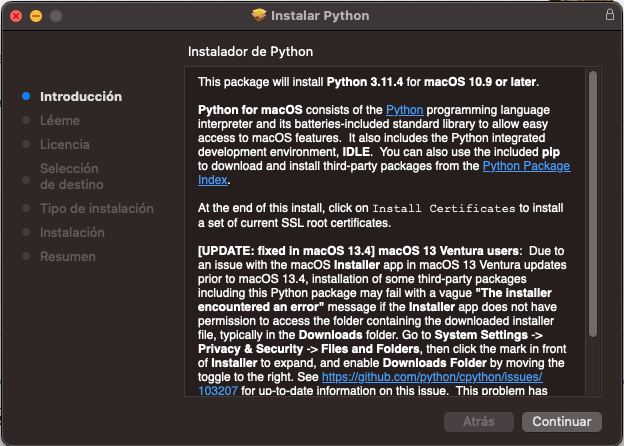
\includegraphics[width=0.7\textwidth]{img/manual/instalacion-python.png}
    \caption{Instalación de Python} \label{Img:Instalación+de+Python}
\end{figure} 

\newpage


\subsubsection{Git}\label{git}
Git es un programa destinado al control de versiones software en el que se registran los cambios producidos en el mismo, facilitando la integración de código por parte de cualquiera de los integrantes del proyecto. En Git cada desarrollador tiene una copia completa del repositorio, pudiendo trabajar de forma independiente sin depender de un servidor central. Por otro lado, Git utiliza un modelo de ramificación y fusión que permite a los desarrolladores trabajar en paralelo en diferentes características o correcciones de errores sin interferir entre sí.

Para poder clonar el repositorio del proyecto y trabajar con él, es necesario contar con Git instalado en el sistema. 
Para instalarlo, podemos navegar a la web de SourceForge y proceder a descargar el instalable de \href{https://sourceforge.net/projects/git-osx-installer/files/git-2.23.0-intel-universal-mavericks.dmg/download?use_mirror=autoselect}{Git} (ver figura~\ref{Img:Instalación+de+Git}).

\begin{figure}[h]
    \centering
    \includegraphics[width=0.7\textwidth]{img/manual/instalar-git.png}
    \caption{Instalación de Git} \label{Img:Instalación+de+Git}
\end{figure} 

\newpage

Luego de este proceso ya podemos clonar el \href{https://github.com/emur-uy}{repositorio} utilizando la url del mismo. Para este fin ejecutamos el siguiente comando git clone -b main git@github.com:emur-uy/backend.git (ver figura~\ref{Img:Clonación+de+repositorio+desde Github}).

\begin{figure}[h]
    \centering
    \includegraphics[width=0.7\textwidth]{img/manual/git-clonado.png}
    \caption{Clonación de repositorio desde Github} \label{Img:Clonación+de+repositorio+desde Github}
\end{figure} 


\subsubsection{Table Plus}\label{table-plus}
TablePlus es un software de gestión de bases de datos con una interfaz gráfica de usuario intuitiva y fácil de usar. Permite a los usuarios conectarse y administrar múltiples bases de datos de manera eficiente y en una sola aplicación, así como navegar por bases de datos relacionales de forma cómoda y sencilla. Ofrece una serie de características útiles como autocompletado de código SQL, la búsqueda de texto completo y la vista de esquema, que hacen que la gestión de bases de datos sea más eficiente y productiva. 

Para instalarlo debemos navegar hasta su \href{https://tableplus.com/}{sitio web}, una vez alli procedemos a hacer click en el botón de descargar (ver figura~\ref{Img:Descarga+de+software+Table+Plus}).

\begin{figure}[h]
    \centering
    \includegraphics[width=0.7\textwidth]{img/manual/table-plus.png}
    \caption{Descarga de software Table Plus.} \label{Img:Descarga+de+software+Table+Plus}
\end{figure} 

Para instalarlo basta con abrir el instalador y arrastra el ícono hacia la carpeta de aplicaciones (ver figura~\ref{Img:Instalación+Table+Plus}).

\begin{figure}[h]
    \centering
    \includegraphics[width=0.7\textwidth]{img/manual/instalacion-table-plus.png}
    \caption{Instalación Table Plus.} \label{Img:Instalación+Table+Plus}
\end{figure} 

Luego ya podemos configurar nuestra instancia de base de datos remota. Para ello, una vez iniciado el software Table Plus completamos con lo datos que se solicitan conforme se aprecia en la siguiente imagen (ver tabla~\ref{tab:requisitos-table-plus}).

\begin{table}[H]
\centering
\begin{tabular}{ll}
\toprule
Campo                     & Valor                           \\
\midrule
\texttt{Name}       & Emur DEV              \\
\texttt{Host}      & db-postgresql-nyc1-56709-do-user-9370728-0.b.db.ondigitalocean.com             \\
\texttt{User}      & emur             \\
\texttt{Password}      &  ver archivo .env      \\
\texttt{Database}      & dev\_emur\_backend           \\
\texttt{Port}      & 25060             \\
\bottomrule
\end{tabular}
\caption{Datos de acceso a la base de datos de desarrollo}
\label{tab:requisitos-table-plus}
\end{table}

A continuación, podemos observar cómo queda configurado en la ventana de Table Plus, listo para conectarse y validando en color verde que fue posible establecer conexión con los datos provistos (ver figura~\ref{Img:Configuración+de+base de+datos+en+Table+Plus}).

\begin{figure}[h]
    \centering
    \includegraphics[width=0.7\textwidth]{img/manual/connect-table-plus.png}
    \caption{Configuración de base de datos en Table Plus.} \label{Img:Configuración+de+base de+datos+en+Table+Plus}
\end{figure} 


\section{Documentación de las APIs}\label{postman}

\subsection{Postman}\label{postman}
Postman es una herramienta de prueba de APIs que permite a los desarrolladores crear, probar, documentar y compartir colecciones de APIs de manera rápida y fácil. En ella, los programadores pueden crear solicitudes HTTP personalizadas y enviarlas a cualquier API en línea o local, y de varias formas, incluyendo GET, POST, PUT, DELETE y PATCH, lo que permite ahorrar tiempo y recursos.

Postman nos permite realizar las pruebas sobre los endpoints de las APIs a medida que queremos corroborar datos o probar nuevos desarrollos sobre las mismas.
Para poder obtener Postman debemos navegar a la zona de \href{https://www.postman.com/downloads/}{descarga} de su sitio web (ver figura~\ref{Img:Descarga+de+Postman})

\begin{figure}[h]
    \centering
    \includegraphics[width=0.9\textwidth]{img/manual/postman-descargas.png}
    \caption{Descarga de Postman.} \label{Img:Descarga+de+Postman}
\end{figure} 

Una vez alli procedemos a descargar la versión que corresponde a nuestro sistema operativo, luego de la descarga procedemos a instalarlo arrastrando el ícono a la carpeta de aplicaciones
(ver figura~\ref{Img:Instalación+de+Postman})

\begin{figure}[h]
    \centering
    \includegraphics[width=0.7\textwidth]{img/manual/postman-instalar.png}
    \caption{Instalación de Postman} \label{Img:Instalación+de+Postman}
\end{figure} 

Seguidamente, se necesita importar la colección que contiene los endpoints de las APIs desarrolladas del backend. Abrimos Postman y nos dirigimos a File -> Import, arrastramos el zip que contiene dichas colecciones y que se encuentra subido al repositorio bajo la carpeta Postman (ver figura~\ref{Img:Abrir+colección+de+Postman})


\begin{figure}[h]
    \centering
    \includegraphics[width=0.7\textwidth]{img/manual/abrir-coleccion-postman.png}
    \caption{Abrir colección de Postman} \label{Img:Abrir+colección+de+Postman}
\end{figure} 

\subsection{Swagger}\label{swagger}
Swagger hace referencia a un conjunto de herramientas, especificaciones y reglas destinadas a la documentación de las APIs. Es fácil de utilizar dada su simplicidad, y la documentación generada puede implementarse directamente en la automatización de procesos dependientes de APIs. Swagger permite hacer pruebas de APIs, y sus elementos, y ofrece compatibilidad con Java, Javascript, Ruby, PHP y Actionscript.

Además del uso de Postman, tal como vimos anteriormente para documentar las APIs, támbien se ha implementado en el proyecto el uso de Swagger permitiendo así contar con una documentación siempre disponible para hacer más fácil el desarrollo de la futura aplicación móvil.

Se puede ingresar a la documentación de Swagger mediante los siguientes links:

\begin{itemize}
\tightlist
\item
  \texttt{Backend}: \href{http://134.209.128.98:8080/docs/index.html}{http://134.209.128.98:8080/docs/index.html}
 \item 
  \texttt{Chatbot}: \href{http://134.209.128.98:5005/apidocs/}{http://134.209.128.98:5005/apidocs/}
\end{itemize}

\begin{figure}[h]
    \centering
    \includegraphics[width=0.7\textwidth]{img/infraestructura/swagger_backend.png}
    \caption{Swagger de Backend} \label{Img:Swagger+backend}
\end{figure} 

\begin{figure}[h]
    \centering
    \includegraphics[width=0.7\textwidth]{img/infraestructura/swagger_chatbot.png}
    \caption{Swagger de Chatbot} \label{Img:Swagger+chatbot}
\end{figure} 

\newpage
\section{Pruebas del sistema}
Para comprobar el correcto funcionamiento del backend, se realizaron tanto pruebas unitarias como funcionales ya que esto permite asegurar la mantenibilidad, correcto funcionamiento ante futuros cambios y corroborar que el sistema continua operando e interoperando con la futura aplicación móvil.

\subsection{Test unitarios}
La finalidad de los test unitarios es asegurar de manera atómica que los módulos desarrollados en el software continúan funcionando ante cambios realizados. Ello permite asegurar que el código actual siga funcionando con la adición del nuevo.

Para realizar las pruebas se utilizó el paquete de Golang llamado testify en conjunto con el framework de Golang GIN, esto permite realizar test y probar el comportamiento de la APIs.
Amerita mencionar que, para las pruebas, se utilizó mocking, ya que permite simular el acceso de información como si de una base de datos se tratara, haciendo posible probar su comportamiento a diferentes situaciones.

En este backend se realizaron 18 test unitarios sobre los servicios asegurando, de esta forma, la lógica de negocio del sistema.

\subsection{Ejecución de los test unitarios}
Para la ejecución de los test unitarios, Golang nos propone el comando "go test -v service/*\_test.go. Dado que éste sólo habilitaba su uso de forma unitaria por cada archivo creado, se procedió a implementar un script que permitiese ejecutar todo el set de pruebas.
Para utilizar dicho script se necesita contar con permisos de ejecución, lo que puede efectuarse a través del comando chmod x ./run\_test.sh.

En las siguientes capturas podemos ver todos los test ejecutándose satisfactoriamente
(ver figura~\ref{Img:Resultado+de+test+parte+1} y ver figura~\ref{Img:Resultado+de+test+parte+2}).

\begin{figure}[h]
    \centering
    \includegraphics[width=0.5\textwidth]{img/manual/test_parte_1.png}
    \caption{Resultado de test parte 1.} \label{Img:Resultado+de+test+parte+1}
\end{figure} 


\begin{figure}[h]
    \centering
    \includegraphics[width=0.5\textwidth]{img/manual/test_parte_2.png}
    \caption{Resultado de test parte 2.} \label{Img:Resultado+de+test+parte+2}
\end{figure} 

\subsection{Test funcionales}

Los test funcionales se encargan de asegurar que los datos de salida del sistema se encuentren operando de acuerdo a lo esperado en la especificaciones.
Asimismo, se centran en realizar las pruebas de interacciones tal como lo haría un usuario del sistema y nos permiten, además, asegurar que el sistema, de cara al usuario, se encuentra funcionando adecuadamente.

En el caso de este proyecto, al tratarse de APIs que serán el backend de la futura aplicación móvil, las pruebas funcionales se realizaron a través de Postman.

La manera de automatizarlas, para evitar probar endpoint por endpoint, ha sido utilizar la funcionalidad Runner de Postman que permite realizar programáticamente la evaluación y asertividad de los datos que espera nuestro frontend.

\begin{figure}[h]
    \centering
    \includegraphics[width=1.0\textwidth]{img/manual/test_admin.png}
    \caption{Resultado de la ejecucíon de los test automatizados de admin.} \label{Img:Resultado+de+test+admin}
\end{figure} 

\begin{figure}[h]
    \centering
    \includegraphics[width=1.1\textwidth]{img/manual/test_usuario.png}
    \caption{Resultado de la ejecucíon de los test automatizados de usuario.} \label{Img:Resultado+de+test+usuario}
\end{figure} 
\newpage
\subsection{Pruebas de estrés}
Estas pruebas se encargan de realizar test de rendimiento sobre el sistema para así determinar su robustez en condiciones de alta concurrencia. Para ello, el sistema se sobrecarga con solicitudes para emular una cantidad de usuarios concurrentes.
De esta forma, se busca identificar los límites del sistema para encontrar cualquier problema que pudiera surgir en cuanto a la performance, ya sea de servidor, código o de acceso a la base de datos para disminuir los tiempos y evitar cuellos de botella.
\begin{figure}[h]
    \centering
    \includegraphics[width=1.0\textwidth]{img/manual/test_de_stress.png}
    \caption{Resultado de la ejecución de los test de stress.} \label{Img:Resultado+de+test+stress}
\end{figure} 




\apendice{Documentación de usuario}

\section{Introducción}
Debido a que el desarrollo se enfocó en la realización del backend, me enfrenté al desafío de identificar cómo podrían hacer los miembros del tribunal evaluador para probar las APIs desarrolladas tanto del backend como del chatbot, no existiendo aún la aplicación como tal.
Para ello me desafié a buscar una solución que permitiera ejecutarse en la nube de forma que no fuera necesario instalar un software en cada computadora para las pruebas.

\section{Requisitos de usuarios}
Como herramienta de pruebas para los usuarios se ha seleccionado Postman Web ya que sólo con contar con un navegador web es suficiente para este software.

A continuación, se detallan los requisitos mínimos para poder ejecutarse las pruebas, en base al navegador del que se disponga.

\begin{itemize}
\tightlist
\item
  \texttt{Chrome}: versión 78 o superior.
  \item
  \texttt{Firefox}: versión 76 o superior.
  \item
  \texttt{Edge}: versión 79 o superior.
  \item
  \texttt{Safari}: versión 13.1.1 o superior.
\end{itemize}

\section{Manual del usuario}

\subsection{Backend}

Para poder realizar las pruebas los usuarios deberán de navegar a la siguiente url: \href{https://www.postman.com/cloudy-space-109868/workspace/emur/collection/27053529-4afae92f-7a66-4091-ad9b-50f499e2d515}{Postman Web}.\\
Allí encontrarán las colecciones de endpoints creadas para el backend y chatbot de la futura aplicación móvil de EM (ver figura~\ref{Img:Coleccion+Postman+Usuario}).
\begin{figure}[h]
    \centering
    \includegraphics[width=1.1\textwidth]{img/usuario/colecciones_postman1.png}
    \caption{Colección de APIs de Backend y Chatbot} \label{Img:Coleccion+Postman+Usuario}
\end{figure} 

Una vez allí, las colecciones se muestran colapsadas, para tal fin debemos hacer clic sobre la colección que queremos abrir. En el caso del presente proyecto, existen 3 colecciones debido a que una es para probar con rol administrador, otra es con el rol de usuario y la tercera para probar el chatbot (ver figura~\ref{Img:Coleccion+Postman+Usuario+2}).

\newpage
\begin{figure}[h]
    \centering
    \includegraphics[width=0.8\textwidth]{img/usuario/colecciones_postman2.png}
    \caption{Cómo abrir las colecciones} \label{Img:Coleccion+Postman+Usuario+2}
\end{figure} 

Una vez tenemos la colección abierta podemos proceder a probar los endpoints. A continuación se explica cómo hacerlo.

\begin{itemize}
\tightlist
\item
  \texttt{Paso 1}: Clic en el menú izquierdo sobre [QUESTION] - CREATE
  \item
  \texttt{Paso 2}: Nos dirigimos a Body.
  \item
  \texttt{Paso 3}: En el apartado 3, remplazamos el contenido a la key llamada text con el texto que se desee.
  \item
  \texttt{Paso  4}: Presionamos sobre Send.
    \item
  \texttt{Paso  5}: Observamos el resultado del operación ejecutada.
\end{itemize}

Con los puntos anteriores podemos fácilmente manejar la creación de request hacía la API para acceder a las diferentes operaciones que tendrá la futura aplicación móvil.
A modo de mejor entendimiento, se disponibiliza un video en el siguiente enlace:
\href{https://www.dropbox.com/s/3b3uwcgpcwrhlkx/grabacion_question_answer.mov?dl=0}{Video en Dropbox}

A modo de facilitar las pruebas, los endpoints en Postman cuentan con datos precargados.

\subsection{Chatbot}

Para el caso del chatbot, las pruebas se realizan de la misma forma, se ha disponibilizado bajo una colección llamada Chatbot, donde se puede acceder al endpoint para realizar las preguntas que se deseen.

También, a modo de tutorial, se ha disponibilizado un video en el siguiente enlace:
\href{https://www.dropbox.com/s/hgilnzncrb17aju/chatbot.mov?dl=0}{Video en Dropbox}








\bibliographystyle{plain}
\bibliography{bibliografiaAnexos}

\end{document}
